% Options for packages loaded elsewhere
\PassOptionsToPackage{unicode}{hyperref}
\PassOptionsToPackage{hyphens}{url}
%
\documentclass[
]{book}
\usepackage{amsmath,amssymb}
\usepackage{iftex}
\ifPDFTeX
  \usepackage[T1]{fontenc}
  \usepackage[utf8]{inputenc}
  \usepackage{textcomp} % provide euro and other symbols
\else % if luatex or xetex
  \usepackage{unicode-math} % this also loads fontspec
  \defaultfontfeatures{Scale=MatchLowercase}
  \defaultfontfeatures[\rmfamily]{Ligatures=TeX,Scale=1}
\fi
\usepackage{lmodern}
\ifPDFTeX\else
  % xetex/luatex font selection
\fi
% Use upquote if available, for straight quotes in verbatim environments
\IfFileExists{upquote.sty}{\usepackage{upquote}}{}
\IfFileExists{microtype.sty}{% use microtype if available
  \usepackage[]{microtype}
  \UseMicrotypeSet[protrusion]{basicmath} % disable protrusion for tt fonts
}{}
\makeatletter
\@ifundefined{KOMAClassName}{% if non-KOMA class
  \IfFileExists{parskip.sty}{%
    \usepackage{parskip}
  }{% else
    \setlength{\parindent}{0pt}
    \setlength{\parskip}{6pt plus 2pt minus 1pt}}
}{% if KOMA class
  \KOMAoptions{parskip=half}}
\makeatother
\usepackage{xcolor}
\usepackage{color}
\usepackage{fancyvrb}
\newcommand{\VerbBar}{|}
\newcommand{\VERB}{\Verb[commandchars=\\\{\}]}
\DefineVerbatimEnvironment{Highlighting}{Verbatim}{commandchars=\\\{\}}
% Add ',fontsize=\small' for more characters per line
\usepackage{framed}
\definecolor{shadecolor}{RGB}{248,248,248}
\newenvironment{Shaded}{\begin{snugshade}}{\end{snugshade}}
\newcommand{\AlertTok}[1]{\textcolor[rgb]{0.94,0.16,0.16}{#1}}
\newcommand{\AnnotationTok}[1]{\textcolor[rgb]{0.56,0.35,0.01}{\textbf{\textit{#1}}}}
\newcommand{\AttributeTok}[1]{\textcolor[rgb]{0.13,0.29,0.53}{#1}}
\newcommand{\BaseNTok}[1]{\textcolor[rgb]{0.00,0.00,0.81}{#1}}
\newcommand{\BuiltInTok}[1]{#1}
\newcommand{\CharTok}[1]{\textcolor[rgb]{0.31,0.60,0.02}{#1}}
\newcommand{\CommentTok}[1]{\textcolor[rgb]{0.56,0.35,0.01}{\textit{#1}}}
\newcommand{\CommentVarTok}[1]{\textcolor[rgb]{0.56,0.35,0.01}{\textbf{\textit{#1}}}}
\newcommand{\ConstantTok}[1]{\textcolor[rgb]{0.56,0.35,0.01}{#1}}
\newcommand{\ControlFlowTok}[1]{\textcolor[rgb]{0.13,0.29,0.53}{\textbf{#1}}}
\newcommand{\DataTypeTok}[1]{\textcolor[rgb]{0.13,0.29,0.53}{#1}}
\newcommand{\DecValTok}[1]{\textcolor[rgb]{0.00,0.00,0.81}{#1}}
\newcommand{\DocumentationTok}[1]{\textcolor[rgb]{0.56,0.35,0.01}{\textbf{\textit{#1}}}}
\newcommand{\ErrorTok}[1]{\textcolor[rgb]{0.64,0.00,0.00}{\textbf{#1}}}
\newcommand{\ExtensionTok}[1]{#1}
\newcommand{\FloatTok}[1]{\textcolor[rgb]{0.00,0.00,0.81}{#1}}
\newcommand{\FunctionTok}[1]{\textcolor[rgb]{0.13,0.29,0.53}{\textbf{#1}}}
\newcommand{\ImportTok}[1]{#1}
\newcommand{\InformationTok}[1]{\textcolor[rgb]{0.56,0.35,0.01}{\textbf{\textit{#1}}}}
\newcommand{\KeywordTok}[1]{\textcolor[rgb]{0.13,0.29,0.53}{\textbf{#1}}}
\newcommand{\NormalTok}[1]{#1}
\newcommand{\OperatorTok}[1]{\textcolor[rgb]{0.81,0.36,0.00}{\textbf{#1}}}
\newcommand{\OtherTok}[1]{\textcolor[rgb]{0.56,0.35,0.01}{#1}}
\newcommand{\PreprocessorTok}[1]{\textcolor[rgb]{0.56,0.35,0.01}{\textit{#1}}}
\newcommand{\RegionMarkerTok}[1]{#1}
\newcommand{\SpecialCharTok}[1]{\textcolor[rgb]{0.81,0.36,0.00}{\textbf{#1}}}
\newcommand{\SpecialStringTok}[1]{\textcolor[rgb]{0.31,0.60,0.02}{#1}}
\newcommand{\StringTok}[1]{\textcolor[rgb]{0.31,0.60,0.02}{#1}}
\newcommand{\VariableTok}[1]{\textcolor[rgb]{0.00,0.00,0.00}{#1}}
\newcommand{\VerbatimStringTok}[1]{\textcolor[rgb]{0.31,0.60,0.02}{#1}}
\newcommand{\WarningTok}[1]{\textcolor[rgb]{0.56,0.35,0.01}{\textbf{\textit{#1}}}}
\usepackage{longtable,booktabs,array}
\usepackage{calc} % for calculating minipage widths
% Correct order of tables after \paragraph or \subparagraph
\usepackage{etoolbox}
\makeatletter
\patchcmd\longtable{\par}{\if@noskipsec\mbox{}\fi\par}{}{}
\makeatother
% Allow footnotes in longtable head/foot
\IfFileExists{footnotehyper.sty}{\usepackage{footnotehyper}}{\usepackage{footnote}}
\makesavenoteenv{longtable}
\usepackage{graphicx}
\makeatletter
\def\maxwidth{\ifdim\Gin@nat@width>\linewidth\linewidth\else\Gin@nat@width\fi}
\def\maxheight{\ifdim\Gin@nat@height>\textheight\textheight\else\Gin@nat@height\fi}
\makeatother
% Scale images if necessary, so that they will not overflow the page
% margins by default, and it is still possible to overwrite the defaults
% using explicit options in \includegraphics[width, height, ...]{}
\setkeys{Gin}{width=\maxwidth,height=\maxheight,keepaspectratio}
% Set default figure placement to htbp
\makeatletter
\def\fps@figure{htbp}
\makeatother
\setlength{\emergencystretch}{3em} % prevent overfull lines
\providecommand{\tightlist}{%
  \setlength{\itemsep}{0pt}\setlength{\parskip}{0pt}}
\setcounter{secnumdepth}{5}
\usepackage{booktabs}
\ifLuaTeX
  \usepackage{selnolig}  % disable illegal ligatures
\fi
\usepackage[]{natbib}
\bibliographystyle{apalike}
\IfFileExists{bookmark.sty}{\usepackage{bookmark}}{\usepackage{hyperref}}
\IfFileExists{xurl.sty}{\usepackage{xurl}}{} % add URL line breaks if available
\urlstyle{same}
\hypersetup{
  pdftitle={Incorporating Spatial Analysis into Agricultural Field Experiments.},
  pdfauthor={Julia Piaskowski; William Price},
  hidelinks,
  pdfcreator={LaTeX via pandoc}}

\title{Incorporating Spatial Analysis into Agricultural Field Experiments.}
\author{Julia Piaskowski\footnote{University of Idaho, \href{mailto:jpiaskowski@uidaho.edu}{\nolinkurl{jpiaskowski@uidaho.edu}}} \and William Price\footnote{University of Idaho, \href{mailto:bprice@uidaho.edu}{\nolinkurl{bprice@uidaho.edu}}}}
\date{August 21, 2023}

\begin{document}
\maketitle

{
\setcounter{tocdepth}{1}
\tableofcontents
}
\hypertarget{preface}{%
\chapter{Preface}\label{preface}}

\begin{center}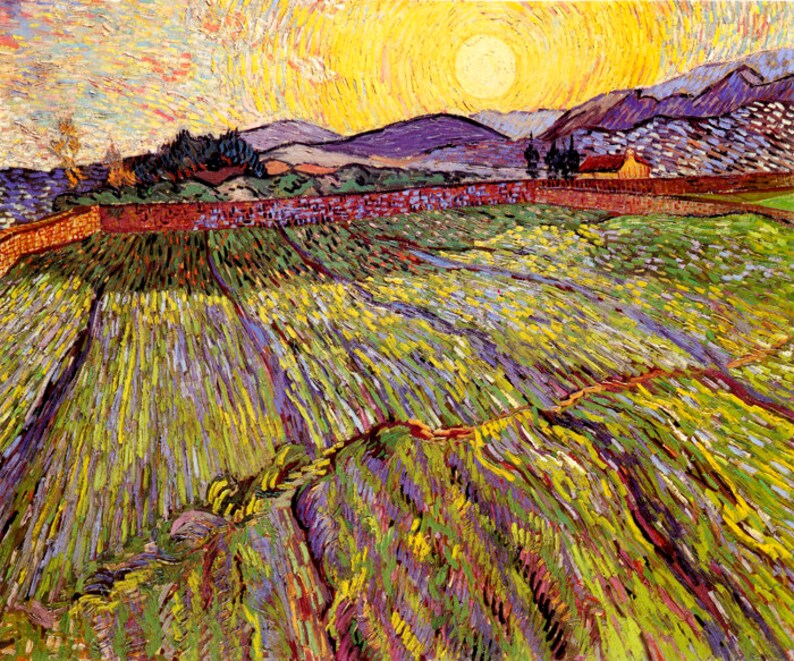
\includegraphics[width=0.9\linewidth]{img/wheat_field_van_gogh} \end{center}

Vincent Van Gogh

\hypertarget{tutorial-goal}{%
\section{Tutorial goal}\label{tutorial-goal}}

\emph{To help people conducting planned agricultural field trials understand and incorporate spatial variation routinely into analysis of field trials.}

Current educational resources are focused largely on geospatial applications that typically require a a moderate to deep understanding of mapping tools and spatial analytic techniques. Furthermore, there is not a comprehensive resources for spatial analytic techniques for field experiments that is also freely available. This tutorial is intended to fill that gap.

\hypertarget{prerequisites}{%
\section{Prerequisites}\label{prerequisites}}

In order to run the scripts in this demonstration, you will to download R, available free through the \href{https://cran.r-project.org/}{Comprehensive R Archive Network} (CRAN). While this is sufficient for running R scripts, You may also find it helpful to use RStudio, which provides a nice graphical user interface for R. RStudio can be downloaded \href{https://www.rstudio.com/products/rstudio/download/}{here}.

If you already have R installed, please make sure you have version 4.0.0 or newer.

This demonstration is not intended to provide instructions on general R usage. However, There are numerous web resources for learning the Basics of R. \href{https://software-carpentry.org/lessons/}{Software carpentry} offers several lesson plans covering the foundation of R.

\hypertarget{r-requirements}{%
\section{R requirements}\label{r-requirements}}

This tutorial was built using R version 4.1 (``Camp Pontanezen''). R session information is provided in section \ref{the-end}.

\textbf{R Packages used in this tutorial}

\begin{longtable}[]{@{}ll@{}}
\toprule\noalign{}
Package & Usage in This Tutorial \\
\midrule\noalign{}
\endhead
\bottomrule\noalign{}
\endlastfoot
dplyr, tidyr, purrr & basic data manipulation \\
ggplot, desplot & plotting \\
agridat & contains demonstration data sets \\
sp, sf & standard manipulation of spatial objects \\
spdep & spatial dependence functions \\
gstat & empirical variogram estimation \\
nlme, lme4 & mixed model analysis \\
emmeans & extract treatments means \\
spaMM & Matérn covariance structure \\
SpATS & spatial splines for field trials \\
breedR & mixed modelling with AR1xAR1 estimation \\
\end{longtable}

All packages aside from \textbf{breedR} are available on CRAN. The package \textbf{breedR}, is available on GitHub can be installed within R with the following code:

\begin{verbatim}
remotes::install_github("famuvie/breedR")
\end{verbatim}

\hypertarget{sas-requirements}{%
\section{SAS requirements}\label{sas-requirements}}

In order to run the SAS portion of this tutorial, a valid copy of SAS Base and Stat products and a current SAS license are required. This tutorial was built using SAS 9.4 (TS1M5). Although older versions of SAS may also work, we have not evaluated this. Users can also consider downloading and using a free version of \href{https://www.sas.com/en_us/software/on-demand-for-academics/references/getting-started-with-sas-ondemand-for-academics-studio.html}{SAS® On Demand for Academics: Studio}.

\textbf{SAS procedures used in this tutorial}

\begin{longtable}[]{@{}ll@{}}
\toprule\noalign{}
Procedure & Usage in This Tutorial \\
\midrule\noalign{}
\endhead
\bottomrule\noalign{}
\endlastfoot
FORMAT, DATA, PRINT & basic data input, manipulation, and display \\
SORT, RANK & sort and rank estimated means \\
SGPLOT & plotting \\
MIXED, GLIMMIX & mixed model analysis \\
VARIOGRAM & empirical variogram estimation \\
\end{longtable}

\hypertarget{contributors}{%
\section{Contributors}\label{contributors}}

\href{mailto:jpiaskowski@uidaho.edu}{Julia Piaskowski} wrote the R sections and William Price wrote the SAS portions of this tutorial.

This book was written in \href{https://bookdown.org/yihui/bookdown}{bookdown}.

\hypertarget{license}{%
\section{License}\label{license}}

Incorporating Spatial Analysis into Agricultural Field Experiments by Julia Piaskowski and William Price is licensed under a \href{https://creativecommons.org/licenses/by-nc/4.0/}{Creative Commons Attribution-NonCommercial 4.0 International License}

\begin{center}
\includegraphics[width=0.2\linewidth]{img/CC-by-nc} \end{center}

\hypertarget{intro}{%
\chapter{Introduction}\label{intro}}

\hypertarget{why-care-about-spatial-variation}{%
\section{Why care about spatial variation?}\label{why-care-about-spatial-variation}}

The goal of many agricultural field trials is to provide information about crop response to a set a treatments such as soil treatments, disease pressure or crop genetic variation. Agricultural field trials employ common experimental designs such as randomized complete block design to account for environmental heterogeneity. However, those techniques are quite often inadequate to fully account for spatial heterogeneity that arises due to field position, soil conditions, disease, wildlife impacts and more.

\begin{center}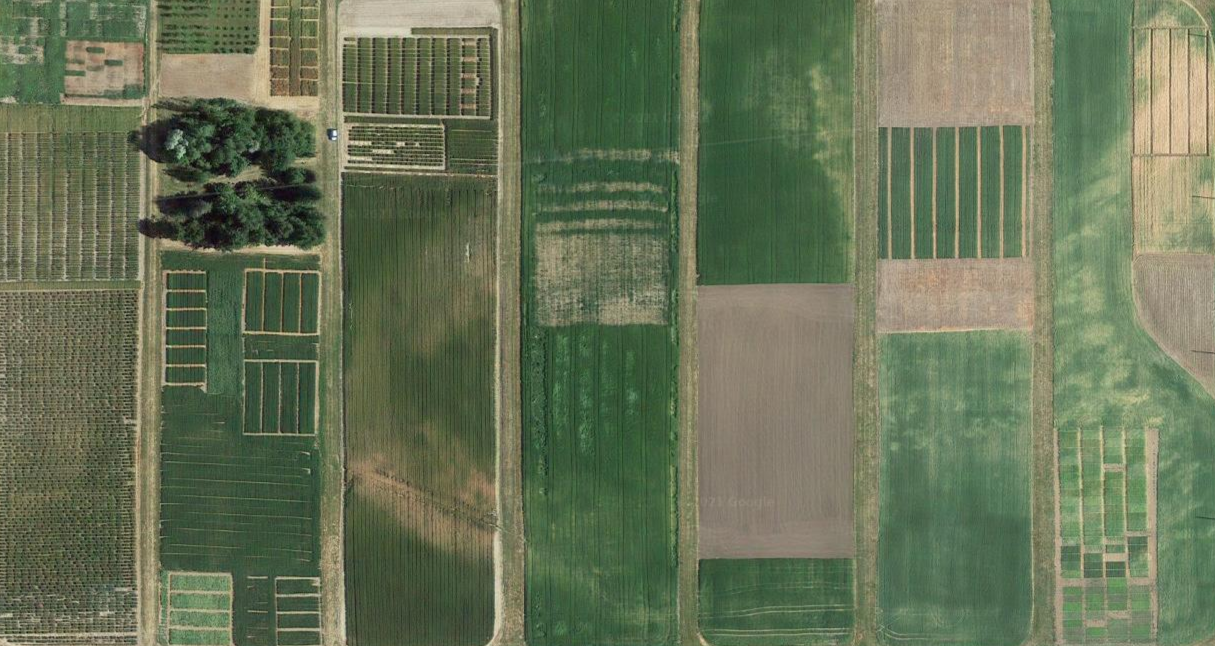
\includegraphics[width=0.9\linewidth]{img/plant_sciences_farm} \end{center}

\emph{University Research Farm}

When spatial autocorrelation is not accounted for in an analysis, the result can be incorrect treatment estimates, correlated errors (that violate the assumption of linear models and invalidate the analysis) and low experimental power. Incorporating spatial correlation between experimental plots can improve the overall accuracy and precision of these estimates.

\hypertarget{diagnosing-spatial-auto-correlation}{%
\section{Diagnosing spatial auto-correlation}\label{diagnosing-spatial-auto-correlation}}

Spatial correlation is similarity of plots that are close to one another. That correlation is expected to decline with distance. This is different from experiment-wide gradients, such as a salinity gradient or position on a slope.

\hypertarget{morans-i}{%
\subsection{Moran's I}\label{morans-i}}

Moran's I, sometimes called ``Global Moran's I'' is similar to a correlation coefficient. It is a test for correlation between units (plots in our case).

\[ I = \frac{N}{W}\frac{\sum_i \sum_j w_{ij} (x_i - \bar{x})(x_j - \bar{x})}{\sum_i(x_i - \bar{x})^2} 
\qquad i \neq j\]
and \(j\), x is the variable of interest, \(w_{ij}\) are a spatial weights between each \(i\) and \(j\), and W is the sum of all weights. The expected values of Moran's I is \(-1/(N-1)\). Values greater than that indicate positive spatial correlation (areas close to each other are similar), while values less than the expected Moran's I indicate dissimilarity as spatial distance between points decreases.
Where N is total number of spatial locations indexed by \(i\)

There are several options for defining adjacent neighbors and how to weight each neighbor's influence. The two common configurations for defining neighbors are the rook and queen configurations. These are exactly what their chess analogy suggests: ``rook'' defines neighbors in an row/column fashion, while ``queen'' defines neighbors in a row/column configuration an also neighbors located diagonally at a 45 degree angle from the row/column neighbors. Determining this can be somewhat complicated when working with irregularly-placed data (e.g.~county seats), but is quite unambiguous for lattice data common in planned field experiments:

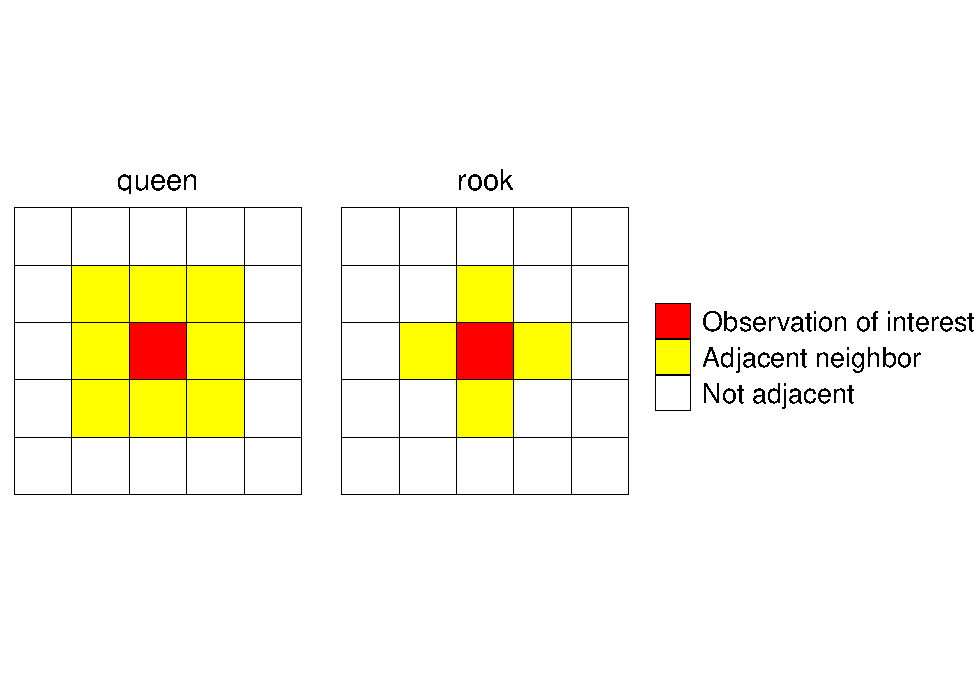
\includegraphics{Field-Trial-Spatial-Analysis-Guide_files/figure-latex/unnamed-chunk-5-1.pdf}

Another test for diagnosing spatial correlation is Geary's C:

\[ I = \frac{(N -1)}{2W}\frac{\sum_i \sum_j w_{ij} (x_i - x_j)^2}{\sum_i(x_i - \bar{x})^2} \qquad i \neq j\]

These terms have the same meaning in Moran's I. The expected value of Geary's C is 1. Values higher than 1 indicate positive spatial correlation and less than 1 indicate negative spatial correlation.

\hypertarget{empirical-variogram-semivariance}{%
\subsection{Empirical variogram \& semivariance}\label{empirical-variogram-semivariance}}

An empirical variogram is a visual tool for understanding how error terms are related to each other over spatial distance. It relies on semivariance (\(\gamma\)), a statistic expressing variance as a function of pairwise distances between data points at points \(i\) and \(j\).

\[\gamma(h) = \frac{1}{2|N(h)|}\sum_{N(h)}(x_i - x_j)^2\]

Semivariances are binned for distance intervals. The average values for semivariance and distance interval can be fit to correlated error models such a exponential, spherical, Gaussian and Matérn. How to do this is explored further in \ref{background} of this guide.

Three important concepts of an empirical variogram are \emph{nugget}, \emph{sill} and \emph{range}

\begin{figure}
\centering
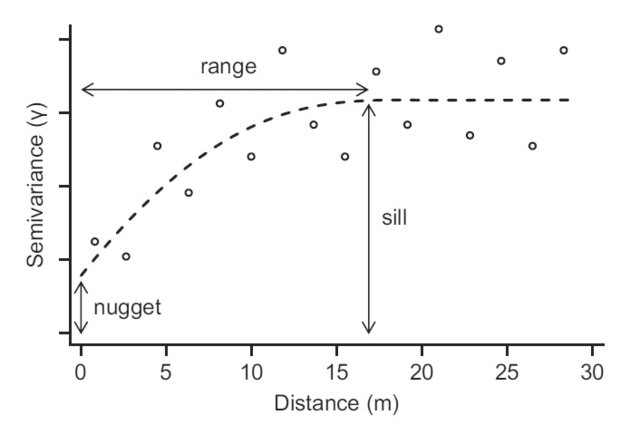
\includegraphics{img/Sadoti2014_spherical.jpg}
\caption{Example Empirical Variogram}
\end{figure}

\begin{itemize}
\tightlist
\item
  range = distance up to which is there is spatial correlation
\item
  sill = uncorrelated variance of the variable of interest
\item
  nugget = measurement error, or short-distance spatial variance and other unaccounted for variance
\end{itemize}

\textbf{2 other concepts:}

\begin{itemize}
\tightlist
\item
  partial sill = sill - nugget
\item
  nugget effect = the nugget/sill ratio, interpreted opposite of \(r^2\)
\end{itemize}

\hypertarget{background}{%
\chapter{Spatial Models}\label{background}}

This section contains some of the statistical background behind why spatial models are used and how they work. Understanding this section is not essential, but it is extremely helpful. This section relies on information introduced in \ref{intro}, so please make sure you have read that section if you are new to empirical variograms and spatial statistics.

General linear statistical models are commonly modeled as thus:

\[Y_i = \beta_0 + X_i\beta_1 + \epsilon_i\]
\(\beta_1\) is a slope describing the relationship between a continuous variable and the dependent variable, \(Y_i\). If \(X_i\) is a categorical variable, such as a crop variety, then there will be \(p-1\) slopes estimated, where p is the number of unique treatments levels in \(X\).

The error terms, \(\epsilon_i\) are assumed normally distributed with a mean of zero and a variance of \(\sigma^2\) :

\[e_i ~\sim N(0, \sigma^2)\]
The error terms, or residuals, are assumed to be \emph{identically} and \emph{independently} distributed (sometimes abbreviated ``iid''). This implies a constant variance of the error terms and zero covariance between residuals.

If N = 3, the expanded model looks like this:

\[\left[ {\begin{array}{ccc} Y_1\\ Y_2\\ Y_3 \end{array} } \right] = \beta_0 + 
\left[ {\begin{array}{ccc} X_1\\ X_2\\ X_3 \end{array}  } \right] \beta_1 +
\left[ {\begin{array}{ccc} \epsilon_1\\ \epsilon_2\\ \epsilon_3 \end{array}  } \right] \]

\[e_i ~\sim N \Bigg( 0, 
\left[ {\begin{array}{ccc} \sigma^2 & 0 & 0 \\ 0 & \sigma^2 & 0\\ 0 & 0 & \sigma^2\end{array}  } \right] \Bigg) \]

If spatial variation is present, the off-diagonals of the variance-covariance matrix are not zero - hence the error terms are not independently distributed. As a result, hypotheses test and parameter estimates from uncorrected linear models will provide erroneous results.

\hypertarget{correlated-error-models}{%
\section{Correlated error models}\label{correlated-error-models}}

\hypertarget{distance-based-correlation-error-models}{%
\subsection{Distance-based correlation error models}\label{distance-based-correlation-error-models}}

There are mathematical tools for modelling how error terms are correlated with each other based on pairwise physical distance between observations. These models can be used to weight observations. Often, the data are assumed to be \emph{isotropic}, where distance but not direction impacts the spatial error correlation.

There are several methods for estimating the semivariance as a direct function of distance.

\hypertarget{exponential}{%
\subsubsection{Exponential}\label{exponential}}

\[ \gamma (h)\left\{ {\begin{array}{cc} 0 & h = 0\\ C_0+C_1 \left [ 1-e^{-(\frac{h}{r})} \right] & h > 0 \end{array} } \right. \]
where

\[ C_0 = nugget \\ C_1 = partial \: sill \\ r = range\]

\begin{figure}

{\centering 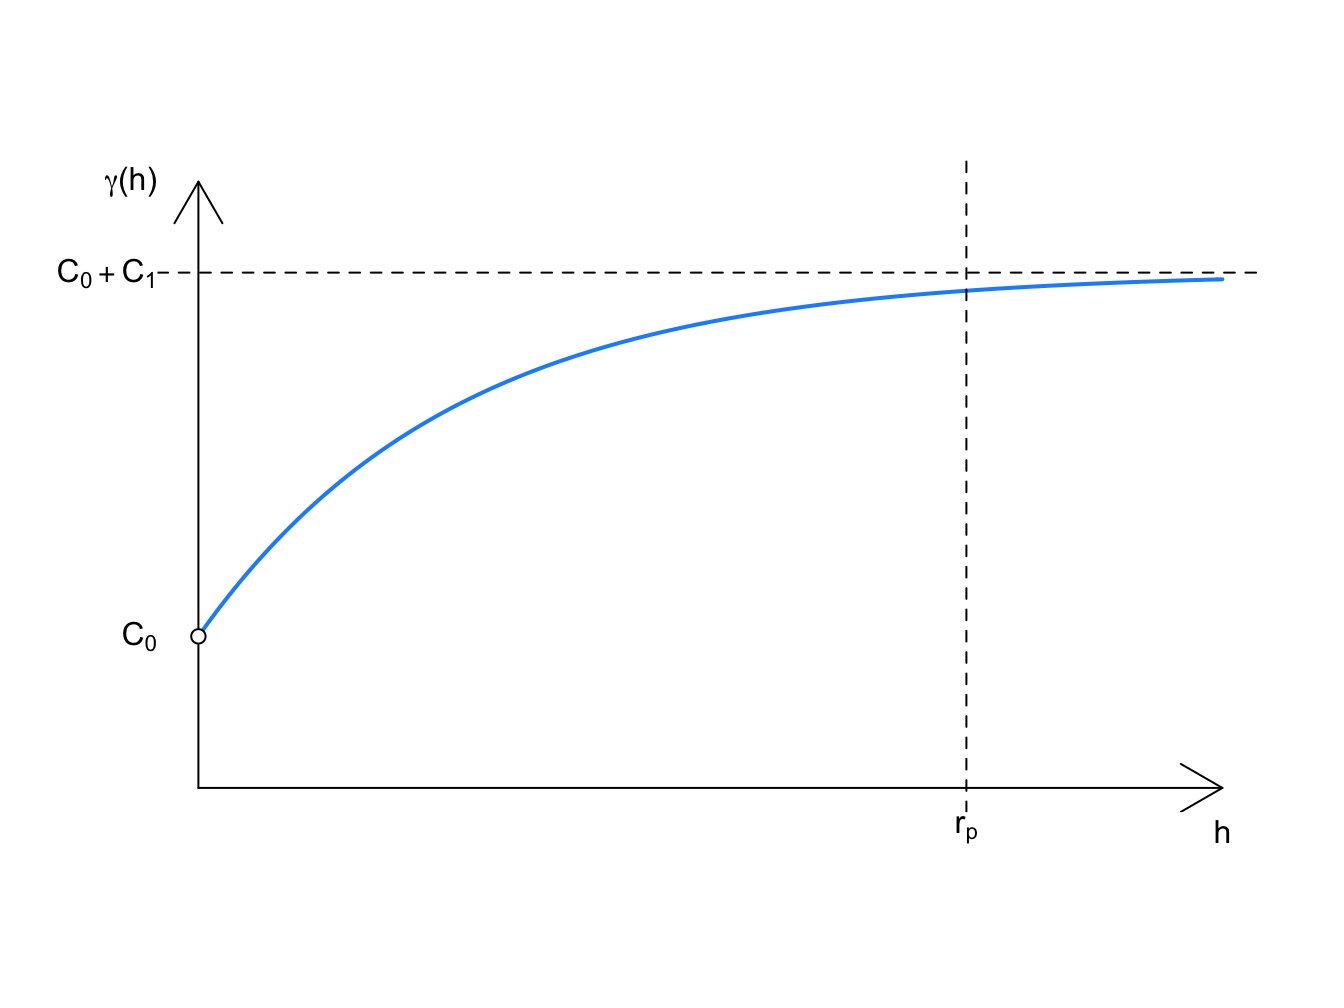
\includegraphics[width=0.7\linewidth]{Field-Trial-Spatial-Analysis-Guide_files/figure-latex/Exp-CE-fig-1} 

}

\caption{Exponential Model}\label{fig:Exp-CE-fig}
\end{figure}

\(3r = r_p\) is the ``practical range'', which is 95\% of the true value for \(C_1\).

\hypertarget{gaussian}{%
\subsubsection{Gaussian}\label{gaussian}}

(a squared version of the exponential model)

\[ \gamma (h)\left\{ {\begin{array}{cc} 0 & h = 0\\ C_0+C_1 \left [ 1-e^{-(\frac{h}{r})^2} \right] & h > 0 \end{array} } \right. \]
where

\[ C_0 = nugget \\ C_1 = partial \: sill \\ r = range\]

\begin{figure}

{\centering 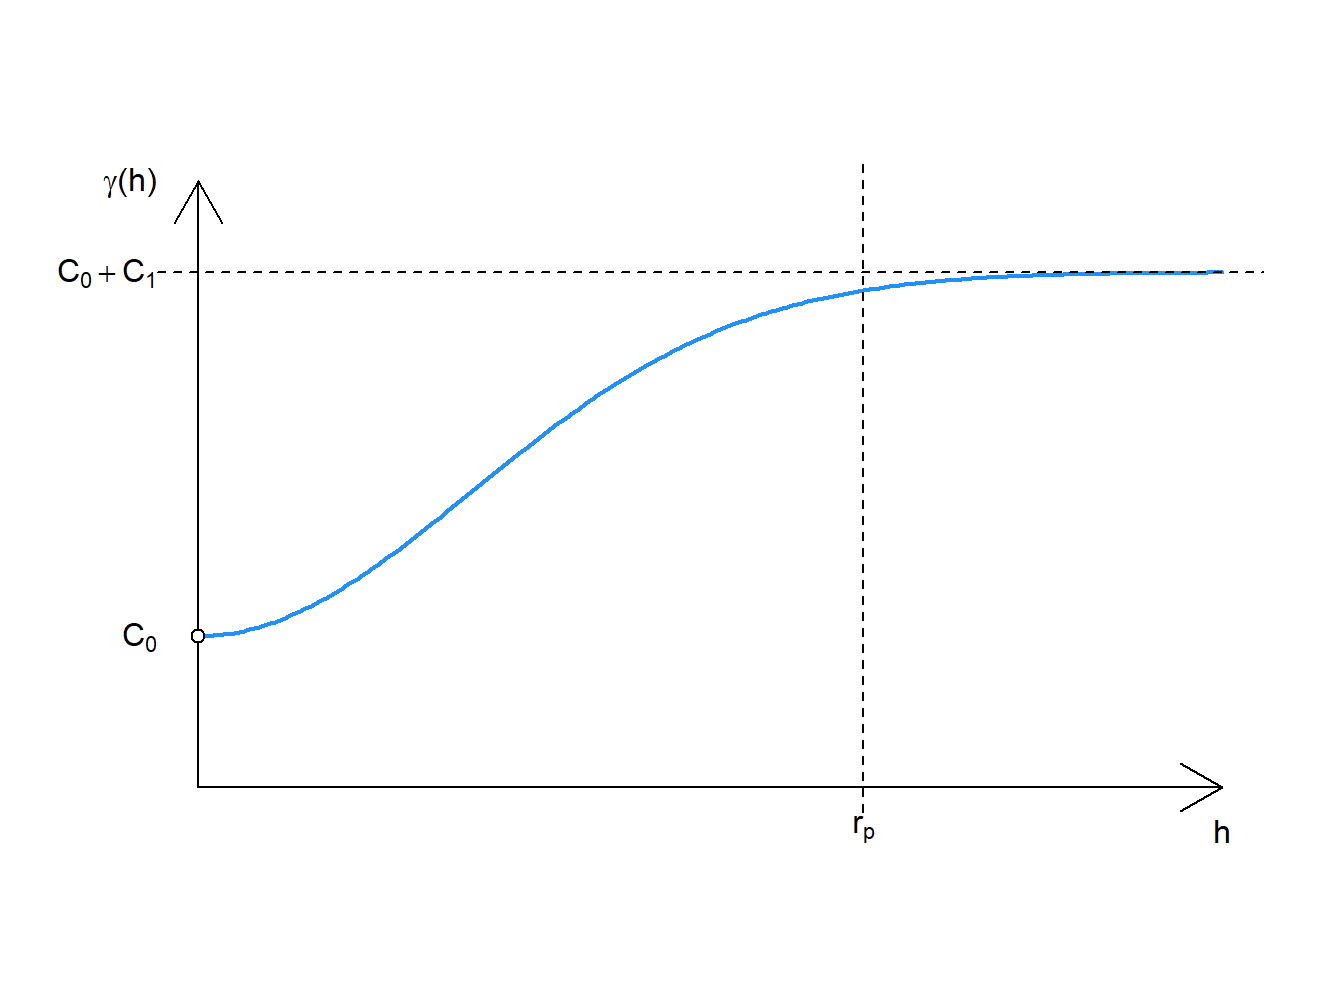
\includegraphics[width=0.7\linewidth]{Field-Trial-Spatial-Analysis-Guide_files/figure-latex/Gau-CE-fig-1} 

}

\caption{Gaussian Model}\label{fig:Gau-CE-fig}
\end{figure}

\(\sqrt 3r = r_p\) is the ``practical range'', which is 95\% of the true value for \(C_1\).

\hypertarget{spherical}{%
\subsubsection{Spherical}\label{spherical}}

\[ \gamma (h) = \left\{ {\begin{array}{cc} 0 & h = 0\\ C_0+C_1 \left[ \frac{3h}{2r}-0.5\bigg( \frac{h}{r}\bigg)^3 \right] & 0 <h \leq r \\ 
C_0 + C_1 & h > r \end{array} } \right. \]
where

\[ C_0 = nugget \\ C_1 = partial \: sill \\ r = range\]

\begin{figure}

{\centering 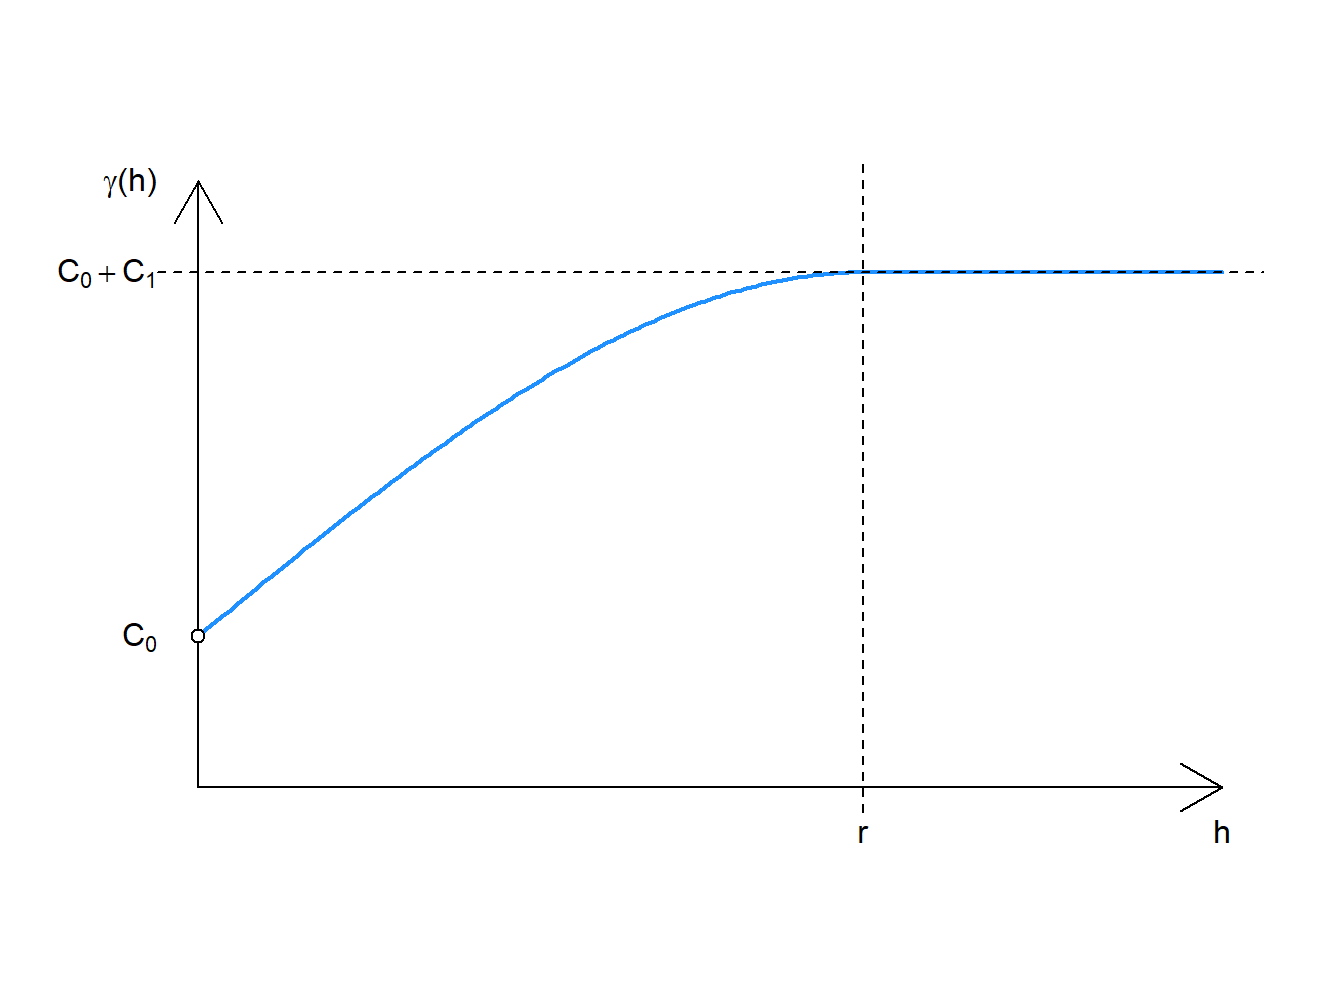
\includegraphics[width=0.7\linewidth]{Field-Trial-Spatial-Analysis-Guide_files/figure-latex/Sph-CE-fig-1} 

}

\caption{Spherical Model}\label{fig:Sph-CE-fig}
\end{figure}

\hypertarget{other-correlated-error-distance-models}{%
\subsubsection{Other correlated error distance models}\label{other-correlated-error-distance-models}}

There are many more models - Matérn, Cauchy, Logistic - that may describe spatial correlation in a data set.

There are two addition models that have no range or sill, the linear model and power model. If your data fits these, consider doing a trend analysis.

\hypertarget{linear}{%
\subsubsection{Linear}\label{linear}}

\[ \gamma (h)=\left\{ {\begin{array}{cc} 0 & h = 0\\ C_0+C_1h & h > 0 \end{array} } \right. \]
where

\[ C_0 = nugget \\ C_1 = slope \]

\begin{figure}

{\centering 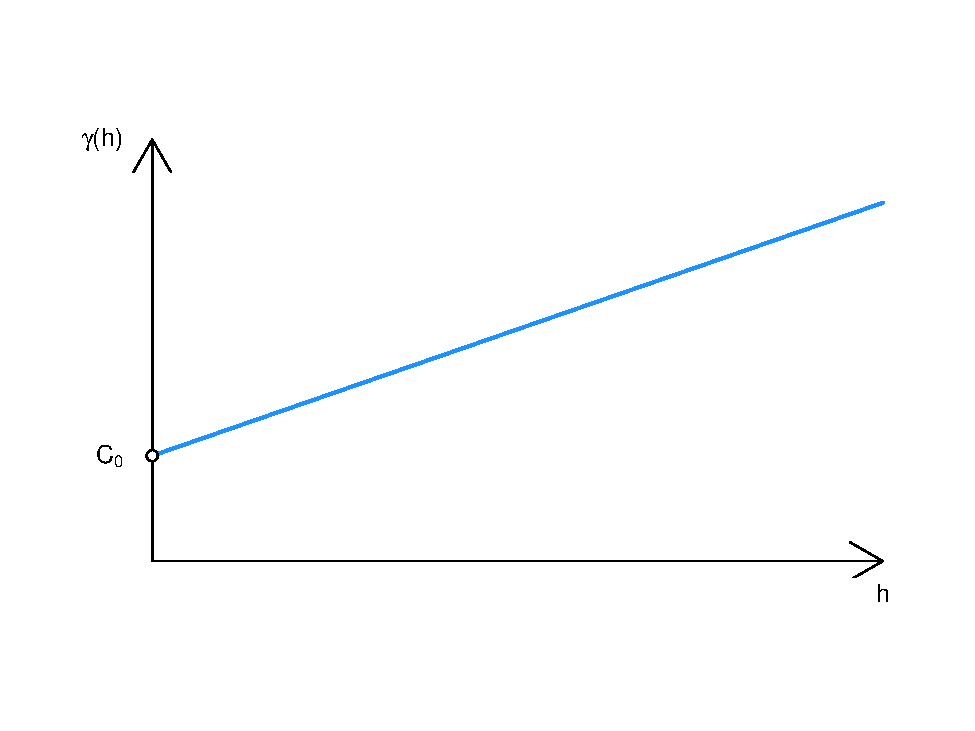
\includegraphics[width=0.7\linewidth]{Field-Trial-Spatial-Analysis-Guide_files/figure-latex/linear-CE-fig-1} 

}

\caption{Linear Error Model}\label{fig:linear-CE-fig}
\end{figure}

There is no sill or range in the linear model, so the variance will continue to increase as a function of distance.

\hypertarget{power}{%
\subsubsection{Power}\label{power}}

\[ \gamma (h)=\left\{ {\begin{array}{cc} 0 & h = 0\\ C_0+C_1h^\lambda & h > 0 \end{array} } \right. \]
where

\[ 0 \leq \lambda <\leq 2 \\ C_0 = nugget \\ C_1 = scaling \: factor \]

\begin{figure}

{\centering 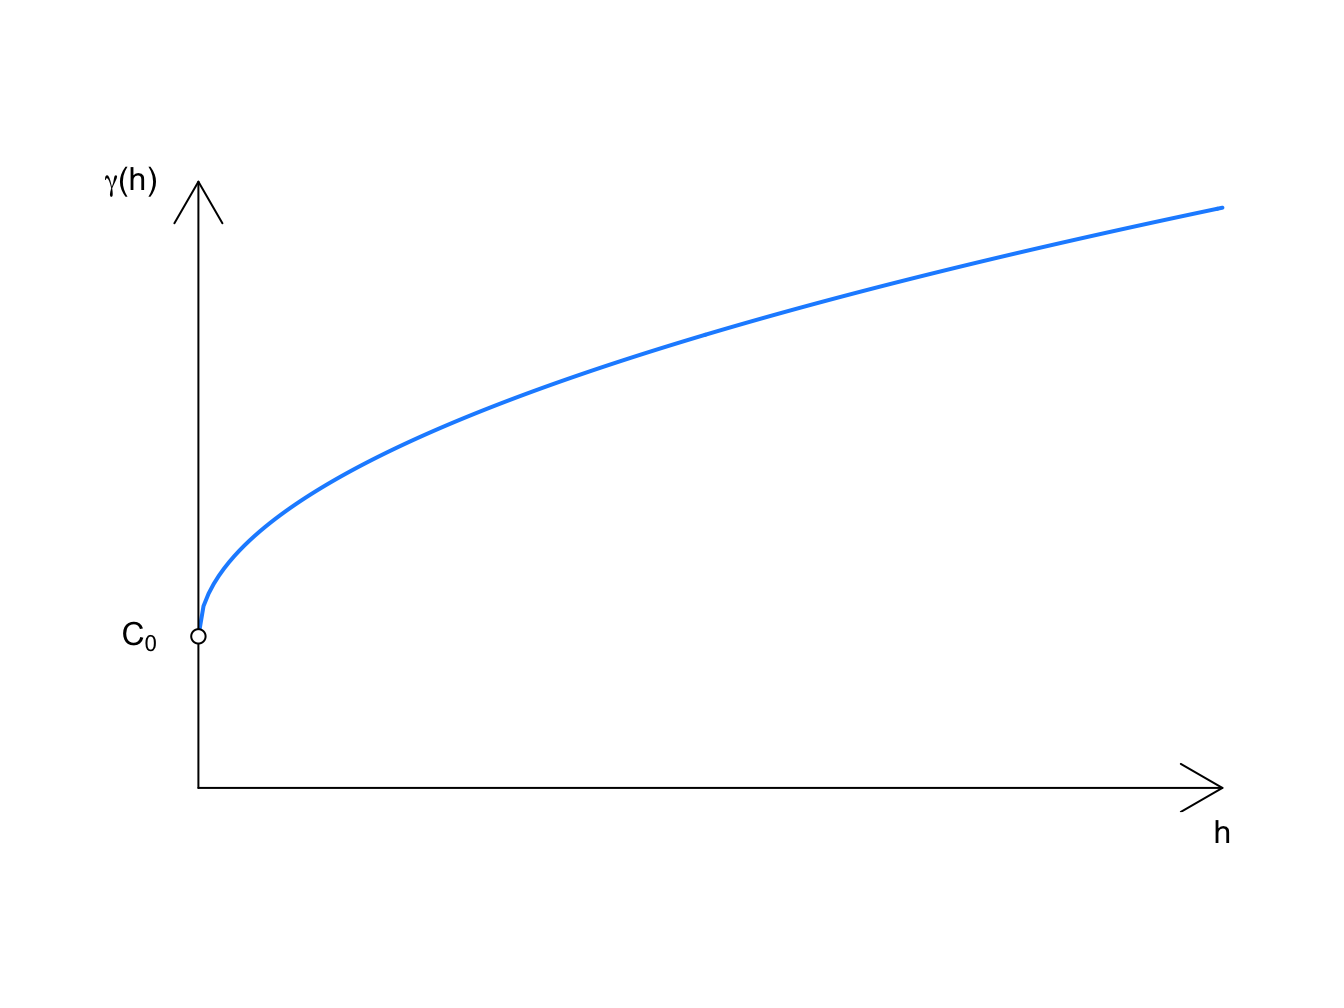
\includegraphics[width=0.7\linewidth]{Field-Trial-Spatial-Analysis-Guide_files/figure-latex/power-CE-fig-1} 

}

\caption{Power Model}\label{fig:power-CE-fig}
\end{figure}

When \(\lambda = 1\), that is equivalent to the linear model. Example above is when \(\lambda = 0.5\) (i.e.~a square-root transformation) and \(C_1 = 1\). There is also no sill or range in the power model.

\hypertarget{matuxe9rn}{%
\subsubsection{Matérn}\label{matuxe9rn}}

\[\gamma(h) = c_0 + c_1 \bigg( 1- \frac{1}{2^{\kappa -1}\Gamma(\kappa)}
\Big( \frac{h}{\alpha} \Big) ^{\kappa} K_\kappa
\Big( \frac{h}{\alpha} \Big) \bigg)\]

Where

\[ C_0 = nugget \\ C_1 = partial \: scale \\ 
\alpha = smoothing \: factor \\ \kappa = covariance \: parameter
\]

\(\Gamma(\kappa)\) is the gamma function:

\[\Gamma(\kappa) = (\kappa -1)!\]

and \(\kappa(\alpha)\) is a modified bessel function:

\[ K_\kappa(t) = \frac{\Gamma(\alpha)}{2} \big( \frac{t}{2} \big) ^{-\kappa}\]

\hypertarget{correlated-error-model-for-gridded-data}{%
\subsection{Correlated error model for gridded data}\label{correlated-error-model-for-gridded-data}}

Planned field experiments often have the advantage of being arranged in regular grid pattern that can be adequately described using Euclidean space. This simplifies aspects of understanding how error terms are related by distance since the data occur in evenly spaced increments. Furthermore, in many agricultural trials, there may be no interest in spatial interpolation between units. Some of the following models work with irregularly-spaced data, but the models below are simplified forms when the experimental units are arranged in regular grid.

For example, imagine an experiment consisting of 8 plots (plot = the experiment units) arranged in 2 rows, each with 4 ranges with this layout:

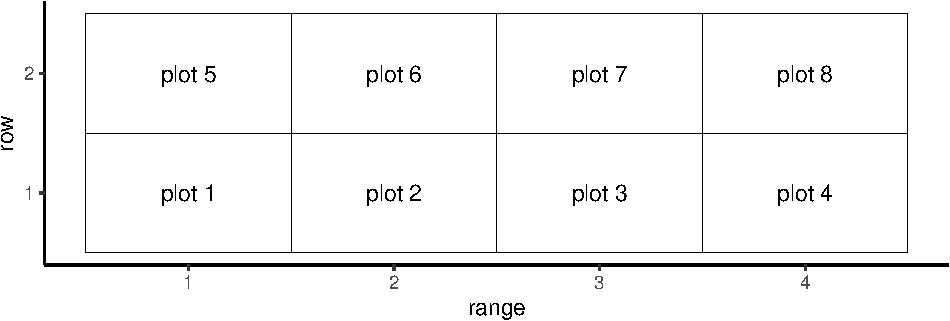
\includegraphics{Field-Trial-Spatial-Analysis-Guide_files/figure-latex/plot-grid-fig-1.pdf}

The statistical model for that experiment:

\[ 
\left[ {\begin{array} \ Y_1 \\ Y_2 \\ \vdots \\ Y_n \end{array} } \right] = \beta_0 + 
\left[ {\begin{array} \ X_1 \\ X_2 \\ \vdots \\ X_n \end{array} } \right] \beta_1 +
\left[ {\begin{array} \ \epsilon_1 \\ \epsilon_2 \\ \vdots \\ \epsilon_n \end{array} } \right]
\]
\(X\beta\) refer to independent variable effects. This same model is also often presented in an abbreviated matrix form:

\[ \mathbf{Y = X\beta + \epsilon}\]

\hypertarget{first-order-auto-regressive-model-ar1}{%
\subsubsection{First order auto-regressive model (AR1)}\label{first-order-auto-regressive-model-ar1}}

This assumes that variance can be modelled as exponential function based on unit distance (e.g.~row or range), either in a single direction or anistropic.

The AR1 structure across 2 rows is modeled as thus:

\[\mathbf { V_{AR(1)row}}  = \sigma^2
\left[ {\begin{array}{cc} 
1 & \rho \\
\rho & 1 
\end{array} } \right] \otimes \mathbf{I_4}\]

This covariance model describes the correlation of observations in the \emph{row direction only.}

And similarly the AR1 structure across 4 ranges is modeled as thus:

\[ \mathbf {V_{AR(1)range}} = \sigma^2 \mathbf{I_4} 
\left[ {\begin{array}{cccc} 
1 & \rho & \rho^2 & \rho^3 \\
\rho & 1 & \rho & \rho^2  \\
\rho^2 & \rho & 1 & \rho  \\
\rho^3 & \rho^2 & \rho & 1
\end{array} } \right] \otimes \mathbf{I_2} \]

This covariance model describes the correlation of observations in the \emph{range direction only.}

In combined AR1xAR1 model, the parameter, \(\rho\) may need to estimated separated across the row and column directions depending on the shape of the plots and site-specific field variation. Very rectangular plots are likely to require a separate estimate of the \(\rho\) parameter for each direction.

\begin{equation}
\mathbf {V_{AR(1)row} \otimes V_{AR(1)range}} = \sigma^2
\left[ {\begin{array}{cccc | cccc} 

1 & \rho_1 & \rho_1^2 & \rho_1^3 & \rho_2 & \rho_1\rho_2 & \rho_1^2\rho_2 & \rho_1^3\rho_2 \\
\rho_1 & 1 & \rho_1 & \rho_1^2 & \rho_1\rho_2 & \rho_2 & \rho_1\rho_2 & \rho_1^2\rho_2\\
\rho_1^2 & \rho_1 & 1 & \rho_1 & \rho_1^2\rho_2 & \rho_1\rho_2 & \rho_2 & \rho_1\rho_2\\
\rho_1^3 & \rho_1^2 & \rho_1 & 1 & \rho_1^3\rho_2 & \rho_1^2\rho_2 & \rho_1\rho_2 & \rho_2 \\
\hline
\rho_2 & \rho_1\rho_2 & \rho_1^2\rho_2 & \rho_1^3\rho_2 & 1 & \rho_1 & \rho_1^2 & \rho_1^3 \\
\rho_1\rho_2 & \rho_2 & \rho_1\rho_2 & \rho_1^2\rho_2 & \rho_1 & 1 & \rho_1 & \rho_1^2 \\
\rho_1^2\rho_2 & \rho_1\rho_2 & \rho_2 & \rho_1\rho_2 & \rho_1^2 & \rho_1 & 1 & \rho_1 \\
\rho_1^3\rho_2 & \rho_1^2\rho_2 & \rho_1\rho_2 & \rho_2 &\rho_1^3 & \rho_1^2 & \rho_1 & 1 \\

\end{array} } \right]
\end{equation}

\textbf{Note}: \(\rho_1\) and \(\rho_2\) are the parameter estimate for \(V_{AR1(1) row}\) and \(V_{AR(1)range}\), respectively.

Please note that these error models are for modelling localised variation based on physical proximity. It is assumed that eventually a distance in the experiment can be reached in which 2 observations can be treated independent.

If there are spatial trends that extend along the entire scope of an experiment (for instance, due to position on a slope), then an additional trend analysis should be conducted.

\hypertarget{spatial-regression-methods}{%
\section{Spatial Regression methods}\label{spatial-regression-methods}}

These approaches look use information from adjacent plots to adjust for spatial auto-correlation.

\hypertarget{spatial-autoregressive-sar}{%
\subsection{Spatial autoregressive (SAR)}\label{spatial-autoregressive-sar}}

Sometimes called a ``lag'' model, the SAR model uses correlations with neighboring plots dependent variable to predict Y. The auto-regressive model explicitly models correlations between neighboring points.

\[\mathbf{Y =  \rho W Y + X\beta + \epsilon} \]

While this may look strange, \(\mathbf{W}\) is an \(n\) x \(n\) matrix weighting the neighbors with a diagonal of zero so the value at \(i=j\), that is \(Y_{ijk}\) itself, is not used on the right-hand side to predict \(Y_{ijk}\) on the left-hand side of the equation. The error terms are assumed iid.

\textbf{On Weights}

Setting weights of neighbors is dealt with in the next chapter \ref{rcbd-r}.

\hypertarget{trend-analysis}{%
\section{Trend analysis}\label{trend-analysis}}

\hypertarget{row-and-column-trends}{%
\subsection{Row and column trends}\label{row-and-column-trends}}

Experiment wide-trends should be modeled with directional trend models. These are comparatively simple models:

\[Y_{ijk} = \beta_0 + X_{i1}\beta_1 +  Row_{j2}\beta_2 + Range_{k3}\beta_3 +\epsilon_{ijk}\]

If the assumption of independent, normal, and identical errors are met, then this model will suffice. If spatial variation is still present, additional measures will need to be taken.

\hypertarget{splines}{%
\subsection{Splines}\label{splines}}

There is a rich field of research on using localised splines to model field heterogeneity. They are similar to trend models where the row and/or column trends are modelled. These models are complex and hence not described here.

\hypertarget{spatial-r}{%
\chapter{Identifying Spatial Variation: R}\label{spatial-r}}

\hypertarget{load-data}{%
\section{Load data}\label{load-data}}

This tutorial uses the Nebraska Interstate wheat trials, first published by Stroup et al in 1994 \citep{stroup1994} and reused extensively in field spatial variation studies.

\begin{Shaded}
\begin{Highlighting}[]
\FunctionTok{library}\NormalTok{(agridat); }\FunctionTok{library}\NormalTok{(dplyr); }\FunctionTok{library}\NormalTok{(tidyr)}

\FunctionTok{data}\NormalTok{(}\StringTok{"stroup.nin"}\NormalTok{)}

\NormalTok{Nin }\OtherTok{\textless{}{-}}\NormalTok{ stroup.nin }\SpecialCharTok{\%\textgreater{}\%} \FunctionTok{mutate}\NormalTok{(}\AttributeTok{col.width =}\NormalTok{ col }\SpecialCharTok{*} \FloatTok{1.2}\NormalTok{, }
                             \AttributeTok{row.length =}\NormalTok{ row }\SpecialCharTok{*} \FloatTok{4.3}\NormalTok{) }\SpecialCharTok{\%\textgreater{}\%} 
  \FunctionTok{mutate}\NormalTok{(}\AttributeTok{name =} \FunctionTok{case\_when}\NormalTok{(}\FunctionTok{is.na}\NormalTok{(}\FunctionTok{as.character}\NormalTok{(rep)) }\SpecialCharTok{\textasciitilde{}} \ConstantTok{NA\_character\_}\NormalTok{, }
                          \ConstantTok{TRUE} \SpecialCharTok{\textasciitilde{}} \FunctionTok{as.character}\NormalTok{(gen))) }\SpecialCharTok{\%\textgreater{}\%} 
  \FunctionTok{arrange}\NormalTok{(col, row)}

\NormalTok{Nin\_na }\OtherTok{\textless{}{-}} \FunctionTok{filter}\NormalTok{(Nin, }\SpecialCharTok{!}\FunctionTok{is.na}\NormalTok{(rep))}
\end{Highlighting}
\end{Shaded}

\hypertarget{examine-data}{%
\subsection{Examine data}\label{examine-data}}

\begin{Shaded}
\begin{Highlighting}[]
\FunctionTok{head}\NormalTok{(Nin)}
\end{Highlighting}
\end{Shaded}

\begin{verbatim}
##        gen  rep yield col row col.width row.length     name
## 1   Lancer <NA>    NA   1   1       1.2        4.3     <NA>
## 2  NE83407   R1 19.40   1   2       1.2        8.6  NE83407
## 3 Buckskin   R1 29.85   1   3       1.2       12.9 Buckskin
## 4  NE87612   R1 28.15   1   4       1.2       17.2  NE87612
## 5     Vona   R2 26.80   1   5       1.2       21.5     Vona
## 6  NE87512   R2 20.20   1   6       1.2       25.8  NE87512
\end{verbatim}

This data set actually has no missing data -- this is a balanced trial. However, there are empty fill plot with no data which creates some issues regarding NA handling.

Plot raw yield data as it appeared in the field:

\begin{Shaded}
\begin{Highlighting}[]
\FunctionTok{library}\NormalTok{(ggplot2); }\FunctionTok{library}\NormalTok{(desplot)}
\end{Highlighting}
\end{Shaded}

\begin{Shaded}
\begin{Highlighting}[]
\FunctionTok{ggplot}\NormalTok{(Nin, }\FunctionTok{aes}\NormalTok{(}\AttributeTok{x =}\NormalTok{ row, }\AttributeTok{y =}\NormalTok{ col)) }\SpecialCharTok{+}
  \FunctionTok{geom\_tile}\NormalTok{(}\FunctionTok{aes}\NormalTok{(}\AttributeTok{fill =}\NormalTok{ yield), }\AttributeTok{col =} \StringTok{"white"}\NormalTok{) }\SpecialCharTok{+}
  \CommentTok{\#geom\_text(aes(label = name)) +}
  \FunctionTok{geom\_tileborder}\NormalTok{(}\FunctionTok{aes}\NormalTok{(}\AttributeTok{group =} \DecValTok{1}\NormalTok{, }\AttributeTok{grp =}\NormalTok{ rep), }\AttributeTok{lwd =} \FloatTok{1.2}\NormalTok{) }\SpecialCharTok{+}
  \FunctionTok{scale\_fill\_gradient}\NormalTok{(}\AttributeTok{low =} \StringTok{"white"}\NormalTok{, }\AttributeTok{high =} \StringTok{"blue"}\NormalTok{) }\SpecialCharTok{+}
  \FunctionTok{scale\_x\_continuous}\NormalTok{(}\AttributeTok{breaks =} \FunctionTok{seq}\NormalTok{(}\DecValTok{1}\NormalTok{,}\FunctionTok{max}\NormalTok{(Nin}\SpecialCharTok{$}\NormalTok{row), }\DecValTok{1}\NormalTok{)) }\SpecialCharTok{+}
  \FunctionTok{scale\_y\_continuous}\NormalTok{(}\AttributeTok{breaks =} \DecValTok{1}\SpecialCharTok{:}\FunctionTok{max}\NormalTok{(Nin}\SpecialCharTok{$}\NormalTok{col)) }\SpecialCharTok{+}
  \FunctionTok{labs}\NormalTok{(}\AttributeTok{x =} \StringTok{"row"}\NormalTok{, }\AttributeTok{y =} \StringTok{"column"}\NormalTok{, }\AttributeTok{title =} \StringTok{"field plot layout"}\NormalTok{) }\SpecialCharTok{+} 
  \FunctionTok{theme\_classic}\NormalTok{() }\SpecialCharTok{+}
  \FunctionTok{theme}\NormalTok{(}\AttributeTok{axis.text =} \FunctionTok{element\_text}\NormalTok{(}\AttributeTok{size =} \DecValTok{12}\NormalTok{),}
        \AttributeTok{axis.title =} \FunctionTok{element\_text}\NormalTok{(}\AttributeTok{size =} \DecValTok{14}\NormalTok{),}
        \AttributeTok{legend.title =} \FunctionTok{element\_text}\NormalTok{(}\AttributeTok{size =} \DecValTok{14}\NormalTok{),}
        \AttributeTok{legend.text =} \FunctionTok{element\_text}\NormalTok{(}\AttributeTok{size =} \DecValTok{12}\NormalTok{))}
\end{Highlighting}
\end{Shaded}

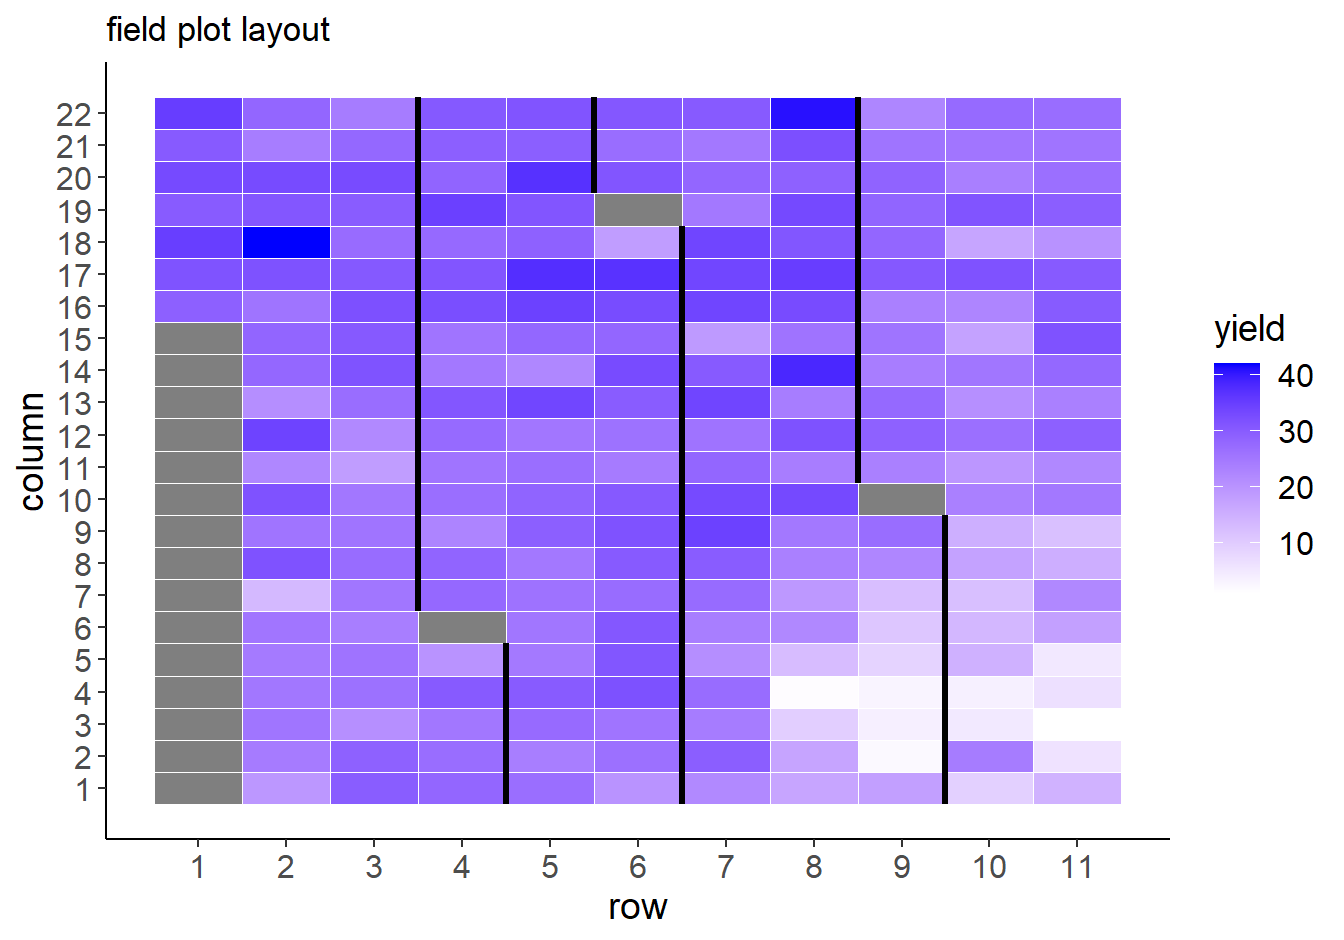
\includegraphics[width=1\linewidth]{Field-Trial-Spatial-Analysis-Guide_files/figure-latex/Nin-yield-layout-fig-1}

Black lines delineate the blocks.

It's also helpful to plot raw response data:

\begin{Shaded}
\begin{Highlighting}[]
\FunctionTok{par}\NormalTok{(}\AttributeTok{mfrow=}\FunctionTok{c}\NormalTok{(}\DecValTok{1}\NormalTok{,}\DecValTok{3}\NormalTok{))}
\FunctionTok{boxplot}\NormalTok{(yield }\SpecialCharTok{\textasciitilde{}}\NormalTok{ rep, }\AttributeTok{data =}\NormalTok{ Nin, }\AttributeTok{xlab =} \StringTok{"rep"}\NormalTok{, }\AttributeTok{ylab =} \StringTok{"yield (bu/acres)"}\NormalTok{, }\AttributeTok{col =} \StringTok{"red2"}\NormalTok{, }\AttributeTok{main =} \StringTok{"yield across blocks"}\NormalTok{)}
\FunctionTok{boxplot}\NormalTok{(yield }\SpecialCharTok{\textasciitilde{}}\NormalTok{ row, }\AttributeTok{data =}\NormalTok{ Nin, }\AttributeTok{xlab =} \StringTok{"row"}\NormalTok{, }\AttributeTok{ylab =} \StringTok{"yield (bu/acres)"}\NormalTok{,}\AttributeTok{col =} \StringTok{"dodgerblue2"}\NormalTok{, }\AttributeTok{main =} \StringTok{"yield across rows"}\NormalTok{)}
\FunctionTok{boxplot}\NormalTok{(yield }\SpecialCharTok{\textasciitilde{}}\NormalTok{ col, }\AttributeTok{data =}\NormalTok{ Nin, }\AttributeTok{col =} \StringTok{"gold"}\NormalTok{, }\AttributeTok{xlab =} \StringTok{"column"}\NormalTok{, }\AttributeTok{ylab =} \StringTok{"yield (bu/acres)"}\NormalTok{,}\AttributeTok{main =} \StringTok{"yield across columns"}\NormalTok{)}
\end{Highlighting}
\end{Shaded}

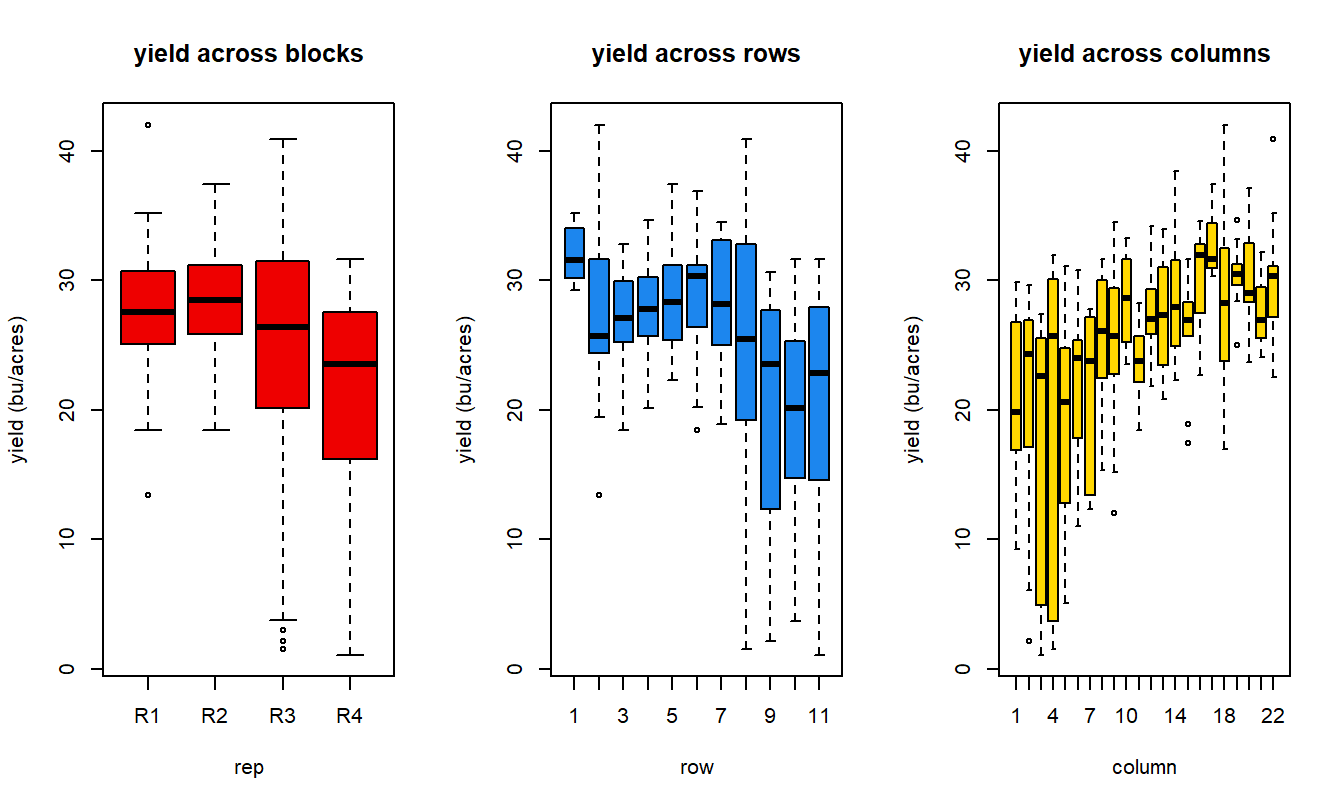
\includegraphics[width=0.8\linewidth]{Field-Trial-Spatial-Analysis-Guide_files/figure-latex/Nin-boxplot-fig-1}

\begin{Shaded}
\begin{Highlighting}[]
\FunctionTok{par}\NormalTok{(}\AttributeTok{mfrow=}\FunctionTok{c}\NormalTok{(}\DecValTok{1}\NormalTok{,}\DecValTok{1}\NormalTok{))}
\end{Highlighting}
\end{Shaded}

\hypertarget{test-for-spatial-autocorrelation}{%
\section{Test for spatial autocorrelation}\label{test-for-spatial-autocorrelation}}

\hypertarget{morans-i-1}{%
\subsection{Moran's I}\label{morans-i-1}}

First, run a standard linear model of the experiment:

\begin{Shaded}
\begin{Highlighting}[]
\FunctionTok{library}\NormalTok{(nlme)}

\NormalTok{nin.lme }\OtherTok{\textless{}{-}} \FunctionTok{lme}\NormalTok{(yield }\SpecialCharTok{\textasciitilde{}}\NormalTok{ gen, }\AttributeTok{random =} \SpecialCharTok{\textasciitilde{}}\DecValTok{1}\SpecialCharTok{|}\NormalTok{rep,}
              \AttributeTok{data =}\NormalTok{ Nin,}
              \AttributeTok{na.action =}\NormalTok{ na.exclude)}
\end{Highlighting}
\end{Shaded}

Next, establish and weight neighbors for each plot. In this example, only adjacent neighbors in the rook formation (see \ref{background}) are used and are weighted proportionally according to their representation as neighbors to an individual. That is, if a unit has 4 adjacent neighbors, each neighbor is weighted as 0.25. If there are only two neighbors, each is weighted 0.5.

The function \texttt{cell2nb()} is a function for setting neighbors when working with data laid out in a regular grid.

\begin{Shaded}
\begin{Highlighting}[]
\FunctionTok{library}\NormalTok{(spdep)}
\NormalTok{xy\_rook }\OtherTok{\textless{}{-}} \FunctionTok{cell2nb}\NormalTok{(}\AttributeTok{nrow =} \FunctionTok{max}\NormalTok{(Nin}\SpecialCharTok{$}\NormalTok{row), }\AttributeTok{ncol =} \FunctionTok{max}\NormalTok{(Nin}\SpecialCharTok{$}\NormalTok{col), }\AttributeTok{type=}\StringTok{"rook"}\NormalTok{, }\AttributeTok{torus =} \ConstantTok{FALSE}\NormalTok{, }\AttributeTok{legacy =} \ConstantTok{FALSE}\NormalTok{)  }
\end{Highlighting}
\end{Shaded}

\textbf{Make sure your data sorted by the variables assigned to row and col (in that order), and there is one and only one observation in the data set for each unique row/col combination. Even missing plots need a row.}

\emph{Rook adjacency plot for the NIN data}

\begin{Shaded}
\begin{Highlighting}[]
\FunctionTok{library}\NormalTok{(sf)}
\NormalTok{rook\_matrix }\OtherTok{\textless{}{-}} \FunctionTok{st\_as\_sf}\NormalTok{(}\FunctionTok{expand.grid}\NormalTok{(}\AttributeTok{col=}\DecValTok{1}\SpecialCharTok{:}\DecValTok{22}\NormalTok{, }\AttributeTok{row=}\DecValTok{1}\SpecialCharTok{:}\DecValTok{11}\NormalTok{), }\AttributeTok{coords=}\FunctionTok{c}\NormalTok{(}\StringTok{"col"}\NormalTok{, }\StringTok{"row"}\NormalTok{))}
\FunctionTok{plot}\NormalTok{(xy\_rook, }\AttributeTok{coords =} \FunctionTok{st\_geometry}\NormalTok{(rook\_matrix), }\AttributeTok{points =} \ConstantTok{TRUE}\NormalTok{)}
\end{Highlighting}
\end{Shaded}

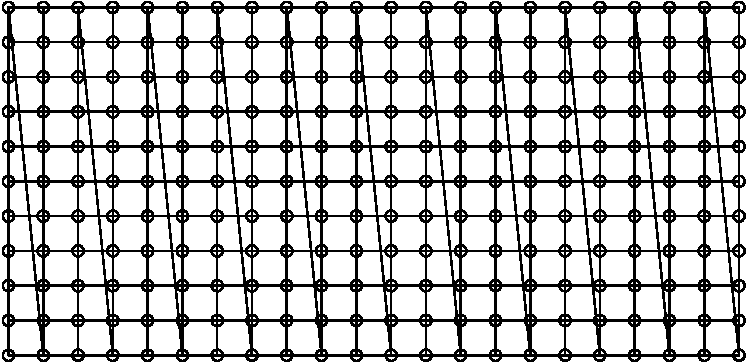
\includegraphics{Field-Trial-Spatial-Analysis-Guide_files/figure-latex/nin-rook-adj-fg-1.pdf}
Each observation considers ``neighbors'' to be those which touch the cell in a row or column orientation, but not diagonal.

Conduct Moran's test via standard t-test and using MC sampling.

\begin{Shaded}
\begin{Highlighting}[]
\NormalTok{resid\_lme }\OtherTok{\textless{}{-}} \FunctionTok{residuals}\NormalTok{(nin.lme)}
\FunctionTok{names}\NormalTok{(resid\_lme) }\OtherTok{\textless{}{-}}\NormalTok{ Nin}\SpecialCharTok{$}\NormalTok{plot}
\FunctionTok{moran.test}\NormalTok{(resid\_lme, }\FunctionTok{nb2listw}\NormalTok{(xy\_rook), }\AttributeTok{na.action =}\NormalTok{ na.exclude)}
\end{Highlighting}
\end{Shaded}

\begin{verbatim}
## 
##  Moran I test under randomisation
## 
## data:  resid_lme  
## weights: nb2listw(xy_rook) 
## omitted: 1, 12, 23, 34, 45, 56, 59, 67, 78, 89, 100, 108, 111, 122, 133, 144, 155, 204   
## 
## Moran I statistic standard deviate = 8.1602, p-value < 2.2e-16
## alternative hypothesis: greater
## sample estimates:
## Moran I statistic       Expectation          Variance 
##       0.402504491      -0.004484305       0.002487522
\end{verbatim}

\begin{Shaded}
\begin{Highlighting}[]
\FunctionTok{moran.mc}\NormalTok{(resid\_lme, }\FunctionTok{nb2listw}\NormalTok{(xy\_rook), }\DecValTok{999}\NormalTok{, }\AttributeTok{na.action =}\NormalTok{ na.exclude)}
\end{Highlighting}
\end{Shaded}

\begin{verbatim}
## 
##  Monte-Carlo simulation of Moran I
## 
## data:  resid_lme 
## weights: nb2listw(xy_rook) 
## omitted: 1, 12, 23, 34, 45, 56, 59, 67, 78, 89, 100, 108, 111, 122, 133, 144, 155, 204 
## number of simulations + 1: 1000 
## 
## statistic = 0.4025, observed rank = 1000, p-value = 0.001
## alternative hypothesis: greater
\end{verbatim}

Plot Spatial dependence of residuals

\begin{Shaded}
\begin{Highlighting}[]
\FunctionTok{library}\NormalTok{(purrr)}

\NormalTok{res.nn1 }\OtherTok{\textless{}{-}} \FunctionTok{map\_dbl}\NormalTok{(xy\_rook, }\ControlFlowTok{function}\NormalTok{(j) }\FunctionTok{mean}\NormalTok{(resid\_lme[j]))}
  
\NormalTok{rc }\OtherTok{\textless{}{-}} \FunctionTok{signif}\NormalTok{(}\FunctionTok{cor}\NormalTok{(resid\_lme, res.nn1, }\AttributeTok{use =} \StringTok{"pairwise.complete.obs"}\NormalTok{), }\DecValTok{2}\NormalTok{)}

\FunctionTok{plot}\NormalTok{(}\AttributeTok{x =}\NormalTok{ resid\_lme, }\AttributeTok{y =}\NormalTok{ res.nn1, }
     \AttributeTok{main =} \FunctionTok{paste0}\NormalTok{(}\StringTok{"r = "}\NormalTok{, rc), }\AttributeTok{xlab =} \StringTok{"residual"}\NormalTok{, }\AttributeTok{ylab =} \StringTok{"average residual of neighbor (rook)"}\NormalTok{)}
\end{Highlighting}
\end{Shaded}

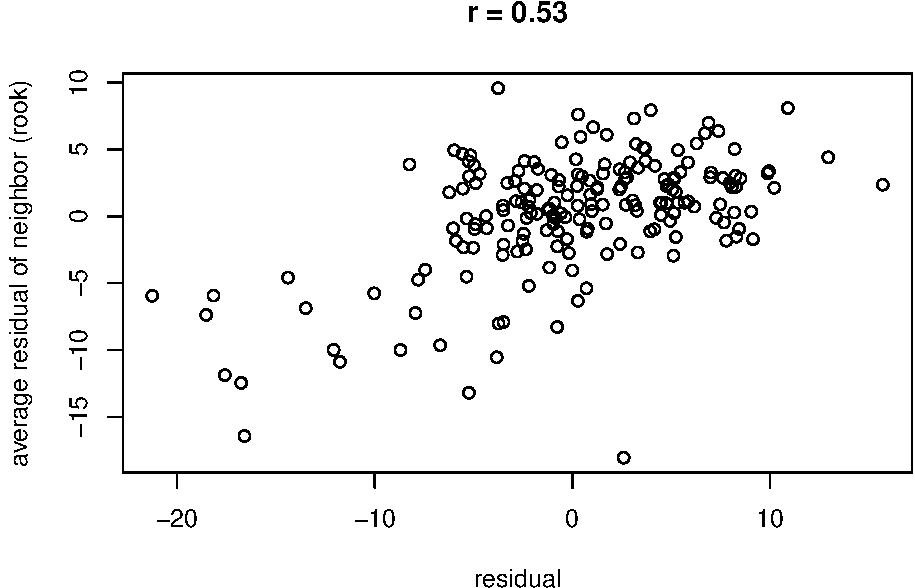
\includegraphics{Field-Trial-Spatial-Analysis-Guide_files/figure-latex/resid-cor-fig-1.pdf}

\hypertarget{note-on-gearys-c}{%
\subsection{Note on Geary's C}\label{note-on-gearys-c}}

At this time, the \textbf{spdep} function \texttt{geary.test()} for Geary's C does not handle missing spatial points. It cannot be used it for the NIN data set because it contains empty plots between each block with no data available for those plots.

\hypertarget{empirical-variogram-fitting}{%
\section{Empirical variogram fitting}\label{empirical-variogram-fitting}}

First, create a spatial object by adding spatial coordinates to an ordinary data frame. I like to use the actual size of the plots since they are often exaggerated rectangles that have a significantly greater length than width.

\begin{Shaded}
\begin{Highlighting}[]
\FunctionTok{library}\NormalTok{(sp)}
\end{Highlighting}
\end{Shaded}

\begin{verbatim}
## Warning: package 'sp' was built under R version 4.3.1
\end{verbatim}

\begin{Shaded}
\begin{Highlighting}[]
\NormalTok{Nin\_spatial }\OtherTok{\textless{}{-}}\NormalTok{ Nin\_na}
\FunctionTok{coordinates}\NormalTok{(Nin\_spatial) }\OtherTok{\textless{}{-}} \ErrorTok{\textasciitilde{}}\NormalTok{ col.width }\SpecialCharTok{+}\NormalTok{ row.length}
\FunctionTok{class}\NormalTok{(Nin\_spatial)}
\end{Highlighting}
\end{Shaded}

\begin{verbatim}
## [1] "SpatialPointsDataFrame"
## attr(,"package")
## [1] "sp"
\end{verbatim}

Set the maximum distance for calculating the variogram model (which is one-half the maximum distance between two points).

\begin{Shaded}
\begin{Highlighting}[]
\NormalTok{max\_dist }\OtherTok{=} \FloatTok{0.6}\SpecialCharTok{*}\FunctionTok{max}\NormalTok{(}\FunctionTok{dist}\NormalTok{(}\FunctionTok{coordinates}\NormalTok{(Nin\_spatial)))}
\FunctionTok{round}\NormalTok{(max\_dist, }\AttributeTok{digits =} \DecValTok{2}\NormalTok{)}
\end{Highlighting}
\end{Shaded}

\begin{verbatim}
## [1] 29.9
\end{verbatim}

Calculate semivariance for an isotropic model and plot the variogram.

\begin{Shaded}
\begin{Highlighting}[]
\FunctionTok{library}\NormalTok{(gstat)}
\end{Highlighting}
\end{Shaded}

\begin{verbatim}
## Warning: package 'gstat' was built under R version 4.3.1
\end{verbatim}

\begin{Shaded}
\begin{Highlighting}[]
\FunctionTok{class}\NormalTok{(Nin\_spatial)}
\end{Highlighting}
\end{Shaded}

\begin{verbatim}
## [1] "SpatialPointsDataFrame"
## attr(,"package")
## [1] "sp"
\end{verbatim}

\begin{Shaded}
\begin{Highlighting}[]
\FunctionTok{head}\NormalTok{(Nin\_spatial)}
\end{Highlighting}
\end{Shaded}

\begin{verbatim}
##   coordinates      gen rep yield col row     name
## 1  (1.2, 8.6)  NE83407  R1 19.40   1   2  NE83407
## 2 (1.2, 12.9) Buckskin  R1 29.85   1   3 Buckskin
## 3 (1.2, 17.2)  NE87612  R1 28.15   1   4  NE87612
## 4 (1.2, 21.5)     Vona  R2 26.80   1   5     Vona
## 5 (1.2, 25.8)  NE87512  R2 20.20   1   6  NE87512
## 6 (1.2, 30.1)  NE87408  R3 21.90   1   7  NE87408
\end{verbatim}

\begin{Shaded}
\begin{Highlighting}[]
\NormalTok{resid\_var1 }\OtherTok{\textless{}{-}}\NormalTok{ gstat}\SpecialCharTok{::}\FunctionTok{variogram}\NormalTok{(yield }\SpecialCharTok{\textasciitilde{}}\NormalTok{ rep }\SpecialCharTok{+}\NormalTok{ gen, }
                        \AttributeTok{cutoff =}\NormalTok{ max\_dist,}
                        \AttributeTok{width =}\NormalTok{ max\_dist}\SpecialCharTok{/}\DecValTok{20}\NormalTok{, }\CommentTok{\# 20 is the number of bins}
                        \AttributeTok{data =}\NormalTok{ Nin\_spatial)}
\FunctionTok{plot}\NormalTok{(resid\_var1)}
\end{Highlighting}
\end{Shaded}

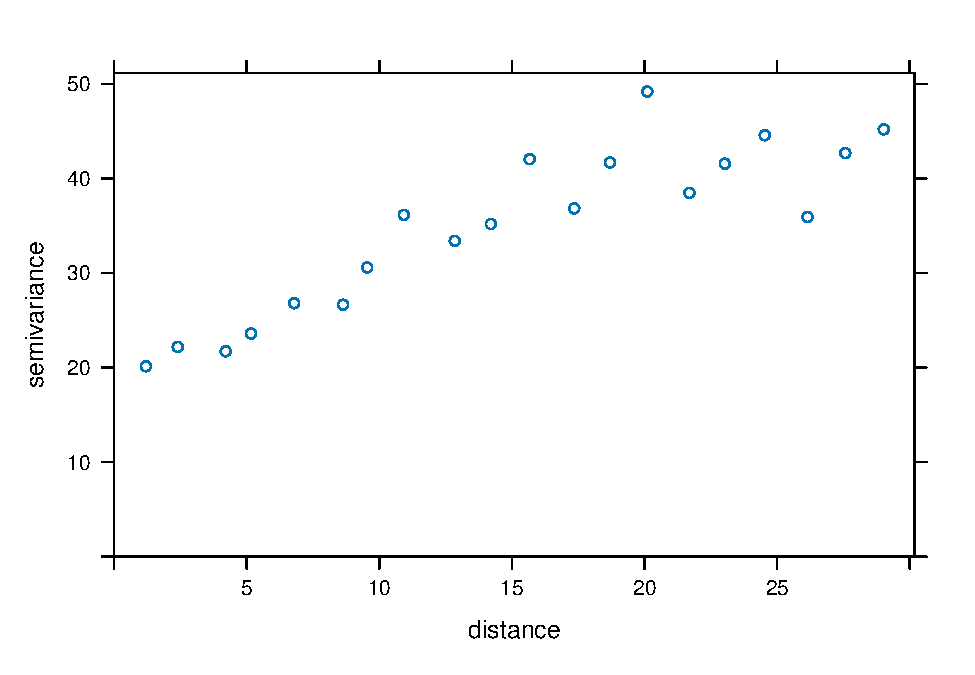
\includegraphics{Field-Trial-Spatial-Analysis-Guide_files/figure-latex/possible-error-1.pdf}

Test out correlated error models:

First, set the starting nugget values as the minimum of the semi-variance. There is likely more sophisticated methods to establish the starting value for nugget, but I have found that extracting the minimum value of the semivariance to work well as a starting point.

\begin{Shaded}
\begin{Highlighting}[]
\NormalTok{nugget\_start }\OtherTok{\textless{}{-}} \FunctionTok{min}\NormalTok{(resid\_var1}\SpecialCharTok{$}\NormalTok{gamma)}
\end{Highlighting}
\end{Shaded}

Establish models for variogram fitting.

\begin{Shaded}
\begin{Highlighting}[]
\NormalTok{Nin\_vgm1 }\OtherTok{\textless{}{-}} \FunctionTok{vgm}\NormalTok{(}\AttributeTok{model =} \StringTok{"Exp"}\NormalTok{, }\AttributeTok{nugget =}\NormalTok{ nugget\_start) }\CommentTok{\# exponential}
\NormalTok{Nin\_vgm2 }\OtherTok{\textless{}{-}} \FunctionTok{vgm}\NormalTok{(}\AttributeTok{model =} \StringTok{"Sph"}\NormalTok{, }\AttributeTok{nugget =}\NormalTok{ nugget\_start) }\CommentTok{\# spherical}
\NormalTok{Nin\_vgm3 }\OtherTok{\textless{}{-}} \FunctionTok{vgm}\NormalTok{(}\AttributeTok{model =} \StringTok{"Gau"}\NormalTok{, }\AttributeTok{nugget =}\NormalTok{ nugget\_start) }\CommentTok{\# Gaussian}
\NormalTok{Nin\_vgm4 }\OtherTok{\textless{}{-}} \FunctionTok{vgm}\NormalTok{(}\AttributeTok{model =} \StringTok{"Mat"}\NormalTok{, }\AttributeTok{nugget =}\NormalTok{ nugget\_start) }\CommentTok{\# Matern}
\end{Highlighting}
\end{Shaded}

Fit the variograms to the data:

\begin{Shaded}
\begin{Highlighting}[]
\NormalTok{Nin\_variofit1 }\OtherTok{\textless{}{-}} \FunctionTok{fit.variogram}\NormalTok{(resid\_var1, Nin\_vgm1)}
\NormalTok{Nin\_variofit2 }\OtherTok{\textless{}{-}} \FunctionTok{fit.variogram}\NormalTok{(resid\_var1, Nin\_vgm2)}
\NormalTok{Nin\_variofit3 }\OtherTok{\textless{}{-}} \FunctionTok{fit.variogram}\NormalTok{(resid\_var1, Nin\_vgm3)}
\NormalTok{Nin\_variofit4 }\OtherTok{\textless{}{-}} \FunctionTok{fit.variogram}\NormalTok{(resid\_var1, Nin\_vgm4, }\AttributeTok{fit.kappa =}\NormalTok{ T)}
\end{Highlighting}
\end{Shaded}

\hypertarget{compare-variograms}{%
\subsection{Compare variograms}\label{compare-variograms}}

Look at the results! (this is fun)

\begin{Shaded}
\begin{Highlighting}[]
\FunctionTok{plot}\NormalTok{(resid\_var1, Nin\_variofit1, }\AttributeTok{main =} \StringTok{"Exponential model"}\NormalTok{)}
\end{Highlighting}
\end{Shaded}

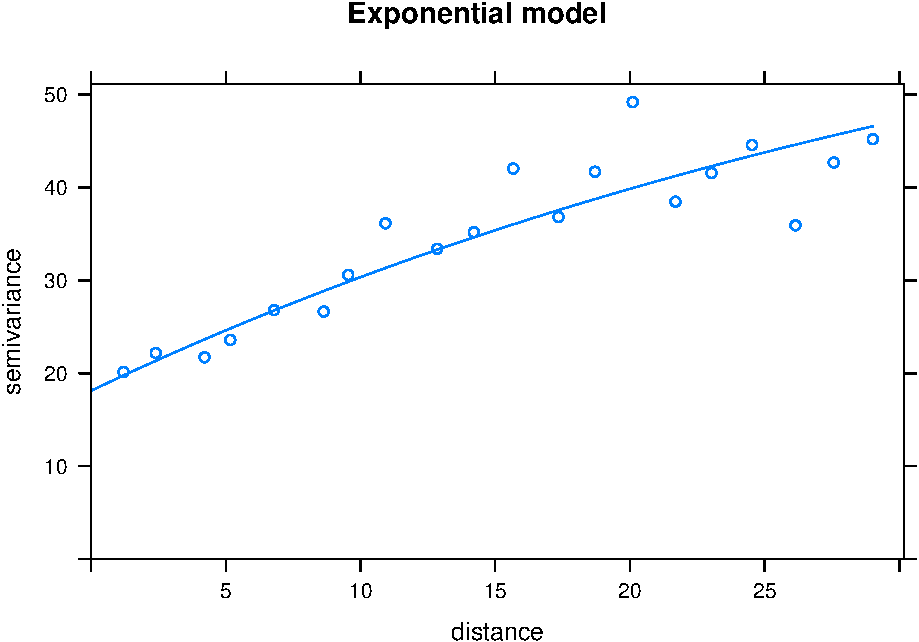
\includegraphics{Field-Trial-Spatial-Analysis-Guide_files/figure-latex/unnamed-chunk-18-1.pdf}

\begin{Shaded}
\begin{Highlighting}[]
\FunctionTok{plot}\NormalTok{(resid\_var1, Nin\_variofit2, }\AttributeTok{main =} \StringTok{"Spherical model"}\NormalTok{)}
\end{Highlighting}
\end{Shaded}

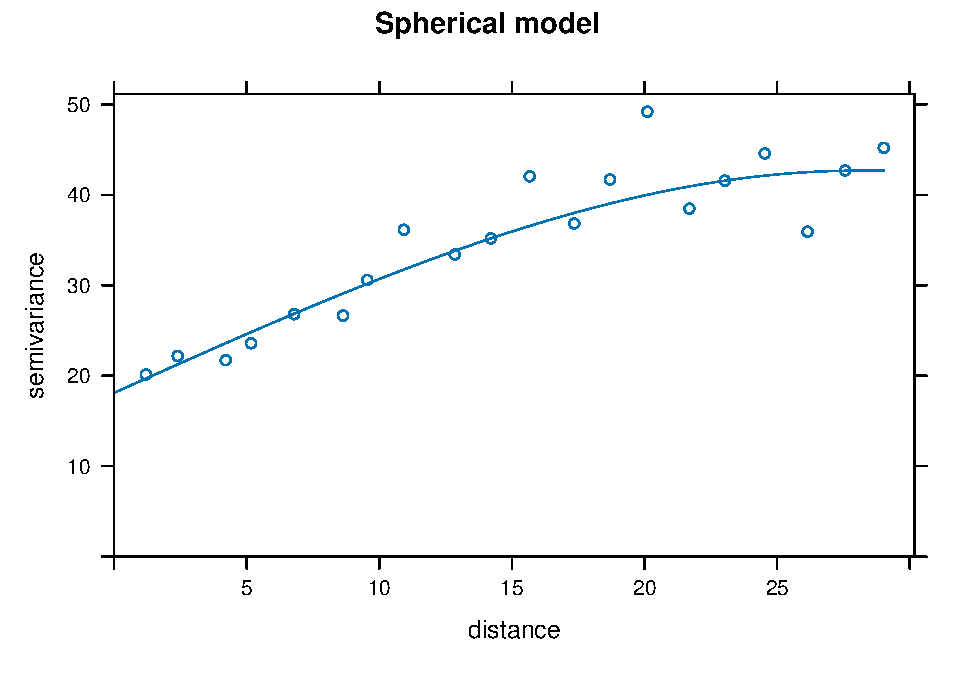
\includegraphics{Field-Trial-Spatial-Analysis-Guide_files/figure-latex/unnamed-chunk-18-2.pdf}

\begin{Shaded}
\begin{Highlighting}[]
\FunctionTok{plot}\NormalTok{(resid\_var1, Nin\_variofit3, }\AttributeTok{main =} \StringTok{"Gaussian model"}\NormalTok{)}
\end{Highlighting}
\end{Shaded}

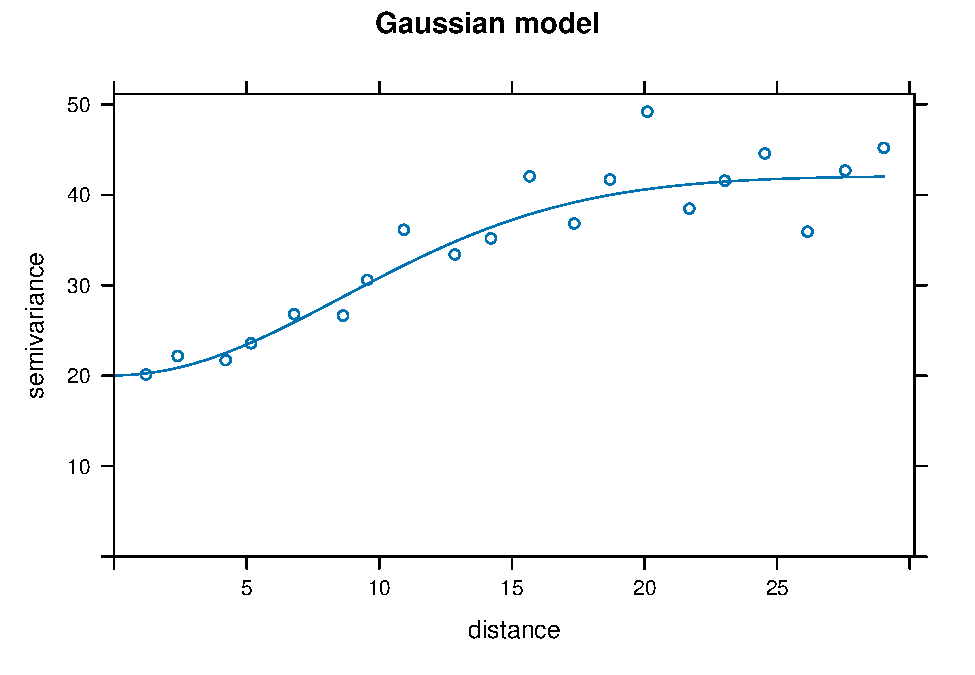
\includegraphics{Field-Trial-Spatial-Analysis-Guide_files/figure-latex/unnamed-chunk-18-3.pdf}

\begin{Shaded}
\begin{Highlighting}[]
\FunctionTok{plot}\NormalTok{(resid\_var1, Nin\_variofit4, }\AttributeTok{main =} \StringTok{"Matern model"}\NormalTok{)}
\end{Highlighting}
\end{Shaded}

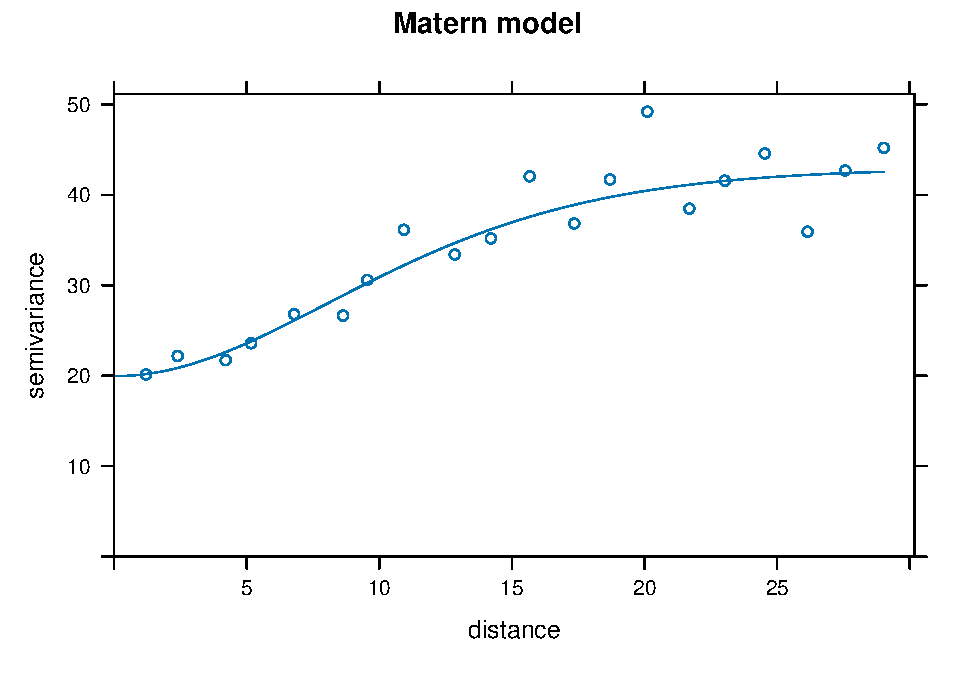
\includegraphics{Field-Trial-Spatial-Analysis-Guide_files/figure-latex/unnamed-chunk-18-4.pdf}

How to pick the best one model? The attribute ``SSError'' indicates how well each model was able to predict the binned error terms as a function of distance. However, it's important to look at the model as well to see if the model was able to fit the data.

\begin{Shaded}
\begin{Highlighting}[]
\FunctionTok{print}\NormalTok{(}\StringTok{"Exponential"}\NormalTok{); }\FunctionTok{attr}\NormalTok{(Nin\_variofit1, }\StringTok{"SSErr"}\NormalTok{)}
\end{Highlighting}
\end{Shaded}

\begin{verbatim}
## [1] "Exponential"
\end{verbatim}

\begin{verbatim}
## [1] 1129.799
\end{verbatim}

\begin{Shaded}
\begin{Highlighting}[]
\FunctionTok{print}\NormalTok{(}\StringTok{"Spherical"}\NormalTok{); }\FunctionTok{attr}\NormalTok{(Nin\_variofit2, }\StringTok{"SSErr"}\NormalTok{)}
\end{Highlighting}
\end{Shaded}

\begin{verbatim}
## [1] "Spherical"
\end{verbatim}

\begin{verbatim}
## [1] 1012.76
\end{verbatim}

\begin{Shaded}
\begin{Highlighting}[]
\FunctionTok{print}\NormalTok{(}\StringTok{"Gaussian"}\NormalTok{); }\FunctionTok{attr}\NormalTok{(Nin\_variofit3, }\StringTok{"SSErr"}\NormalTok{)}
\end{Highlighting}
\end{Shaded}

\begin{verbatim}
## [1] "Gaussian"
\end{verbatim}

\begin{verbatim}
## [1] 752.5491
\end{verbatim}

\begin{Shaded}
\begin{Highlighting}[]
\FunctionTok{print}\NormalTok{(}\StringTok{"Matern"}\NormalTok{); }\FunctionTok{attr}\NormalTok{(Nin\_variofit4, }\StringTok{"SSErr"}\NormalTok{)}
\end{Highlighting}
\end{Shaded}

\begin{verbatim}
## [1] "Matern"
\end{verbatim}

\begin{verbatim}
## [1] 771.4813
\end{verbatim}

\texttt{Nin\_variofit3} had the lowest error terms, corresponding to the Gaussian model.

Results from the empirical variogram:

\begin{Shaded}
\begin{Highlighting}[]
\NormalTok{Nin\_variofit3}
\end{Highlighting}
\end{Shaded}

\begin{verbatim}
##   model    psill    range
## 1   Nug 20.04106  0.00000
## 2   Gau 22.04013 12.19921
\end{verbatim}

The variogram parameters can be easily extracted from this table:

\begin{Shaded}
\begin{Highlighting}[]
\NormalTok{nugget }\OtherTok{\textless{}{-}}\NormalTok{ Nin\_variofit3}\SpecialCharTok{$}\NormalTok{psill[}\DecValTok{1}\NormalTok{] }\CommentTok{\# "measurement error"}
\NormalTok{range }\OtherTok{\textless{}{-}}\NormalTok{ Nin\_variofit3}\SpecialCharTok{$}\NormalTok{range[}\DecValTok{2}\NormalTok{] }\CommentTok{\# distance to establish independence between data points}
\NormalTok{sill }\OtherTok{\textless{}{-}} \FunctionTok{sum}\NormalTok{(Nin\_variofit3}\SpecialCharTok{$}\NormalTok{psill) }\CommentTok{\# maximum semivariance}
\end{Highlighting}
\end{Shaded}

\hypertarget{explore-anisotropy}{%
\subsection{Explore anisotropy}\label{explore-anisotropy}}

Most field experiments occur on a relatively small scale,where the entire experimental layout is less than 0.25 square miles. As such, isotropic models (where spatial correlation is based on distance but not direction) are often adequate for understanding localised field heterogeneity. However, there are always exceptions where a spatial correlation in a field trail is best describe by an anistropic model.

Reestablish models for variogram fitting:

\begin{Shaded}
\begin{Highlighting}[]
\NormalTok{Nin\_vgm1a }\OtherTok{\textless{}{-}} \FunctionTok{vgm}\NormalTok{(}\AttributeTok{model =} \StringTok{"Exp"}\NormalTok{, }\AttributeTok{anis =} \FunctionTok{c}\NormalTok{(}\DecValTok{90}\NormalTok{, }\FloatTok{0.5}\NormalTok{)) }\CommentTok{\# 90 refers to the angle of the main direction and 0.5 creates a second 90 degree axis of variability to estimate }
\NormalTok{Nin\_vgm2a }\OtherTok{\textless{}{-}} \FunctionTok{vgm}\NormalTok{(}\AttributeTok{model =} \StringTok{"Sph"}\NormalTok{, }\AttributeTok{anis =} \FunctionTok{c}\NormalTok{(}\DecValTok{90}\NormalTok{, }\FloatTok{0.5}\NormalTok{))}
\NormalTok{Nin\_vgm3a }\OtherTok{\textless{}{-}} \FunctionTok{vgm}\NormalTok{(}\AttributeTok{model =} \StringTok{"Gau"}\NormalTok{, }\AttributeTok{anis =} \FunctionTok{c}\NormalTok{(}\DecValTok{90}\NormalTok{, }\FloatTok{0.5}\NormalTok{))}
\NormalTok{Nin\_vgm4a }\OtherTok{\textless{}{-}} \FunctionTok{vgm}\NormalTok{(}\AttributeTok{model =} \StringTok{"Mat"}\NormalTok{, }\AttributeTok{anis =} \FunctionTok{c}\NormalTok{(}\DecValTok{90}\NormalTok{, }\FloatTok{0.5}\NormalTok{))}
\end{Highlighting}
\end{Shaded}

Fit the variograms to the data:

\begin{Shaded}
\begin{Highlighting}[]
\NormalTok{Nin\_variofit1a }\OtherTok{\textless{}{-}} \FunctionTok{fit.variogram}\NormalTok{(resid\_var1, Nin\_vgm1a)}
\NormalTok{Nin\_variofit2a }\OtherTok{\textless{}{-}} \FunctionTok{fit.variogram}\NormalTok{(resid\_var1, Nin\_vgm2a)}
\NormalTok{Nin\_variofit3a }\OtherTok{\textless{}{-}} \FunctionTok{fit.variogram}\NormalTok{(resid\_var1, Nin\_vgm3a)}
\NormalTok{Nin\_variofit4a }\OtherTok{\textless{}{-}} \FunctionTok{fit.variogram}\NormalTok{(resid\_var1, Nin\_vgm4a, }\AttributeTok{fit.kappa =}\NormalTok{ T)}
\end{Highlighting}
\end{Shaded}

Look at rums of squares error:

\begin{itemize}
\tightlist
\item
  Exponential
\end{itemize}

\begin{Shaded}
\begin{Highlighting}[]
\FunctionTok{attr}\NormalTok{(Nin\_variofit1a, }\StringTok{"SSErr"}\NormalTok{)}
\end{Highlighting}
\end{Shaded}

\begin{verbatim}
## [1] 8387.429
\end{verbatim}

\begin{itemize}
\tightlist
\item
  Spherical
\end{itemize}

\begin{Shaded}
\begin{Highlighting}[]
\FunctionTok{attr}\NormalTok{(Nin\_variofit2a, }\StringTok{"SSErr"}\NormalTok{)}
\end{Highlighting}
\end{Shaded}

\begin{verbatim}
## [1] 9448.75
\end{verbatim}

\begin{itemize}
\tightlist
\item
  Gaussian
\end{itemize}

\begin{Shaded}
\begin{Highlighting}[]
\FunctionTok{attr}\NormalTok{(Nin\_variofit3a, }\StringTok{"SSErr"}\NormalTok{)}
\end{Highlighting}
\end{Shaded}

\begin{verbatim}
## [1] 19319.19
\end{verbatim}

\begin{itemize}
\tightlist
\item
  Matérn
\end{itemize}

\begin{Shaded}
\begin{Highlighting}[]
\FunctionTok{attr}\NormalTok{(Nin\_variofit4a, }\StringTok{"SSErr"}\NormalTok{)}
\end{Highlighting}
\end{Shaded}

\begin{verbatim}
## [1] 7253.594
\end{verbatim}

These error terms are considerably higher than in the isotropic model.

\begin{Shaded}
\begin{Highlighting}[]
\FunctionTok{plot}\NormalTok{(resid\_var1, Nin\_variofit1a, }\AttributeTok{main =} \StringTok{"Exponential model"}\NormalTok{)}
\end{Highlighting}
\end{Shaded}

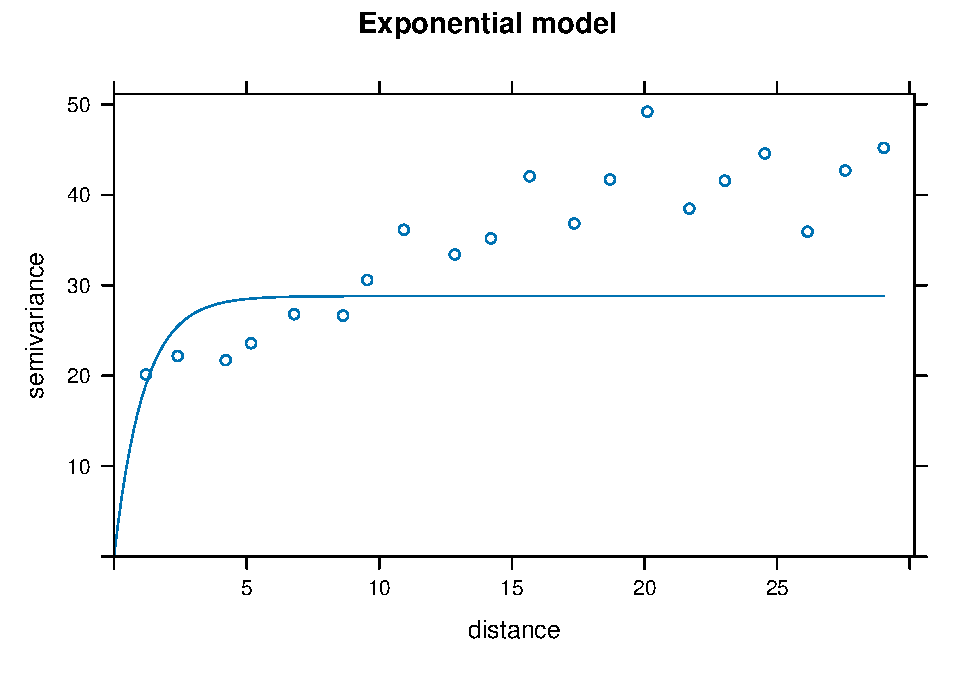
\includegraphics{Field-Trial-Spatial-Analysis-Guide_files/figure-latex/unnamed-chunk-28-1.pdf}

Hmm, that plot is not very convincing.

In this field trial, there is evidence of spatial correlation as a function of distance, but there is not evidence this spatial correlation is impacted by direction.

\textbf{Another reminder on field trends}

It's important to remember these methods are intended to describe localised spatial correlation. Field-wide spatial gradients, such as position on a slope, should be modelled as a separate trend.

\hypertarget{rcbd-r}{%
\chapter{RCBD Example: R}\label{rcbd-r}}

Here are step-by-step instructions for how to incorporate spatial covariates into analysis of a field experiment that uses a randomized complete block design. Several techniques are explored:

Load the NIN data if it is not already in your R environment:

\begin{Shaded}
\begin{Highlighting}[]
\FunctionTok{library}\NormalTok{(agridat); }\FunctionTok{library}\NormalTok{(dplyr); }\FunctionTok{library}\NormalTok{(tidyr); }\FunctionTok{library}\NormalTok{(purrr);}
\FunctionTok{library}\NormalTok{(sp)}
\end{Highlighting}
\end{Shaded}

\begin{Shaded}
\begin{Highlighting}[]
\FunctionTok{data}\NormalTok{(}\StringTok{"stroup.nin"}\NormalTok{)}

\NormalTok{Nin }\OtherTok{\textless{}{-}}\NormalTok{ stroup.nin }\SpecialCharTok{\%\textgreater{}\%} \FunctionTok{mutate}\NormalTok{(}\AttributeTok{col.width =}\NormalTok{ col }\SpecialCharTok{*} \FloatTok{1.2}\NormalTok{, }
                             \AttributeTok{row.length =}\NormalTok{ row }\SpecialCharTok{*} \FloatTok{4.3}\NormalTok{) }\SpecialCharTok{\%\textgreater{}\%} 
  \FunctionTok{fill}\NormalTok{(rep, }\AttributeTok{.direction =} \StringTok{"up"}\NormalTok{) }\SpecialCharTok{\%\textgreater{}\%}  \FunctionTok{arrange}\NormalTok{(col, row) }

\NormalTok{Nin\_na }\OtherTok{\textless{}{-}} \FunctionTok{filter}\NormalTok{(Nin, }\SpecialCharTok{!}\FunctionTok{is.na}\NormalTok{(yield))}
\NormalTok{Nin\_spatial }\OtherTok{=}\NormalTok{ Nin\_na}
\FunctionTok{coordinates}\NormalTok{(Nin\_spatial) }\OtherTok{\textless{}{-}} \ErrorTok{\textasciitilde{}}\NormalTok{ col.width }\SpecialCharTok{+}\NormalTok{ row.length}
\end{Highlighting}
\end{Shaded}

Once spatial auto-correlation has been identified in field trials, the next step is to employ a modeling technique that will reduce the impact of spatial variation on the final estimates from the analysis.

\hypertarget{prep-work}{%
\section{Prep work}\label{prep-work}}

The first thing is to run a standard linear model. A common model specification for the randomized complete block design (RCBD) is to include cultivar as a fixed effect and block as a random effect.

\begin{Shaded}
\begin{Highlighting}[]
\FunctionTok{library}\NormalTok{(nlme); }\FunctionTok{library}\NormalTok{(emmeans)}

\NormalTok{nin\_lme }\OtherTok{\textless{}{-}} \FunctionTok{lme}\NormalTok{(yield }\SpecialCharTok{\textasciitilde{}}\NormalTok{ gen, }\AttributeTok{random =} \SpecialCharTok{\textasciitilde{}}\DecValTok{1}\SpecialCharTok{|}\NormalTok{rep,}
              \AttributeTok{data =}\NormalTok{ Nin,}
              \AttributeTok{na.action =}\NormalTok{ na.exclude)}

\CommentTok{\# extract the least squares means for variety}
\NormalTok{preds\_lme }\OtherTok{\textless{}{-}} \FunctionTok{as.data.frame}\NormalTok{(}\FunctionTok{emmeans}\NormalTok{(nin\_lme, }\StringTok{"gen"}\NormalTok{))}
\end{Highlighting}
\end{Shaded}

The variables ``gen'' refers to the cultivar or breeding line being trialled, and ``rep'' is the block, and the dependent variable, ``yield'' is grain yield. Basic exploratory analysis of this data set was conducted in \ref{spatial-r}.

\hypertarget{correlated-errors}{%
\section{Correlated errors}\label{correlated-errors}}

\textbf{Gaussian Example}

In order to fit models using correlated error model, we will need to first obtain preliminary estimates of the nugget, sill and range: from fitting an empirical variogram.

\begin{Shaded}
\begin{Highlighting}[]
\FunctionTok{library}\NormalTok{(gstat)}
\NormalTok{max\_dist }\OtherTok{\textless{}{-}} \FloatTok{0.6}\SpecialCharTok{*}\FunctionTok{max}\NormalTok{(}\FunctionTok{dist}\NormalTok{(}\FunctionTok{coordinates}\NormalTok{(Nin\_spatial)))}
\NormalTok{resid.var1 }\OtherTok{\textless{}{-}}\NormalTok{ gstat}\SpecialCharTok{::}\FunctionTok{variogram}\NormalTok{(yield }\SpecialCharTok{\textasciitilde{}}\NormalTok{ rep }\SpecialCharTok{+}\NormalTok{ gen, }
                        \AttributeTok{cutoff =}\NormalTok{ max\_dist,}
                        \AttributeTok{width =}\NormalTok{ max\_dist}\SpecialCharTok{/}\DecValTok{10}\NormalTok{, }
                        \AttributeTok{data =}\NormalTok{ Nin\_spatial)}
\NormalTok{nugget\_start }\OtherTok{\textless{}{-}} \FunctionTok{min}\NormalTok{(resid.var1}\SpecialCharTok{$}\NormalTok{gamma)}
\end{Highlighting}
\end{Shaded}

In the previous section, an isotropic Gaussian function was identified as the best model for describing the decay of error correlations over distance.

\begin{Shaded}
\begin{Highlighting}[]
\NormalTok{nin\_vgm }\OtherTok{\textless{}{-}} \FunctionTok{vgm}\NormalTok{(}\AttributeTok{model =} \StringTok{"Gau"}\NormalTok{, }\AttributeTok{nugget =}\NormalTok{ nugget\_start) }
\NormalTok{nin\_variofit }\OtherTok{\textless{}{-}} \FunctionTok{fit.variogram}\NormalTok{(resid.var1, nin\_vgm)}

\NormalTok{nugget }\OtherTok{\textless{}{-}}\NormalTok{ nin\_variofit}\SpecialCharTok{$}\NormalTok{psill[}\DecValTok{1}\NormalTok{] }
\NormalTok{range }\OtherTok{\textless{}{-}}\NormalTok{ nin\_variofit}\SpecialCharTok{$}\NormalTok{range[}\DecValTok{2}\NormalTok{] }
\NormalTok{sill }\OtherTok{\textless{}{-}} \FunctionTok{sum}\NormalTok{(nin\_variofit}\SpecialCharTok{$}\NormalTok{psill) }
\NormalTok{nugget.effect }\OtherTok{\textless{}{-}}\NormalTok{  nugget}\SpecialCharTok{/}\NormalTok{sill}
\end{Highlighting}
\end{Shaded}

Create a correlated error structure using the \textbf{nlme} package.

\begin{Shaded}
\begin{Highlighting}[]
\NormalTok{cor.gaus }\OtherTok{\textless{}{-}} \FunctionTok{corSpatial}\NormalTok{(}\AttributeTok{value =} \FunctionTok{c}\NormalTok{(range, nugget.effect), }
                  \AttributeTok{form =} \SpecialCharTok{\textasciitilde{}}\NormalTok{ row.length }\SpecialCharTok{+}\NormalTok{ col.width, }
                  \AttributeTok{nugget =}\NormalTok{ T, }\AttributeTok{fixed =}\NormalTok{ F,}
                  \AttributeTok{type =} \StringTok{"gaussian"}\NormalTok{, }
                  \AttributeTok{metric =} \StringTok{"euclidean"}\NormalTok{)}
\end{Highlighting}
\end{Shaded}

Update the linear mixed model with the correlated error structure:

\begin{Shaded}
\begin{Highlighting}[]
\NormalTok{nin\_gaus }\OtherTok{\textless{}{-}} \FunctionTok{update}\NormalTok{(nin\_lme, }\AttributeTok{corr =}\NormalTok{ cor.gaus)}
\end{Highlighting}
\end{Shaded}

Extract variety estimates:

\begin{Shaded}
\begin{Highlighting}[]
\NormalTok{preds\_gaus }\OtherTok{\textless{}{-}} \FunctionTok{as.data.frame}\NormalTok{(}\FunctionTok{emmeans}\NormalTok{(nin\_gaus, }\StringTok{"gen"}\NormalTok{))}
\end{Highlighting}
\end{Shaded}

Other models can be implemented following this template.

\hypertarget{exponential-1}{%
\subsection{Exponential}\label{exponential-1}}

\begin{Shaded}
\begin{Highlighting}[]
\FunctionTok{rm}\NormalTok{(nin\_vgm, nin\_variofit, nugget, sill, range, nugget.effect)}

\NormalTok{nin\_vgm }\OtherTok{\textless{}{-}} \FunctionTok{vgm}\NormalTok{(}\AttributeTok{model =} \StringTok{"Exp"}\NormalTok{, }\AttributeTok{nugget =}\NormalTok{ nugget\_start) }
\NormalTok{nin\_variofit }\OtherTok{\textless{}{-}} \FunctionTok{fit.variogram}\NormalTok{(resid.var1, nin\_vgm)}

\NormalTok{nugget }\OtherTok{\textless{}{-}}\NormalTok{ nin\_variofit}\SpecialCharTok{$}\NormalTok{psill[}\DecValTok{1}\NormalTok{] }
\NormalTok{range }\OtherTok{\textless{}{-}}\NormalTok{ nin\_variofit}\SpecialCharTok{$}\NormalTok{range[}\DecValTok{2}\NormalTok{] }
\NormalTok{sill }\OtherTok{\textless{}{-}} \FunctionTok{sum}\NormalTok{(nin\_variofit}\SpecialCharTok{$}\NormalTok{psill) }
\NormalTok{nugget.effect }\OtherTok{\textless{}{-}}\NormalTok{  nugget}\SpecialCharTok{/}\NormalTok{sill}

\NormalTok{cor.exp }\OtherTok{\textless{}{-}} \FunctionTok{corSpatial}\NormalTok{(}\AttributeTok{value =} \FunctionTok{c}\NormalTok{(range, nugget.effect), }
                  \AttributeTok{form =} \SpecialCharTok{\textasciitilde{}}\NormalTok{ row.length }\SpecialCharTok{+}\NormalTok{ col.width, }
                  \AttributeTok{nugget =}\NormalTok{ T, }\AttributeTok{fixed =}\NormalTok{ F,}
                  \AttributeTok{type =} \StringTok{"exponential"}\NormalTok{, }
                  \AttributeTok{metric =} \StringTok{"euclidean"}\NormalTok{)}

\NormalTok{nin\_exp }\OtherTok{\textless{}{-}} \FunctionTok{update}\NormalTok{(nin\_lme, }\AttributeTok{corr =}\NormalTok{ cor.exp)}
\NormalTok{preds\_exp }\OtherTok{\textless{}{-}} \FunctionTok{as.data.frame}\NormalTok{(}\FunctionTok{emmeans}\NormalTok{(nin\_exp, }\StringTok{"gen"}\NormalTok{))}
\end{Highlighting}
\end{Shaded}

\hypertarget{spherical-1}{%
\subsection{Spherical}\label{spherical-1}}

\begin{Shaded}
\begin{Highlighting}[]
\FunctionTok{rm}\NormalTok{(nin\_vgm, nin\_variofit, nugget, sill, range, nugget.effect)}

\NormalTok{nin\_vgm }\OtherTok{\textless{}{-}} \FunctionTok{vgm}\NormalTok{(}\AttributeTok{model =} \StringTok{"Sph"}\NormalTok{, }\AttributeTok{nugget =}\NormalTok{ nugget\_start) }
\NormalTok{nin\_variofit }\OtherTok{\textless{}{-}} \FunctionTok{fit.variogram}\NormalTok{(resid.var1, nin\_vgm)}

\NormalTok{nugget }\OtherTok{\textless{}{-}}\NormalTok{ nin\_variofit}\SpecialCharTok{$}\NormalTok{psill[}\DecValTok{1}\NormalTok{] }
\NormalTok{range }\OtherTok{\textless{}{-}}\NormalTok{ nin\_variofit}\SpecialCharTok{$}\NormalTok{range[}\DecValTok{2}\NormalTok{] }
\NormalTok{sill }\OtherTok{\textless{}{-}} \FunctionTok{sum}\NormalTok{(nin\_variofit}\SpecialCharTok{$}\NormalTok{psill) }
\NormalTok{nugget.effect }\OtherTok{\textless{}{-}}\NormalTok{  nugget}\SpecialCharTok{/}\NormalTok{sill}

\NormalTok{cor.sph }\OtherTok{\textless{}{-}} \FunctionTok{corSpatial}\NormalTok{(}\AttributeTok{value =} \FunctionTok{c}\NormalTok{(range, nugget.effect), }
                  \AttributeTok{form =} \SpecialCharTok{\textasciitilde{}}\NormalTok{ row.length }\SpecialCharTok{+}\NormalTok{ col.width, }
                  \AttributeTok{nugget =}\NormalTok{ T, }\AttributeTok{fixed =}\NormalTok{ F,}
                  \AttributeTok{type =} \StringTok{"spherical"}\NormalTok{, }
                  \AttributeTok{metric =} \StringTok{"euclidean"}\NormalTok{)}

\NormalTok{nin\_sph }\OtherTok{\textless{}{-}} \FunctionTok{update}\NormalTok{(nin\_lme, }\AttributeTok{corr =}\NormalTok{ cor.sph)}
\NormalTok{preds\_sph }\OtherTok{\textless{}{-}} \FunctionTok{as.data.frame}\NormalTok{(}\FunctionTok{emmeans}\NormalTok{(nin\_sph, }\StringTok{"gen"}\NormalTok{))}
\end{Highlighting}
\end{Shaded}

\hypertarget{matuxe9rn-1}{%
\subsection{Matérn}\label{matuxe9rn-1}}

A Matérn error function is not available in \textbf{nlme}, but the package \textbf{spaMM} has written an extension implementing the Matérn, Cauchy and other covariance structures. The Matérn is demonstrated below.

\begin{Shaded}
\begin{Highlighting}[]
\FunctionTok{rm}\NormalTok{(nin\_vgm, nin\_variofit, nugget, sill, range, nugget.effect)}

\FunctionTok{library}\NormalTok{(spaMM) }\CommentTok{\# required for running \textasciigrave{}corMatern()\textasciigrave{}}

\NormalTok{nin\_vgm }\OtherTok{\textless{}{-}} \FunctionTok{vgm}\NormalTok{(}\AttributeTok{model =} \StringTok{"Mat"}\NormalTok{, }\AttributeTok{nugget =}\NormalTok{ nugget\_start) }
\NormalTok{nin\_variofit }\OtherTok{\textless{}{-}} \FunctionTok{fit.variogram}\NormalTok{(resid.var1, nin\_vgm, }\AttributeTok{fit.kappa =} \ConstantTok{TRUE}\NormalTok{)}
 
\NormalTok{nugget }\OtherTok{\textless{}{-}}\NormalTok{ nin\_variofit}\SpecialCharTok{$}\NormalTok{psill[}\DecValTok{1}\NormalTok{] }
\NormalTok{range }\OtherTok{\textless{}{-}}\NormalTok{ nin\_variofit}\SpecialCharTok{$}\NormalTok{range[}\DecValTok{2}\NormalTok{] }
\NormalTok{sill }\OtherTok{\textless{}{-}} \FunctionTok{sum}\NormalTok{(nin\_variofit}\SpecialCharTok{$}\NormalTok{psill) }
\NormalTok{nugget.effect }\OtherTok{\textless{}{-}}\NormalTok{  nugget}\SpecialCharTok{/}\NormalTok{sill}
\NormalTok{kappa }\OtherTok{\textless{}{-}}\NormalTok{ nin\_variofit}\SpecialCharTok{$}\NormalTok{kappa[}\DecValTok{2}\NormalTok{]}

\CommentTok{\# from spAMM documentation: "Warning: the range parameter used in corSpatial objects is the inverse of the scale parameter used in MaternCorr and thus they have opposite meaning despite both being denoted ρ elsewhere in this package or in nlme literature" {-} so range is expressed as an inverse}
\NormalTok{cor.mat }\OtherTok{\textless{}{-}} \FunctionTok{corMatern}\NormalTok{(}\AttributeTok{value =} \FunctionTok{c}\NormalTok{(}\DecValTok{1}\SpecialCharTok{/}\NormalTok{range, kappa, nugget.effect), }
                  \AttributeTok{form =} \SpecialCharTok{\textasciitilde{}}\NormalTok{ row.length }\SpecialCharTok{+}\NormalTok{ col.width, }
                  \AttributeTok{nugget =}\NormalTok{ T, }\AttributeTok{fixed =}\NormalTok{ F,}
                  \AttributeTok{metric =} \StringTok{"euclidean"}\NormalTok{)}
\NormalTok{nin\_matern }\OtherTok{\textless{}{-}} \FunctionTok{update}\NormalTok{(nin\_lme, }\AttributeTok{corr =}\NormalTok{ cor.mat)}

\NormalTok{preds\_mat }\OtherTok{\textless{}{-}} \FunctionTok{as.data.frame}\NormalTok{(}\FunctionTok{emmeans}\NormalTok{(nin\_matern, }\StringTok{"gen"}\NormalTok{))}
\end{Highlighting}
\end{Shaded}

In the \textbf{nlme} package, there is also an option for a linear model in the \texttt{corSpatial()} function. However, if a linear trend is present without a range or sill, it is recommended that a linear trend be fitted to the data instead.

\hypertarget{rowcolumn-trends}{%
\section{Row/Column Trends:}\label{rowcolumn-trends}}

The package \textbf{lme4} is used since it can handle multiple random effects while \textbf{nlme} cannot do this without nesting the effects. I prefer \textbf{nlme} for linear modeling in this tutorial because of its built-in functionality for including spatial variation.

\begin{Shaded}
\begin{Highlighting}[]
\FunctionTok{library}\NormalTok{(lme4); }\FunctionTok{library}\NormalTok{(lmerTest)}
\end{Highlighting}
\end{Shaded}

\begin{Shaded}
\begin{Highlighting}[]
\CommentTok{\# variables specifying row and column as factors are needed}
\NormalTok{Nin}\SpecialCharTok{$}\NormalTok{colF }\OtherTok{\textless{}{-}} \FunctionTok{as.factor}\NormalTok{(Nin}\SpecialCharTok{$}\NormalTok{col)}
\NormalTok{Nin}\SpecialCharTok{$}\NormalTok{rowF }\OtherTok{\textless{}{-}} \FunctionTok{as.factor}\NormalTok{(Nin}\SpecialCharTok{$}\NormalTok{row)}

\NormalTok{nin\_trend }\OtherTok{\textless{}{-}} \FunctionTok{lmer}\NormalTok{(yield }\SpecialCharTok{\textasciitilde{}}\NormalTok{ gen }\SpecialCharTok{+}\NormalTok{ (}\DecValTok{1}\SpecialCharTok{|}\NormalTok{rep) }\SpecialCharTok{+}\NormalTok{ (}\DecValTok{1}\SpecialCharTok{|}\NormalTok{colF) }\SpecialCharTok{+}\NormalTok{ (}\DecValTok{1}\SpecialCharTok{|}\NormalTok{rowF),}
              \AttributeTok{data =}\NormalTok{ Nin,}
              \AttributeTok{na.action =}\NormalTok{ na.exclude)}

\NormalTok{preds\_trend }\OtherTok{\textless{}{-}} \FunctionTok{as.data.frame}\NormalTok{(}\FunctionTok{emmeans}\NormalTok{(nin\_trend, }\StringTok{"gen"}\NormalTok{))}
\end{Highlighting}
\end{Shaded}

\begin{verbatim}
## Cannot use mode = "kenward-roger" because *pbkrtest* package is not installed
\end{verbatim}

\hypertarget{splines-1}{%
\section{Splines}\label{splines-1}}

The package \textbf{SpATS}, ``spatial analysis for field trials'', implements B-splines for row and column effects.

\begin{Shaded}
\begin{Highlighting}[]
\FunctionTok{library}\NormalTok{(SpATS)}

\NormalTok{nin\_spline }\OtherTok{\textless{}{-}} \FunctionTok{SpATS}\NormalTok{(}\AttributeTok{response =} \StringTok{"yield"}\NormalTok{, }
                    \AttributeTok{spatial =} \SpecialCharTok{\textasciitilde{}} \FunctionTok{PSANOVA}\NormalTok{(col, row, }\AttributeTok{nseg =} \FunctionTok{c}\NormalTok{(}\DecValTok{10}\NormalTok{,}\DecValTok{20}\NormalTok{),}
                                        \AttributeTok{degree =} \DecValTok{3}\NormalTok{, }\AttributeTok{pord =} \DecValTok{2}\NormalTok{), }
                    \AttributeTok{genotype =} \StringTok{"gen"}\NormalTok{,  }
                    \AttributeTok{random =} \SpecialCharTok{\textasciitilde{}}\NormalTok{ rep, }\CommentTok{\# + rowF + colF, }
                    \AttributeTok{data =}\NormalTok{ Nin, }
                    \AttributeTok{control =} \FunctionTok{list}\NormalTok{(}\AttributeTok{tolerance =} \FloatTok{1e{-}03}\NormalTok{, }\AttributeTok{monitoring =} \DecValTok{0}\NormalTok{))}

\NormalTok{preds\_spline }\OtherTok{\textless{}{-}} \FunctionTok{predict}\NormalTok{(nin\_spline, }\AttributeTok{which =} \StringTok{"gen"}\NormalTok{) }\SpecialCharTok{\%\textgreater{}\%} 
\NormalTok{  dplyr}\SpecialCharTok{::}\FunctionTok{select}\NormalTok{(gen, }\AttributeTok{emmean =} \StringTok{"predicted.values"}\NormalTok{, }\AttributeTok{SE =} \StringTok{"standard.errors"}\NormalTok{)}
\end{Highlighting}
\end{Shaded}

\hypertarget{ar1xar1}{%
\section{AR1xAR1}\label{ar1xar1}}

The estimates for \(\rho\) are determined via a grid search. The default grid searches the entire space, ({[}-1, 1{]} for rows and columns) We can narrow down the grid search to the area most impactful based on log likelihood.

\begin{Shaded}
\begin{Highlighting}[]
\FunctionTok{qplot}\NormalTok{(rho\_r, rho\_c, }\AttributeTok{fill =}\NormalTok{ loglik, }\AttributeTok{geom =} \StringTok{\textquotesingle{}tile\textquotesingle{}}\NormalTok{, }\AttributeTok{data =}\NormalTok{ nin\_ar1ar1}\SpecialCharTok{$}\NormalTok{rho)}
\end{Highlighting}
\end{Shaded}

\begin{verbatim}
## Warning: `qplot()` was deprecated in ggplot2 3.4.0.
## This warning is displayed once every 8 hours.
## Call `lifecycle::last_lifecycle_warnings()` to see where this warning was
## generated.
\end{verbatim}

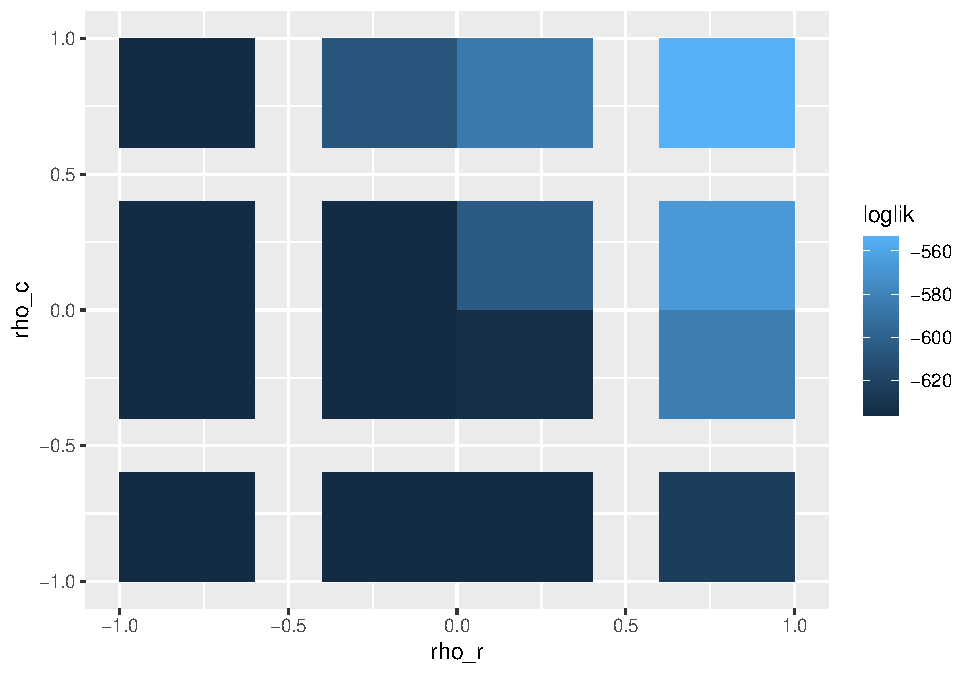
\includegraphics{Field-Trial-Spatial-Analysis-Guide_files/figure-latex/unnamed-chunk-44-1.pdf}

\begin{Shaded}
\begin{Highlighting}[]
\CommentTok{\# Refine the grid around the most likely values (the range cannot contain exactly 1 or {-}1)}
\NormalTok{rho.grid }\OtherTok{\textless{}{-}} \FunctionTok{expand.grid}\NormalTok{(}\AttributeTok{rho\_r =} \FunctionTok{seq}\NormalTok{(}\FloatTok{0.5}\NormalTok{, }\FloatTok{0.95}\NormalTok{, }\AttributeTok{length =} \DecValTok{4}\NormalTok{),}
                        \AttributeTok{rho\_c =} \FunctionTok{seq}\NormalTok{(}\FloatTok{0.5}\NormalTok{, }\FloatTok{0.95}\NormalTok{, }\AttributeTok{length =} \DecValTok{4}\NormalTok{))}
\end{Highlighting}
\end{Shaded}

\hypertarget{bayesian-ar1xar1}{%
\section{Bayesian AR1xAR1}\label{bayesian-ar1xar1}}

\begin{Shaded}
\begin{Highlighting}[]
\CommentTok{\#library(INLA) }
\DocumentationTok{\#\# under construction....}
\end{Highlighting}
\end{Shaded}

\hypertarget{model-selection}{%
\section{Model Selection}\label{model-selection}}

Now that we have built these spatial models, how do we pick the right one? Unfortunately, there is no one model that works best in all circumstances. In addition, there is no single way for choosing the best model! Some approaches include:

\begin{enumerate}
\def\labelenumi{\arabic{enumi}.}
\tightlist
\item
  comparing model fitness (e.g.~AIC, BIC, log likelihood)
\item
  comparing post-hoc power (that is, the p-values for the treatments)
\item
  comparing standard error of the estimates
\end{enumerate}

In order to make comparisons, the code below assembles all the model objects into one list. They are generated from different processes, as shown by the \texttt{class} attribute of each one, so this takes some data conditioning.

\begin{Shaded}
\begin{Highlighting}[]
\NormalTok{all.models }\OtherTok{\textless{}{-}} \FunctionTok{mget}\NormalTok{(}\FunctionTok{ls}\NormalTok{(}\AttributeTok{pattern =} \StringTok{"\^{}nin\_*"}\NormalTok{))}
\CommentTok{\# print out their class}
\FunctionTok{map}\NormalTok{(all.models, class)}
\end{Highlighting}
\end{Shaded}

\begin{verbatim}
## $nin.lme
## [1] "lme"
## 
## $nin_ar1ar1
## [1] "breedR"  "remlf90"
## 
## $nin_exp
## [1] "lme"
## 
## $nin_gaus
## [1] "lme"
## 
## $nin_lme
## [1] "lme"
## 
## $nin_matern
## [1] "lme"
## 
## $nin_sph
## [1] "lme"
## 
## $nin_spline
## [1] "SpATS"
## 
## $nin_trend
## [1] "lmerModLmerTest"
## attr(,"package")
## [1] "lmerTest"
\end{verbatim}

\hypertarget{spatial-dependence-of-residuals}{%
\subsection{Spatial dependence of residuals}\label{spatial-dependence-of-residuals}}

It would be helpful to know if these methods were effective in reducing the spatial autocorrelation among the error residuals.

The function below extracts the residuals from each model and is needed because of different handling of missing values by the package \textbf{SpATS}.

\begin{Shaded}
\begin{Highlighting}[]
\NormalTok{L1 }\OtherTok{\textless{}{-}} \FunctionTok{nrow}\NormalTok{(Nin)}
\NormalTok{non\_na }\OtherTok{\textless{}{-}} \SpecialCharTok{!}\FunctionTok{is.na}\NormalTok{(Nin}\SpecialCharTok{$}\NormalTok{yield)}
\NormalTok{L2 }\OtherTok{\textless{}{-}} \FunctionTok{sum}\NormalTok{(non\_na)}

\NormalTok{residuals }\OtherTok{\textless{}{-}} \FunctionTok{map}\NormalTok{(all.models, }\ControlFlowTok{function}\NormalTok{ (x) \{}
  
\NormalTok{  resids }\OtherTok{\textless{}{-}} \FunctionTok{residuals}\NormalTok{(x)}
  
  \ControlFlowTok{if}\NormalTok{(}\FunctionTok{is.data.frame}\NormalTok{(resids)) \{}
\NormalTok{    colnum }\OtherTok{=} \FunctionTok{ncol}\NormalTok{(resids)}
\NormalTok{    resids }\OtherTok{=}\NormalTok{ resids[,colnum]}
\NormalTok{  \}}
  
  \ControlFlowTok{if}\NormalTok{(}\FunctionTok{length}\NormalTok{(resids) }\SpecialCharTok{==}\NormalTok{ L2) \{}
\NormalTok{    resids\_pl }\OtherTok{=} \FunctionTok{rep}\NormalTok{(}\ConstantTok{NA}\NormalTok{, L1)}
\NormalTok{    resids\_pl[non\_na] }\OtherTok{=}\NormalTok{ resids}
\NormalTok{    resids }\OtherTok{=}\NormalTok{ resids\_pl}
\NormalTok{  \}}
  \FunctionTok{return}\NormalTok{(resids)}
\NormalTok{\})}

\FunctionTok{names}\NormalTok{(residuals) }\OtherTok{\textless{}{-}} \FunctionTok{names}\NormalTok{(all.models)}
\end{Highlighting}
\end{Shaded}

Run a Moran's I test on the extracted residuals:

\begin{Shaded}
\begin{Highlighting}[]
\FunctionTok{library}\NormalTok{(spdep)}

\NormalTok{xy.rook }\OtherTok{\textless{}{-}} \FunctionTok{cell2nb}\NormalTok{(}\AttributeTok{nrow =} \FunctionTok{max}\NormalTok{(Nin}\SpecialCharTok{$}\NormalTok{row), }\AttributeTok{ncol =} \FunctionTok{max}\NormalTok{(Nin}\SpecialCharTok{$}\NormalTok{col), }\AttributeTok{type=}\StringTok{"rook"}\NormalTok{)}

\NormalTok{Moran.I }\OtherTok{\textless{}{-}} \FunctionTok{map\_df}\NormalTok{(residuals, }\ControlFlowTok{function}\NormalTok{(x) \{}
\NormalTok{  mi }\OtherTok{=} \FunctionTok{moran.test}\NormalTok{(x, }\FunctionTok{nb2listw}\NormalTok{(xy.rook), }\AttributeTok{na.action =}\NormalTok{ na.exclude)}
\NormalTok{  mi.stat }\OtherTok{\textless{}{-}}\NormalTok{ mi}\SpecialCharTok{$}\NormalTok{estimate}
\NormalTok{  mi.stat}\SpecialCharTok{$}\NormalTok{p.value }\OtherTok{\textless{}{-}}\NormalTok{ mi}\SpecialCharTok{$}\NormalTok{p.value}
  \FunctionTok{return}\NormalTok{(mi.stat)}
\NormalTok{\}) }\SpecialCharTok{\%\textgreater{}\%} \FunctionTok{mutate}\NormalTok{(}\AttributeTok{model =} \FunctionTok{names}\NormalTok{(all.models)) }\SpecialCharTok{\%\textgreater{}\%}\NormalTok{ dplyr}\SpecialCharTok{::}\FunctionTok{select}\NormalTok{(}\FunctionTok{c}\NormalTok{(}\DecValTok{5}\NormalTok{, }\DecValTok{1}\SpecialCharTok{:}\DecValTok{4}\NormalTok{)) }\SpecialCharTok{\%\textgreater{}\%} 
  \FunctionTok{mutate\_at}\NormalTok{(}\DecValTok{2}\SpecialCharTok{:}\DecValTok{5}\NormalTok{, round, }\DecValTok{4}\NormalTok{) }\SpecialCharTok{\%\textgreater{}\%} \FunctionTok{arrange}\NormalTok{(p.value)}

\NormalTok{Moran.I}
\end{Highlighting}
\end{Shaded}

\begin{verbatim}
## # A tibble: 9 x 5
##   model      `Moran I statistic` Expectation Variance p.value
##   <chr>                    <dbl>       <dbl>    <dbl>   <dbl>
## 1 nin.lme                 0.402      -0.0045   0.0025  0     
## 2 nin_exp                 0.756      -0.0045   0.0025  0     
## 3 nin_gaus                0.760      -0.0045   0.0025  0     
## 4 nin_lme                 0.402      -0.0045   0.0025  0     
## 5 nin_matern              0.760      -0.0045   0.0025  0     
## 6 nin_sph                 0.757      -0.0045   0.0025  0     
## 7 nin_trend               0.132      -0.0045   0.0025  0.0032
## 8 nin_spline             -0.0514     -0.0045   0.0025  0.826 
## 9 nin_ar1ar1             -0.112      -0.0045   0.0025  0.984
\end{verbatim}

Only one model, \texttt{nin\_spline} resulted in an improvement in Moran's I. Nearest neighbor approaches can also improve Moran's I. The significant p-values indicate that auto-correlation is still present in those models. However, that doesn't mean the other models are ineffective. The other models incorporate the spatial auto-correlation directly into the error terms.

\hypertarget{compare-model-fit}{%
\subsection{Compare Model Fit}\label{compare-model-fit}}

\emph{log likelihood, AIC, BIC}

Since these are not nested models, likelihood ratio tests cannot be performed. Log likelihood can be compared within the models from \textbf{nlme} but not across packages since they use different estimation procedures.

\begin{Shaded}
\begin{Highlighting}[]
\NormalTok{nlme\_mods }\OtherTok{\textless{}{-}} \FunctionTok{list}\NormalTok{(nin\_lme, nin\_trend, nin\_exp, nin\_gaus, nin\_sph, nin\_matern, nin\_ar1ar1)}

\FunctionTok{names}\NormalTok{(nlme\_mods) }\OtherTok{\textless{}{-}} \FunctionTok{c}\NormalTok{(}\StringTok{"LMM"}\NormalTok{, }\StringTok{"row{-}col\_trend"}\NormalTok{, }\StringTok{"exponential"}\NormalTok{, }
                        \StringTok{"gaussian"}\NormalTok{, }\StringTok{"spherical"}\NormalTok{, }\StringTok{"matern"}\NormalTok{, }\StringTok{"AR1xAR1"}\NormalTok{)}

\FunctionTok{data.frame}\NormalTok{(}\AttributeTok{logLiklihood =} \FunctionTok{sapply}\NormalTok{(nlme\_mods, logLik),}
           \AttributeTok{AIC =} \FunctionTok{sapply}\NormalTok{(nlme\_mods, AIC),}
           \AttributeTok{BIC =} \FunctionTok{sapply}\NormalTok{(nlme\_mods, AIC, }\AttributeTok{k =} \FunctionTok{log}\NormalTok{(}\FunctionTok{nrow}\NormalTok{(Nin\_na)))) }\SpecialCharTok{\%\textgreater{}\%} \FunctionTok{arrange}\NormalTok{(}\FunctionTok{desc}\NormalTok{(logLiklihood))}
\end{Highlighting}
\end{Shaded}

\begin{verbatim}
##               logLiklihood      AIC      BIC
## matern           -540.3386 1202.677 1410.788
## gaussian         -540.3401 1200.680 1405.379
## spherical        -541.7560 1203.512 1408.211
## exponential      -543.0149 1206.030 1410.729
## AR1xAR1          -550.4486 1104.897 1111.721
## row-col_trend    -577.6523 1275.305 1480.003
## LMM              -608.8508 1333.702 1531.577
\end{verbatim}

Larger log likelihoods indicate a better fitting model to the data. A rule of thumb when comparing log likelihoods is that differences less than 2 are not considered notable. These results suggest that the Gaussian, spherical, power and Matérn models are substantially equivalent in capturing the variation present in this data set.

\hypertarget{experiment-wide-error}{%
\subsection{Experiment-wide error}\label{experiment-wide-error}}

\begin{Shaded}
\begin{Highlighting}[]
\NormalTok{exp\_error }\OtherTok{\textless{}{-}} \FunctionTok{as.data.frame}\NormalTok{(}\FunctionTok{sapply}\NormalTok{(nlme\_mods[}\SpecialCharTok{{-}}\DecValTok{7}\NormalTok{], sigma))}
\NormalTok{exp\_error}
\end{Highlighting}
\end{Shaded}

\begin{verbatim}
##               sapply(nlme_mods[-7], sigma)
## LMM                               7.041475
## row-col_trend                     4.754971
## exponential                       8.967355
## gaussian                          8.035251
## spherical                         7.946038
## matern                            8.061689
\end{verbatim}

The overall experimental error, \(\sigma\), increased slightly in the correlated error models because field variation has been re-partitioned to the error when it was (erroneously) absorbed by the other experimental effects.

As a result, the coefficient of variation is not a good metric for evaluating the quality of spatial models.

\begin{Shaded}
\begin{Highlighting}[]
\NormalTok{CV }\OtherTok{=} \FunctionTok{sapply}\NormalTok{(nlme\_mods[}\SpecialCharTok{{-}}\DecValTok{7}\NormalTok{], }\ControlFlowTok{function}\NormalTok{(x) \{}
  \FunctionTok{sigma}\NormalTok{(x)}\SpecialCharTok{/}\FunctionTok{mean}\NormalTok{(}\FunctionTok{fitted}\NormalTok{(x), }\AttributeTok{na.rm =}\NormalTok{ T) }\SpecialCharTok{*} \DecValTok{100}
\NormalTok{\})}
\FunctionTok{as.data.frame}\NormalTok{(CV)}
\end{Highlighting}
\end{Shaded}

\begin{verbatim}
##                     CV
## LMM           27.58441
## row-col_trend 18.62722
## exponential   35.99247
## gaussian      30.68459
## spherical     31.74386
## matern        30.81737
\end{verbatim}

\hypertarget{post-hoc-power}{%
\subsection{Post-hoc power}\label{post-hoc-power}}

Simulation studies indicate that incorporating spatial correlation into field trial analysis can improve the overall power of the experiment (the probability of detecting true differences in treatments). When working with data from a completed experiment, power is a transformed p-value. Performing ANOVA can indicate which approach maximizes power.

\begin{Shaded}
\begin{Highlighting}[]
\NormalTok{anovas }\OtherTok{\textless{}{-}} \FunctionTok{lapply}\NormalTok{(nlme\_mods[}\SpecialCharTok{{-}}\DecValTok{7}\NormalTok{], }\ControlFlowTok{function}\NormalTok{(x)\{ }
\NormalTok{  aov }\OtherTok{\textless{}{-}} \FunctionTok{as.data.frame}\NormalTok{(}\FunctionTok{anova}\NormalTok{(x))[}\DecValTok{2}\NormalTok{,]}
\NormalTok{  \})}

\NormalTok{a }\OtherTok{\textless{}{-}} \FunctionTok{bind\_rows}\NormalTok{(anovas) }\SpecialCharTok{\%\textgreater{}\%} \FunctionTok{mutate}\NormalTok{(}\AttributeTok{model =} \FunctionTok{c}\NormalTok{(}\StringTok{"LMM"}\NormalTok{, }\StringTok{"row/column trend"}\NormalTok{, }\StringTok{"exponential"}\NormalTok{, }
                                       \StringTok{"gaussian"}\NormalTok{, }\StringTok{"spherical"}\NormalTok{, }\StringTok{"matern"}\NormalTok{)) }\SpecialCharTok{\%\textgreater{}\%} 
  \FunctionTok{arrange}\NormalTok{(}\FunctionTok{desc}\NormalTok{(}\StringTok{\textasciigrave{}}\AttributeTok{p{-}value}\StringTok{\textasciigrave{}}\NormalTok{)) }\SpecialCharTok{\%\textgreater{}\%}\NormalTok{ dplyr}\SpecialCharTok{::}\FunctionTok{select}\NormalTok{(}\FunctionTok{c}\NormalTok{(model, }\DecValTok{1}\SpecialCharTok{:}\DecValTok{4}\NormalTok{)) }\SpecialCharTok{\%\textgreater{}\%}\NormalTok{ tibble}\SpecialCharTok{::}\FunctionTok{remove\_rownames}\NormalTok{() }

\NormalTok{a[}\DecValTok{6}\NormalTok{,}\DecValTok{2}\SpecialCharTok{:}\DecValTok{5}\NormalTok{] }\OtherTok{\textless{}{-}} \FunctionTok{anova}\NormalTok{(nin\_trend)[}\DecValTok{3}\SpecialCharTok{:}\DecValTok{6}\NormalTok{]}
\NormalTok{a}
\end{Highlighting}
\end{Shaded}

\begin{verbatim}
##              model numDF    denDF   F-value     p-value
## 1              LMM    55 165.0000 0.8754898 0.711852150
## 2         gaussian    55 165.0000 1.7815059 0.002816775
## 3           matern    55 165.0000 1.7816169 0.002814130
## 4      exponential    55 165.0000 1.8348864 0.001786539
## 5        spherical    55 165.0000 1.8370929 0.001752953
## 6 row/column trend    55 132.3739 1.3101069 0.107626854
\end{verbatim}

This table indicates changes in the hypothesis test for ``gen''. There is a dramatic change in power for this test when incorporating spatial covariance structures.

\hypertarget{standard-error-of-treatment-means}{%
\subsection{Standard error of treatment means}\label{standard-error-of-treatment-means}}

Retrieve predictions generated in the previous section:

\begin{Shaded}
\begin{Highlighting}[]
\CommentTok{\#(standardise names for downstream merging step)}
\CommentTok{\#preds\_ar1ar1 \textless{}{-} preds\_ar1ar1  \%\textgreater{}\% rename(emmean = "predicted.value", SE = "standard.error") }
\NormalTok{all.preds }\OtherTok{\textless{}{-}} \FunctionTok{mget}\NormalTok{(}\FunctionTok{ls}\NormalTok{(}\AttributeTok{pattern =} \StringTok{"\^{}preds\_*"}\NormalTok{)) }
\end{Highlighting}
\end{Shaded}

Extract standard errors and plot:

\begin{Shaded}
\begin{Highlighting}[]
\NormalTok{errors }\OtherTok{\textless{}{-}} \FunctionTok{lapply}\NormalTok{(all.preds, }\StringTok{"["}\NormalTok{, }\StringTok{"SE"}\NormalTok{)}
\NormalTok{pred.names }\OtherTok{\textless{}{-}} \FunctionTok{gsub}\NormalTok{(}\StringTok{"preds\_"}\NormalTok{, }\StringTok{""}\NormalTok{, }\FunctionTok{names}\NormalTok{(errors))}
\NormalTok{error\_df }\OtherTok{\textless{}{-}} \FunctionTok{bind\_cols}\NormalTok{(errors)}
\FunctionTok{colnames}\NormalTok{(error\_df) }\OtherTok{\textless{}{-}}\NormalTok{ pred.names}
\end{Highlighting}
\end{Shaded}

\begin{figure}

{\centering 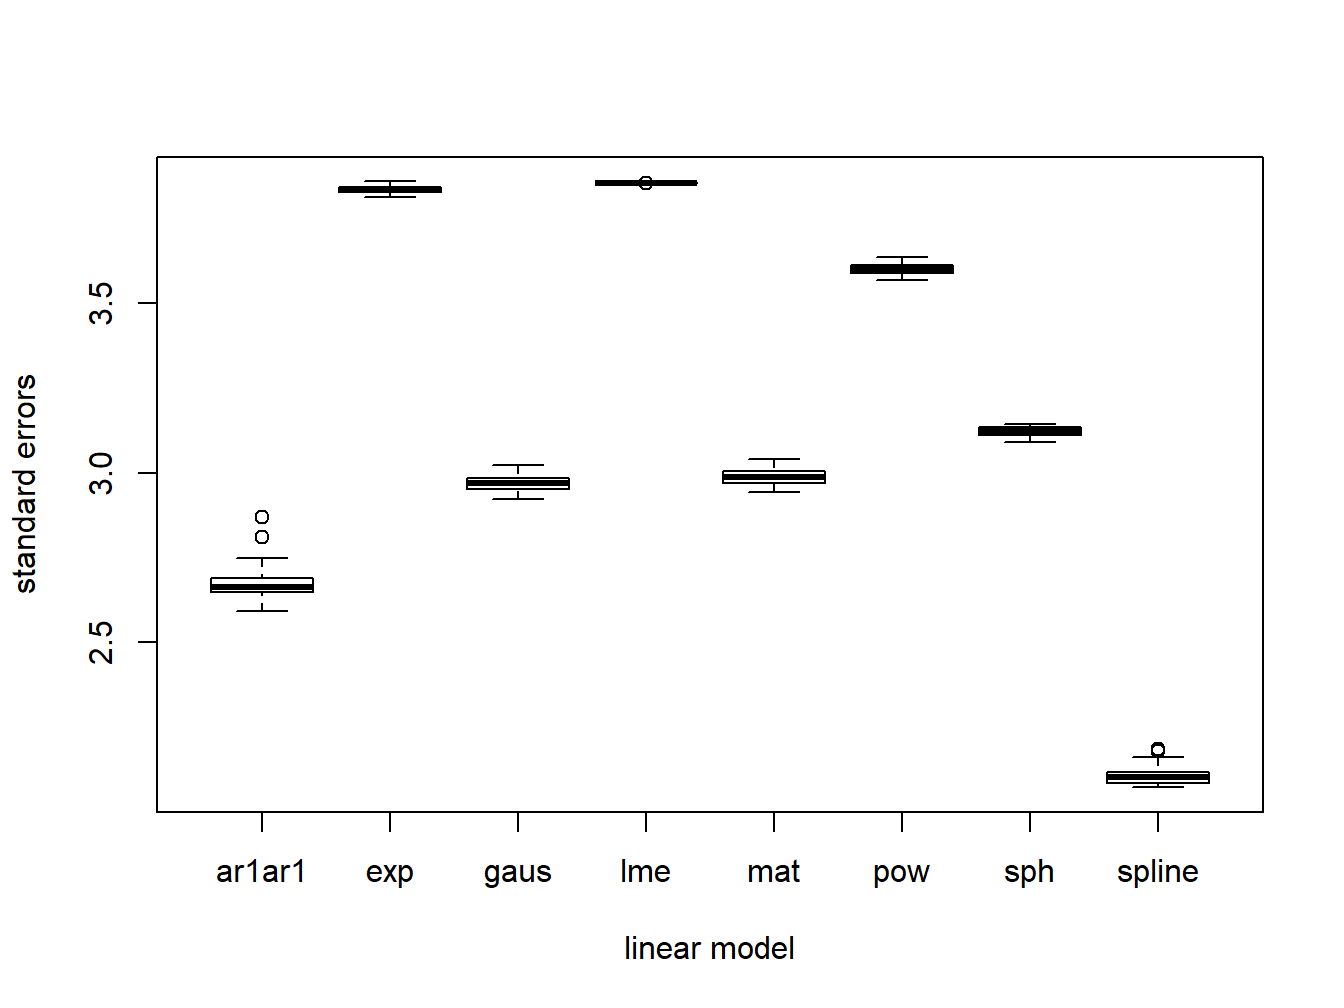
\includegraphics[width=0.8\linewidth]{Field-Trial-Spatial-Analysis-Guide_files/figure-latex/SE-box-fig-1} 

}

\caption{Differences in Variety Standard Error}\label{fig:SE-box-fig}
\end{figure}

\hypertarget{treatment-means}{%
\subsection{Treatment means}\label{treatment-means}}

Extract estimates:

\begin{Shaded}
\begin{Highlighting}[]
\NormalTok{preds }\OtherTok{\textless{}{-}} \FunctionTok{lapply}\NormalTok{(all.preds, }\StringTok{"["}\NormalTok{, }\StringTok{"emmean"}\NormalTok{)}
\NormalTok{preds\_df }\OtherTok{\textless{}{-}} \FunctionTok{bind\_cols}\NormalTok{(preds)}
\FunctionTok{colnames}\NormalTok{(preds\_df) }\OtherTok{\textless{}{-}}\NormalTok{ pred.names}
\NormalTok{preds\_df}\SpecialCharTok{$}\NormalTok{gen }\OtherTok{\textless{}{-}}\NormalTok{ preds\_exp}\SpecialCharTok{$}\NormalTok{gen}
\end{Highlighting}
\end{Shaded}

Plot changes in ranks:

\begin{figure}

{\centering 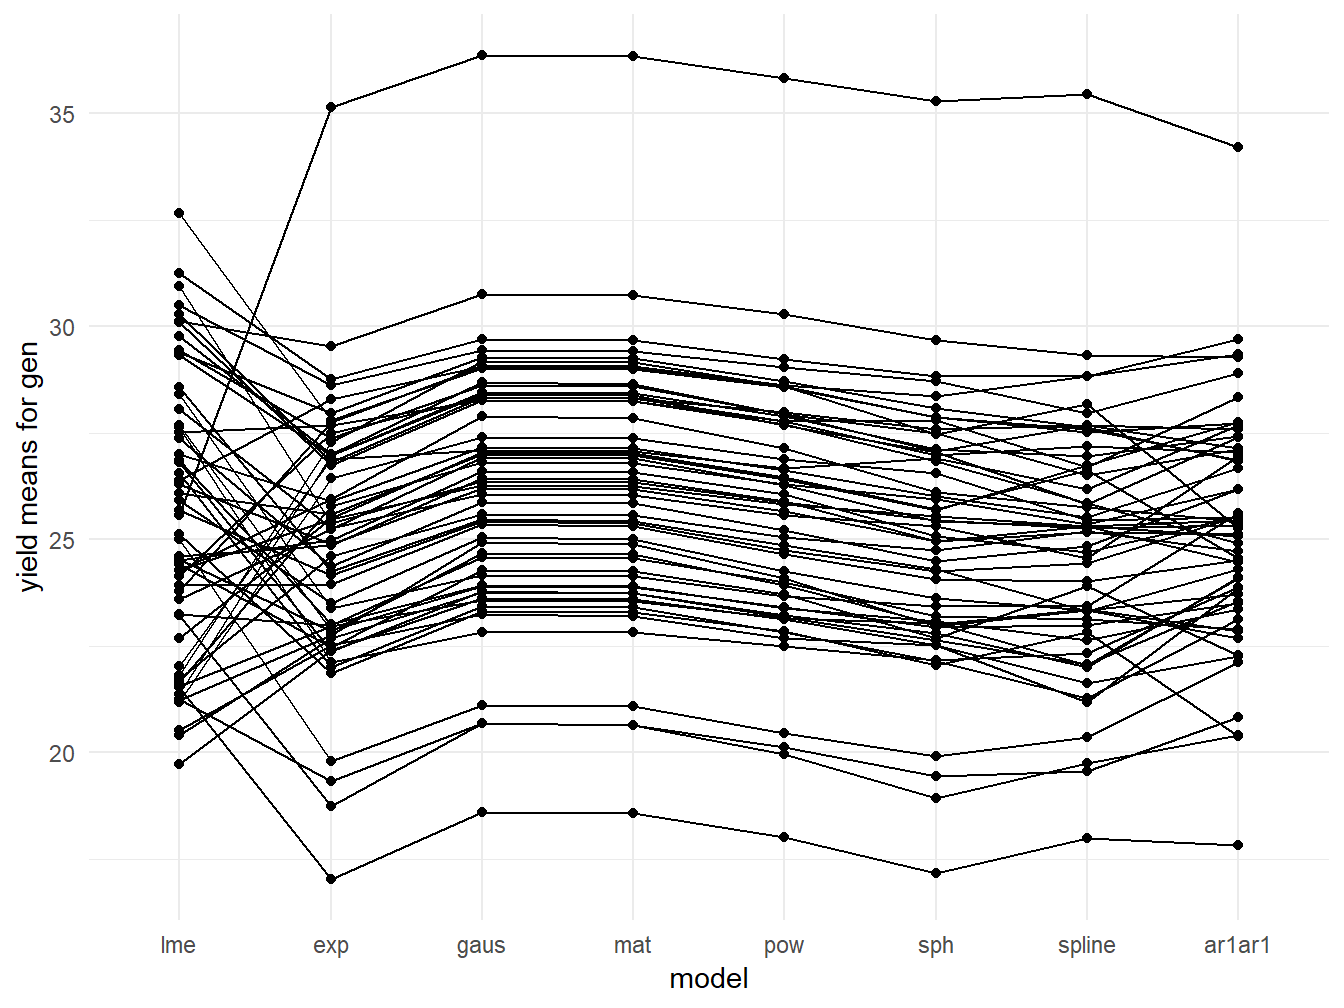
\includegraphics[width=0.85\linewidth]{Field-Trial-Spatial-Analysis-Guide_files/figure-latex/gen-ranks-fig-1} 

}

\caption{Differences in Variety Ranks}\label{fig:gen-ranks-fig}
\end{figure}

The black lines link the least squares means for a single variety. There is some consistency in the rankings between exponential, Gaussian, Matérn, and spherical covariance models. The control RCBD model, ``lme'', has fundamentally different rankings. The spline and AR1xAR1 ranking are also sightly different from the other models.

Nevertheless, the following plot indicates considerable consensus in the least squares means from all of the spatial models. The upper diagonal contains Pearson correlations between those values.

\begin{figure}

{\centering 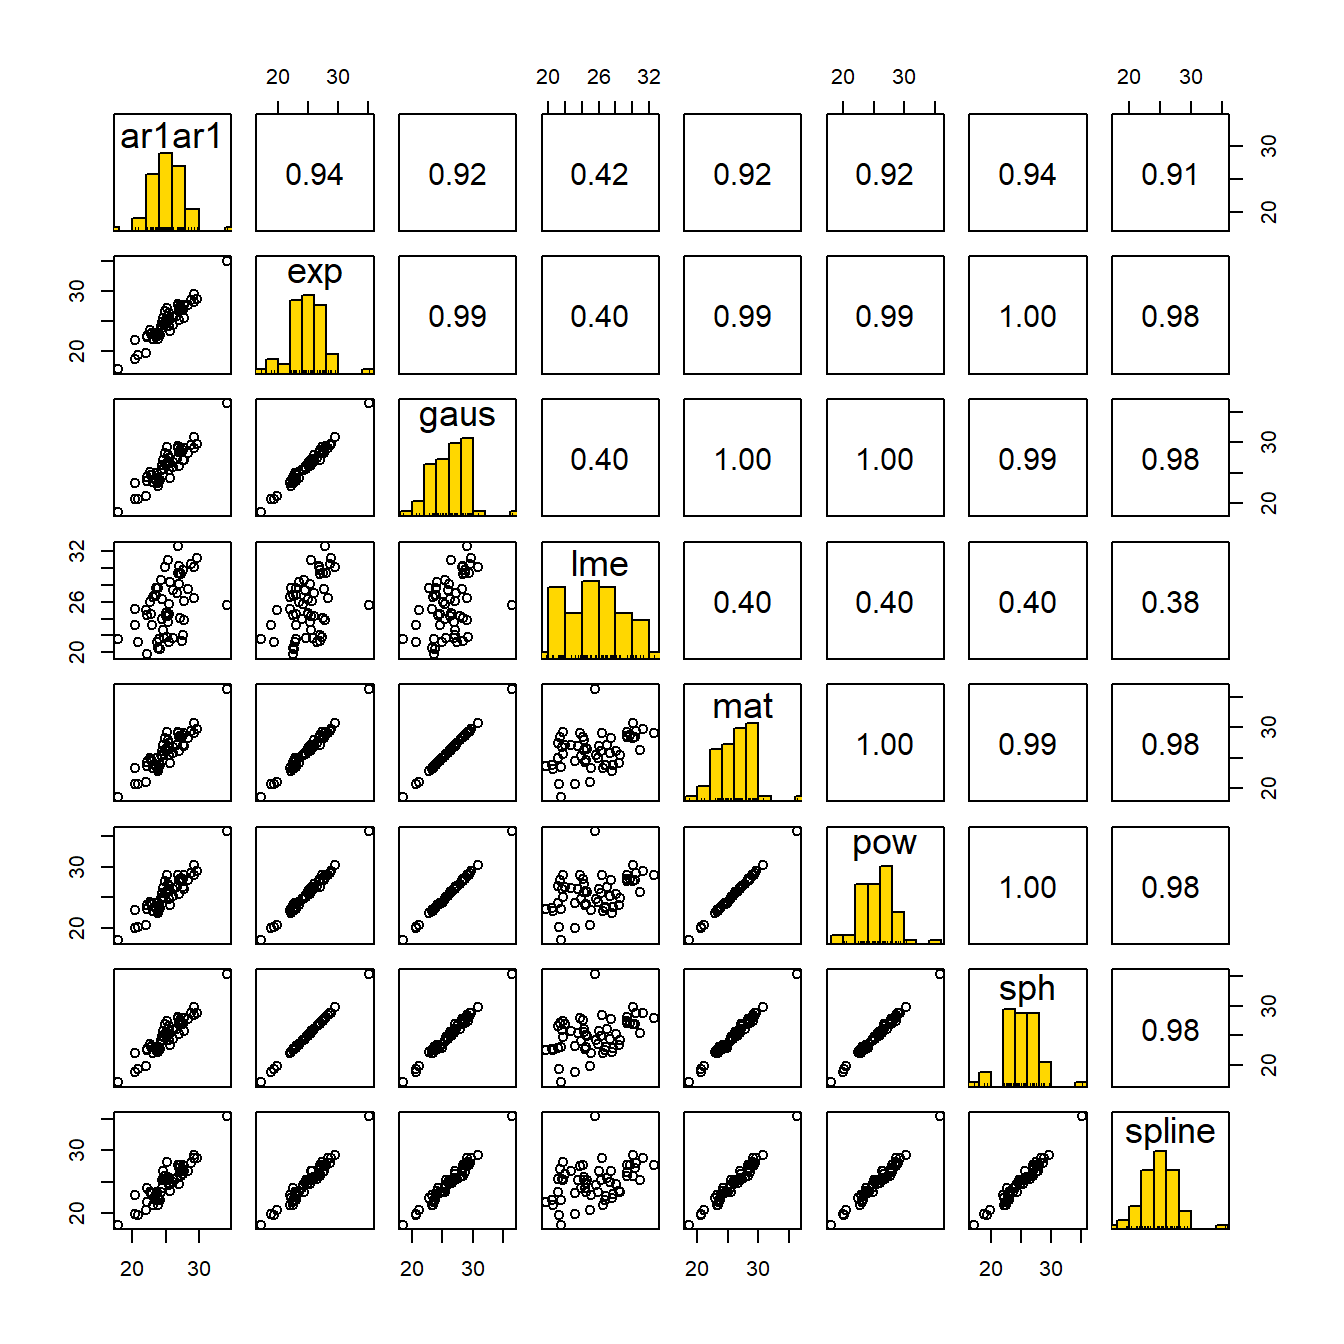
\includegraphics[width=0.9\linewidth]{Field-Trial-Spatial-Analysis-Guide_files/figure-latex/ls-panel-fig-1} 

}

\caption{Correlations in Variety Means}\label{fig:ls-panel-fig}
\end{figure}

\hypertarget{making-decisions}{%
\section{Making decisions}\label{making-decisions}}

There is no consensus on how to pick the best model. Some studies rely on log likelihood, while others seek to maximize the experimental power. Others have sought to minimize the root mean square error from cross validation.

The evidence suggest that for this data set, using any spatial model is better than running a naïve RCBD model.

\hypertarget{rcbd-sas}{%
\chapter{RCBD Example: SAS}\label{rcbd-sas}}

\hypertarget{load-and-explore-data}{%
\section{Load and Explore Data}\label{load-and-explore-data}}

These data are from a winter wheat variety trial in Alliance, Nebraska \citep{stroup1994} and are commonly used to demonstrate spatial adjustment in linear modeling. The data represent yields of 56 varieties originally laid out in a randomized complete block design (RCB). The local topography combined with winter kill, however, induced spatial variability that did not correspond to the RCB design \citep{stroup2013} which produced biased estimates in a standard unadjusted analysis.

The code below reads the data from a CSV file located the GitHub repo for this book. The data file can be downloaded from \href{https://raw.githubusercontent.com/IdahoAgStats/guide-to-field-trial-spatial-analysis/master/data/stroup_nin_wheat.csv}{here}. In this file, missing values for yield are denoted as `NA'. These values are not actually missing, but represent blank plots separating blocks in the original design of the study. The \textbf{PROC FORMAT} section converts these to numeric missing values in SAS (defined as a single period). They are then removed from the data before proceeding to analyses. Also note that row and column indices are multiplied by constants to convert them to the meter dimensions of the plots. .

The first six observations are displayed. The data contains variables for variety (gen), replication (rep), yield, and column and row identifiers. Last, a map of the 4 replications (blocks) from the original experimental design is shown.

\begin{Shaded}
\begin{Highlighting}[]
\NormalTok{proc format;}
\NormalTok{  invalue has\_NA}
\NormalTok{  \textquotesingle{}NA\textquotesingle{} = .;}
\NormalTok{;}

\NormalTok{filename NIN url "https://raw.githubusercontent.com/IdahoAgStats/guide{-}to{-}field{-}trial{-}spatial{-}analysis/master/data/stroup\_nin\_wheat.csv";}

\NormalTok{data alliance;}
\NormalTok{    infile NIN firstobs=2 delimiter=\textquotesingle{},\textquotesingle{};}
\NormalTok{    informat yield has\_NA.;}
\NormalTok{    input entry $   rep $   yield   col row;}
\NormalTok{    Row  = 4.3*Row;}
\NormalTok{    Col = 1.2*Col;}
\NormalTok{    if yield=. then delete;}
\NormalTok{run;}

\NormalTok{proc print data=alliance(obs=6);}
\NormalTok{title1 \textquotesingle{} Alliance Nebraska Wheat Variety Data\textquotesingle{};}

\NormalTok{run;}
\NormalTok{ODS html GPATH = ".\textbackslash{}img\textbackslash{}" ;}

\NormalTok{proc sgplot data=alliance;}
\NormalTok{    styleattrs datacolors=(cx28D400 cx00D4C8 cx0055D4 cxB400D4) datalinepatterns=(solid dash);}
\NormalTok{    HEATMAPPARM y=row x=col COLORgroup=rep/ outline; }
\NormalTok{title1 \textquotesingle{}Layout of Blocks\textquotesingle{};}
\NormalTok{run;}
\end{Highlighting}
\end{Shaded}

Alliance Nebraska Wheat Variety Data

Obs

yield

entry

rep

col

row

1

29.25

Lancer

R1

19.2

4.3

2

31.55

Brule

R1

20.4

4.3

3

35.05

Redland

R1

21.6

4.3

4

30.10

Cody

R1

22.8

4.3

5

33.05

Arapahoe

R1

24.0

4.3

6

30.25

NE83404

R1

25.2

4.3

\hypertarget{plots-of-field-trends}{%
\subsection{Plots of Field Trends}\label{plots-of-field-trends}}

A first step in assessing spatial variability is to plot the data to visually assess any trends or patterns. This code uses the \textbf{SGPLOT} procedure to examine spatial patterns through a heat map of yields, as well as potential trends across replications, columns, and rows using box plots.

\begin{Shaded}
\begin{Highlighting}[]
\NormalTok{ODS html GPATH = ".\textbackslash{}img\textbackslash{}" ;}

\NormalTok{proc sgplot data=alliance;}
\NormalTok{    HEATMAPPARM y=Row x=Col COLORRESPONSE=yield/ colormodel=(blue yellow green); }
\NormalTok{run;}

\NormalTok{proc sgplot data=alliance;}
\NormalTok{    vbox yield/category=rep FILLATTRS=(color=red) LINEATTRS=(color=black) WHISKERATTRS=(color=black);}
\NormalTok{run;}

\NormalTok{proc sgplot data=alliance;}
\NormalTok{    vbox yield/category=Col FILLATTRS=(color=yellow) LINEATTRS=(color=black) WHISKERATTRS=(color=black);}
\NormalTok{run;}

\NormalTok{proc sgplot data=alliance;}
\NormalTok{    vbox yield/category=Row FILLATTRS=(color=blue) LINEATTRS=(color=black) WHISKERATTRS=(color=black);}
\NormalTok{run;}
\end{Highlighting}
\end{Shaded}

In the heat map, there is a notable region where yield dips in the north west corner of the study area. This area runs across the two top most blocks and is positioned towards their ends, making those blocks non-homogeneous. As Stroup \citep{stroup2013} notes, this is due to a hilly area with low snow cover and high exposure to low winter temperatures. The box plots demonstrate this pattern across blocks, columns, and rows as well. From these initial graphics, it is clear there are discernible spatial patterns and trends present.

\hypertarget{estimating-and-testing-spatial-correlation}{%
\section{Estimating and Testing Spatial Correlation}\label{estimating-and-testing-spatial-correlation}}

\hypertarget{examine-the-number-of-distance-pairs-and-maximum-lags-between-residuals}{%
\subsection{Examine the Number of Distance Pairs and Maximum Lags between Residuals}\label{examine-the-number-of-distance-pairs-and-maximum-lags-between-residuals}}

The process of modeling spatial variability begins by obtaining the residuals from the original RCB analysis. Here \textbf{PROC MIXED} is used to fit the RCB model and output the model residuals to the SAS data set ``residuals''.

\begin{Shaded}
\begin{Highlighting}[]

\NormalTok{ods html close;}
\NormalTok{proc mixed data=alliance;}
\NormalTok{   class Rep Entry;}
\NormalTok{   model Yield = Entry / outp=residuals;}
\NormalTok{   random Rep;}
\NormalTok{run;}
\NormalTok{ods html;}
\end{Highlighting}
\end{Shaded}

Examining and estimating spatial variability typically proceeds in several steps. In SAS, these can all be accomplished using \textbf{PROC VARIOGRAM}. In this first step, we summarize the potential distances (lags) between row/column positions. The \textbf{nhclasses} option sets a value for the number of lag classes or bins to try. Some trial and error here may be necessary in order to find a good setting, however, this value should be big enough to cover the range of possible distances between data row and column coordinates. Setting this initially to 40 was found to be a reasonable choice here. The \textbf{novariogram} option tells SAS to only look at these distances and not compute the empirical semivariance values yet.

\begin{Shaded}
\begin{Highlighting}[]

\NormalTok{/* Examine lag distance \& maxlag */}
\NormalTok{ODS html GPATH = ".\textbackslash{}img\textbackslash{}" ;}

\NormalTok{proc variogram data=residuals;}
\NormalTok{   compute novariogram nhclasses=40;}
\NormalTok{   coordinates xc=row yc=col;}
\NormalTok{   var resid;}
\NormalTok{run;}
\end{Highlighting}
\end{Shaded}

Dependent Variable: Resid

Number of Observations Read

224

Number of Observations Used

224

Pairs Information

Number of Lags

41

Lag Distance

1.25

Maximum Data Distance in row

43.00

Maximum Data Distance in col

25.20

Maximum Data Distance

49.84

Pairwise Distance Intervals

LagClass

Bounds

Number of Pairs

Percentageof Pairs

0

0.00

0.62

0

0.00\%

1

0.62

1.87

210

0.84\%

2

1.87

3.12

199

0.80\%

3

3.12

4.36

387

1.55\%

4

4.36

5.61

917

3.67\%

5

5.61

6.85

832

3.33\%

6

6.85

8.10

462

1.85\%

7

8.10

9.35

1571

6.29\%

8

9.35

10.59

1215

4.86\%

9

10.59

11.84

615

2.46\%

10

11.84

13.08

1252

5.01\%

11

13.08

14.33

1563

6.26\%

12

14.33

15.58

910

3.64\%

13

15.58

16.82

867

3.47\%

14

16.82

18.07

1805

7.23\%

15

18.07

19.31

1058

4.24\%

16

19.31

20.56

873

3.50\%

17

20.56

21.81

1352

5.41\%

18

21.81

23.05

935

3.74\%

19

23.05

24.30

943

3.78\%

20

24.30

25.54

517

2.07\%

21

25.54

26.79

1439

5.76\%

22

26.79

28.04

513

2.05\%

23

28.04

29.28

387

1.55\%

24

29.28

30.53

868

3.48\%

25

30.53

31.77

555

2.22\%

26

31.77

33.02

350

1.40\%

27

33.02

34.27

172

0.69\%

28

34.27

35.51

770

3.08\%

29

35.51

36.76

259

1.04\%

30

36.76

38.00

188

0.75\%

31

38.00

39.25

362

1.45\%

32

39.25

40.50

207

0.83\%

33

40.50

41.74

147

0.59\%

34

41.74

42.99

59

0.24\%

35

42.99

44.23

117

0.47\%

36

44.23

45.48

49

0.20\%

37

45.48

46.73

30

0.12\%

38

46.73

47.97

11

0.04\%

39

47.97

49.22

7

0.03\%

40

49.22

50.46

3

0.01\%

This output indicates that, with 40 bins, the minimum lag distance is approximately 1.2m and that the maximum lag distances vary from 25 to 43m in rows and columns, respectively. The histogram graphically displays the number of pairs at each lag distance bin. Ideally, we want bins that have at least 30 pairs to improve accuracy in estimation of the empirical semivariance. There is sufficient data here such that setting the maximum lag to 30 results in bins that have much more than 30 pairs and will provide an accurate estimate of semivariance.

\hypertarget{compute-morans-i-and-gearys-c.}{%
\subsection{Compute Moran's I and Geary's C.}\label{compute-morans-i-and-gearys-c.}}

Two common metrics of spatial correlation are Moran's I and Geary's c.~Both these measures are essentially weighted correlations between pairs of observations and measure global and local variability, respectively. If no spatial correlation is present, Moran's I has an expected value close to 0.0 while Geary's C will be close to 1.0. The estimates for I and C can be computed and tested against these null values with the \textbf{PROC VARIOGRAM} code below.

\begin{Shaded}
\begin{Highlighting}[]
\NormalTok{ODS html GPATH = ".\textbackslash{}img\textbackslash{}" ;}

\NormalTok{proc variogram data=residuals plots(only)=moran ;}
\NormalTok{   compute lagd=1.2 maxlag=30 novariogram autocorr(assum=nor) ;}
\NormalTok{   coordinates xc=row yc=col;}
\NormalTok{   var resid;}
\NormalTok{run;}
\end{Highlighting}
\end{Shaded}

Dependent Variable: Resid

Number of Observations Read

224

Number of Observations Used

224

Pairs Information

Number of Lags

11

Lag Distance

4.98

Maximum Data Distance in row

43.00

Maximum Data Distance in col

25.20

Maximum Data Distance

49.84

Pairwise Distance Intervals

LagClass

Bounds

Number of Pairs

Percentageof Pairs

0

0.00

2.49

409

1.64\%

1

2.49

7.48

2598

10.40\%

2

7.48

12.46

3757

15.04\%

3

12.46

17.44

5204

20.84\%

4

17.44

22.43

4738

18.97\%

5

22.43

27.41

3455

13.83\%

6

27.41

32.40

2241

8.97\%

7

32.40

37.38

1518

6.08\%

8

37.38

42.36

813

3.26\%

9

42.36

47.35

228

0.91\%

10

47.35

52.33

15

0.06\%

Autocorrelation Statistics

Assumption

Coefficient

Observed

Expected

Std Dev

Z

Pr \textgreater{} \textbar Z\textbar{}

Normality

Moran\textquotesingle s I

0.330

-0.00495

0.0836

4.01

\textless.0001

Normality

Geary\textquotesingle s c

0.614

1.00000

0.0901

-4.29

\textless.0001

Both Moran's I and Geary's C are significant here, indicating the presence of spatial correlation. The accompanying scatter plot of residuals vs lag distance also show a positive correlation where residuals increase in magnitude with increasing distance between points.

\hypertarget{estimation-and-modeling-of-semivariance}{%
\section{Estimation and Modeling of Semivariance}\label{estimation-and-modeling-of-semivariance}}

\hypertarget{estimating-empirical-semivariance}{%
\subsection{Estimating Empirical Semivariance}\label{estimating-empirical-semivariance}}

Using the lag distance and maximum lag values obtained in the previous steps, we can now use the \textbf{compute} statement to estimate an empirical variogram as described in Section \ref{intro}

\begin{Shaded}
\begin{Highlighting}[]
\NormalTok{ODS html GPATH = ".\textbackslash{}img\textbackslash{}" ;}

\NormalTok{proc variogram data=residuals plots(only)=(semivar);}
\NormalTok{   coordinates xc=Col yc=Row;}
\NormalTok{   compute lagd=1.2 maxlags=30;}
\NormalTok{  var resid;}
\NormalTok{run;}
\end{Highlighting}
\end{Shaded}

Dependent Variable: Resid

Number of Observations Read

224

Number of Observations Used

224

Dependent Variable: Resid

Empirical Semivariogram

LagClass

PairCount

AverageDistance

Semivariance

0

0

.

.

1

210

1.20

20.133

2

199

2.40

22.159

3

188

3.60

24.453

4

1116

4.64

21.737

5

832

6.01

25.005

6

462

7.32

28.096

7

1268

8.63

26.521

8

996

9.54

30.424

9

904

10.75

34.523

10

589

11.86

37.983

11

1812

13.14

32.064

12

1164

14.30

36.624

13

1021

15.67

41.839

14

1207

17.12

38.201

15

1329

17.97

38.456

16

988

19.19

41.319

17

691

20.46

47.746

18

1556

21.69

39.750

19

965

22.82

41.013

20

558

23.98

42.051

21

522

25.13

43.919

22

1273

26.21

35.351

23

588

27.55

42.812

24

312

28.69

43.350

25

868

30.13

37.531

26

555

31.11

42.186

27

350

32.41

48.901

28

172

33.60

56.251

29

704

34.68

33.781

30

325

35.91

45.543

Dependent Variable: Resid

In the plot, the semi-variance increases as distance between points increases up to approximately 20m where it begins to level off. This type of pattern is very common for spatial relationships.

\hypertarget{fitting-an-empirical-variogram-model}{%
\subsection{Fitting an Empirical Variogram Model}\label{fitting-an-empirical-variogram-model}}

In Section \ref{background}, several theoretical variogram models were described. We can use \textbf{PROC VARIOGRAM} to fit and compare any number of these models. In the code below, the Gaussian, Exponential, Power, and Spherical models are fit using the \textbf{model} statement. By default when several models are listed, SAS will carry out a more sophisticated spatial modeling approach that uses combinations of these models. We, however, just want to focus on single model scenarios. Hence, the \textbf{nest=1} option is given which restricts the variogram modeling to single models only.

\begin{Shaded}
\begin{Highlighting}[]
\NormalTok{ODS html GPATH = ".\textbackslash{}img\textbackslash{}" ;}

\NormalTok{proc variogram data=residuals plots(only)=(fitplot);}
\NormalTok{   coordinates xc=Col yc=Row;}
\NormalTok{   compute lagd=1.2 maxlags=30;}
\NormalTok{   model form=auto(mlist=(gau, exp, pow, sph) nest=1);}
\NormalTok{  var resid;}
\NormalTok{run;}
\end{Highlighting}
\end{Shaded}

Dependent Variable: Resid

Number of Observations Read

224

Number of Observations Used

224

Dependent Variable: Resid

Empirical Semivariogram

LagClass

PairCount

AverageDistance

Semivariance

0

0

.

.

1

210

1.20

20.133

2

199

2.40

22.159

3

188

3.60

24.453

4

1116

4.64

21.737

5

832

6.01

25.005

6

462

7.32

28.096

7

1268

8.63

26.521

8

996

9.54

30.424

9

904

10.75

34.523

10

589

11.86

37.983

11

1812

13.14

32.064

12

1164

14.30

36.624

13

1021

15.67

41.839

14

1207

17.12

38.201

15

1329

17.97

38.456

16

988

19.19

41.319

17

691

20.46

47.746

18

1556

21.69

39.750

19

965

22.82

41.013

20

558

23.98

42.051

21

522

25.13

43.919

22

1273

26.21

35.351

23

588

27.55

42.812

24

312

28.69

43.350

25

868

30.13

37.531

26

555

31.11

42.186

27

350

32.41

48.901

28

172

33.60

56.251

29

704

34.68

33.781

30

325

35.91

45.543

Dependent Variable: Resid

Angle: Omnidirectional

Semivariogram Model Fitting

Model

Selection from 4 form combinations

Fit Summary

Class

Model

WeightedSSE

AIC

1

Gau

90.90699

39.25919

2

Sph

95.41630

40.71156

3

Exp

111.51151

45.38791

4

Pow

131.80037

50.40273

Semivariogram ModelFitting

Name

Gaussian

Label

Gau

Model Information

Parameter

InitialValue

Nugget

18.1070

Scale

27.0845

Range

17.9554

Optimization Information

Optimization Technique

Dual Quasi-Newton

Parameters in Optimization

3

Lower Boundaries

3

Upper Boundaries

0

Starting Values From

PROC

Parameter Estimates

Parameter

Estimate

ApproxStd Error

DF

t Value

ApproxPr \textgreater{} \textbar t\textbar{}

Nugget

19.6331

0.5918

27

33.18

\textless.0001

Scale

22.0523

0.6610

27

33.36

\textless.0001

Range

11.6661

0.4488

27

26.00

\textless.0001

Dependent Variable: Resid

The table \textbf{Fit Summary} provides statistics on each variogram model fit. The AIC or SSE statistics can be used as a guide for model selection where smaller values indicate a better fit. For this data, the Gaussian model is rated as ``best'', although the Spherical model is relatively similar. Given the numerically lower AIC and SSE values, however, \textbf{PROC VARIOGRAM} selects the Gaussian model and reports those semivariogram model parameter estimates in the final table. These parameter estimates will be used in the next step. The plot shown at the end provides a visual comparison each variogram model fit with the selected Gaussian model highlighted in bold.

\hypertarget{using-the-estimated-variogram-in-an-adjusted-analysis}{%
\section{Using the Estimated variogram in an Adjusted Analysis}\label{using-the-estimated-variogram-in-an-adjusted-analysis}}

The previous steps have:
1. Diagnosed the presence and pattern of spatial variability.
2. Identified and estimated the a model to describe the variability

The last step is to utilize this information in a statistical analysis as outlined at the beginning of Section \ref{background}. To do this, the linear mixed model procedure \textbf{PROC MIXED} will be used to incorporate the spatial variability into the linear model variance-covariance matrix, assuming the variogram model identified above.

As an initial step, for comparison purposes, the unadjusted RCB model is run first and the means saved in data set ``NIN\_RCBD\_means''.

\hypertarget{unadjusted-rcbd-model}{%
\subsection{Unadjusted RCBD Model}\label{unadjusted-rcbd-model}}

\begin{Shaded}
\begin{Highlighting}[]

\NormalTok{/** Fit unadjusted RCBD model **/}
\NormalTok{ODS html GPATH = ".\textbackslash{}img\textbackslash{}" ;}

\NormalTok{proc mixed data=alliance ;}
\NormalTok{    class entry rep;}
\NormalTok{    model yield = entry ;}
\NormalTok{    random rep;}
\NormalTok{    lsmeans entry/cl;}
\NormalTok{    ods output LSMeans=NIN\_RCBD\_means;}
\NormalTok{    title1 \textquotesingle{}NIN data: RCBD\textquotesingle{};}
\NormalTok{run;}
\end{Highlighting}
\end{Shaded}

NIN data: RCBD

Model Information

Data Set

WORK.ALLIANCE

Dependent Variable

yield

Covariance Structure

Variance Components

Estimation Method

REML

Residual Variance Method

Profile

Fixed Effects SE Method

Model-Based

Degrees of Freedom Method

Containment

Class Level Information

Class

Levels

Values

entry

56

Arapahoe Brule Buckskin Centura Centurk7 Cheyenne Cody Colt Gage Homestea KS831374 Lancer Lancota NE83404 NE83406 NE83407 NE83432 NE83498 NE83T12 NE84557 NE85556 NE85623 NE86482 NE86501 NE86503 NE86507 NE86509 NE86527 NE86582 NE86606 NE86607 NE86T666 NE87403 NE87408 NE87409 NE87446 NE87451 NE87457 NE87463 NE87499 NE87512 NE87513 NE87522 NE87612 NE87613 NE87615 NE87619 NE87627 Norkan Redland Roughrid Scout66 Siouxlan TAM107 TAM200 Vona

rep

4

R1 R2 R3 R4

Dimensions

Covariance Parameters

2

Columns in X

57

Columns in Z

4

Subjects

1

Max Obs per Subject

224

Number of Observations

Number of Observations Read

224

Number of Observations Used

224

Number of Observations Not Used

0

Iteration History

Iteration

Evaluations

-2 Res Log Like

Criterion

0

1

1240.74178756

1

1

1217.70153249

0.00000000

Convergence criteria met.

Covariance Parameter Estimates

Cov Parm

Estimate

rep

9.8829

Residual

49.5824

Fit Statistics

-2 Res Log Likelihood

1217.7

AIC (Smaller is Better)

1221.7

AICC (Smaller is Better)

1221.8

BIC (Smaller is Better)

1220.5

Type 3 Tests of Fixed Effects

Effect

Num DF

Den DF

F Value

Pr \textgreater{} F

entry

55

165

0.88

0.7119

Least Squares Means

Effect

entry

Estimate

StandardError

DF

t Value

Pr \textgreater{} \textbar t\textbar{}

Alpha

Lower

Upper

entry

Arapahoe

29.4375

3.8557

165

7.63

\textless.0001

0.05

21.8247

37.0503

entry

Brule

26.0750

3.8557

165

6.76

\textless.0001

0.05

18.4622

33.6878

entry

Buckskin

25.5625

3.8557

165

6.63

\textless.0001

0.05

17.9497

33.1753

entry

Centura

21.6500

3.8557

165

5.62

\textless.0001

0.05

14.0372

29.2628

entry

Centurk7

30.3000

3.8557

165

7.86

\textless.0001

0.05

22.6872

37.9128

entry

Cheyenne

28.0625

3.8557

165

7.28

\textless.0001

0.05

20.4497

35.6753

entry

Cody

21.2125

3.8557

165

5.50

\textless.0001

0.05

13.5997

28.8253

entry

Colt

27.0000

3.8557

165

7.00

\textless.0001

0.05

19.3872

34.6128

entry

Gage

24.5125

3.8557

165

6.36

\textless.0001

0.05

16.8997

32.1253

entry

Homestea

27.6375

3.8557

165

7.17

\textless.0001

0.05

20.0247

35.2503

entry

KS831374

24.1250

3.8557

165

6.26

\textless.0001

0.05

16.5122

31.7378

entry

Lancer

28.5625

3.8557

165

7.41

\textless.0001

0.05

20.9497

36.1753

entry

Lancota

26.5500

3.8557

165

6.89

\textless.0001

0.05

18.9372

34.1628

entry

NE83404

27.3875

3.8557

165

7.10

\textless.0001

0.05

19.7747

35.0003

entry

NE83406

24.2750

3.8557

165

6.30

\textless.0001

0.05

16.6622

31.8878

entry

NE83407

22.6875

3.8557

165

5.88

\textless.0001

0.05

15.0747

30.3003

entry

NE83432

19.7250

3.8557

165

5.12

\textless.0001

0.05

12.1122

27.3378

entry

NE83498

30.1250

3.8557

165

7.81

\textless.0001

0.05

22.5122

37.7378

entry

NE83T12

21.5625

3.8557

165

5.59

\textless.0001

0.05

13.9497

29.1753

entry

NE84557

20.5250

3.8557

165

5.32

\textless.0001

0.05

12.9122

28.1378

entry

NE85556

26.3875

3.8557

165

6.84

\textless.0001

0.05

18.7747

34.0003

entry

NE85623

21.7250

3.8557

165

5.63

\textless.0001

0.05

14.1122

29.3378

entry

NE86482

24.2875

3.8557

165

6.30

\textless.0001

0.05

16.6747

31.9003

entry

NE86501

30.9375

3.8557

165

8.02

\textless.0001

0.05

23.3247

38.5503

entry

NE86503

32.6500

3.8557

165

8.47

\textless.0001

0.05

25.0372

40.2628

entry

NE86507

23.7875

3.8557

165

6.17

\textless.0001

0.05

16.1747

31.4003

entry

NE86509

26.8500

3.8557

165

6.96

\textless.0001

0.05

19.2372

34.4628

entry

NE86527

22.0125

3.8557

165

5.71

\textless.0001

0.05

14.3997

29.6253

entry

NE86582

24.5375

3.8557

165

6.36

\textless.0001

0.05

16.9247

32.1503

entry

NE86606

29.7625

3.8557

165

7.72

\textless.0001

0.05

22.1497

37.3753

entry

NE86607

29.3250

3.8557

165

7.61

\textless.0001

0.05

21.7122

36.9378

entry

NE86T666

21.5375

3.8557

165

5.59

\textless.0001

0.05

13.9247

29.1503

entry

NE87403

25.1250

3.8557

165

6.52

\textless.0001

0.05

17.5122

32.7378

entry

NE87408

26.3000

3.8557

165

6.82

\textless.0001

0.05

18.6872

33.9128

entry

NE87409

21.3750

3.8557

165

5.54

\textless.0001

0.05

13.7622

28.9878

entry

NE87446

27.6750

3.8557

165

7.18

\textless.0001

0.05

20.0622

35.2878

entry

NE87451

24.6125

3.8557

165

6.38

\textless.0001

0.05

16.9997

32.2253

entry

NE87457

23.9125

3.8557

165

6.20

\textless.0001

0.05

16.2997

31.5253

entry

NE87463

25.9125

3.8557

165

6.72

\textless.0001

0.05

18.2997

33.5253

entry

NE87499

20.4125

3.8557

165

5.29

\textless.0001

0.05

12.7997

28.0253

entry

NE87512

23.2500

3.8557

165

6.03

\textless.0001

0.05

15.6372

30.8628

entry

NE87513

26.8125

3.8557

165

6.95

\textless.0001

0.05

19.1997

34.4253

entry

NE87522

25.0000

3.8557

165

6.48

\textless.0001

0.05

17.3872

32.6128

entry

NE87612

21.8000

3.8557

165

5.65

\textless.0001

0.05

14.1872

29.4128

entry

NE87613

29.4000

3.8557

165

7.63

\textless.0001

0.05

21.7872

37.0128

entry

NE87615

25.6875

3.8557

165

6.66

\textless.0001

0.05

18.0747

33.3003

entry

NE87619

31.2625

3.8557

165

8.11

\textless.0001

0.05

23.6497

38.8753

entry

NE87627

23.2250

3.8557

165

6.02

\textless.0001

0.05

15.6122

30.8378

entry

Norkan

24.4125

3.8557

165

6.33

\textless.0001

0.05

16.7997

32.0253

entry

Redland

30.5000

3.8557

165

7.91

\textless.0001

0.05

22.8872

38.1128

entry

Roughrid

21.1875

3.8557

165

5.50

\textless.0001

0.05

13.5747

28.8003

entry

Scout66

27.5250

3.8557

165

7.14

\textless.0001

0.05

19.9122

35.1378

entry

Siouxlan

30.1125

3.8557

165

7.81

\textless.0001

0.05

22.4997

37.7253

entry

TAM107

28.4000

3.8557

165

7.37

\textless.0001

0.05

20.7872

36.0128

entry

TAM200

21.2375

3.8557

165

5.51

\textless.0001

0.05

13.6247

28.8503

entry

Vona

23.6000

3.8557

165

6.12

\textless.0001

0.05

15.9872

31.2128

The F-statistic and accompanying large p-value for `gen' indicate no differences between cultivars. This is surprising for a variety trial. The fit statistics (e.g.~AIC) are helpful for model comparison, although on their own, these metrics do not have much meaning. The AIC value for this standard RCB analysis is 1221.7; let's compare that number to that for the spatially-adjusted models (in the case of AIC, smaller numbers indicate a better fitting model). Another point of comparison is the standard error of the means: 3.8557.

The next step is to try a spatially-adjusted model. This is done by adding a \textbf{repeated} statement specifying the spatial model form (Gaussian, \textbf{type=sp(gau)}) and the variables related to spatial positions in the study (row, col). The \textbf{local} option tells SAS to use a nugget parameter in the Gaussian variogram model. The second additional statement is \textbf{parms}. This gives SAS a starting place for estimating the range, sill, and nugget parameters. The values given here are taken from the \textbf{PROC VARIOGRAM} output above. While this step can be omitted, it is recommended not to do so because, on its own, \textbf{PROC MIXED} can often have trouble narrowing in on reasonable parameter estimates. One reason for the preceding variogram steps was to obtain these parameter values so \textbf{PROC MIXED} has a good starting place for estimation. As before, the estimated means (adjusted now) are saved, this time in data set ``NIN\_Spatial\_means''.

\hypertarget{rcb-model-with-spatial-covariance}{%
\subsection{RCB Model with Spatial Covariance}\label{rcb-model-with-spatial-covariance}}

\begin{Shaded}
\begin{Highlighting}[]

\NormalTok{/** Fit Gaussian adjusted model **/}
\NormalTok{/** Parms statement order: Range, Sill, Nugget **/}
\NormalTok{/** Model option "local" forces nugget into model **/}
\NormalTok{ODS html GPATH = ".\textbackslash{}img\textbackslash{}" ;}

\NormalTok{proc mixed data=alliance maxiter=150;}
\NormalTok{    class entry;}
\NormalTok{    model yield = entry /ddfm=kr;}
\NormalTok{    repeated/subject=intercept type=sp(gau) (Row Col) local;}
\NormalTok{    parms (11) (22) (19);}
\NormalTok{    lsmeans entry/cl;}
\NormalTok{    ods output LSMeans=NIN\_Spatial\_means;}
\NormalTok{    title1 \textquotesingle{}NIN data: Gaussian Spatial Adjustment\textquotesingle{};}
\NormalTok{run;}
\end{Highlighting}
\end{Shaded}

NIN data: Gaussian Spatial Adjustment

Model Information

Data Set

WORK.ALLIANCE

Dependent Variable

yield

Covariance Structure

Spatial Gaussian

Subject Effect

Intercept

Estimation Method

REML

Residual Variance Method

Profile

Fixed Effects SE Method

Kenward-Roger

Degrees of Freedom Method

Kenward-Roger

Class Level Information

Class

Levels

Values

entry

56

Arapahoe Brule Buckskin Centura Centurk7 Cheyenne Cody Colt Gage Homestea KS831374 Lancer Lancota NE83404 NE83406 NE83407 NE83432 NE83498 NE83T12 NE84557 NE85556 NE85623 NE86482 NE86501 NE86503 NE86507 NE86509 NE86527 NE86582 NE86606 NE86607 NE86T666 NE87403 NE87408 NE87409 NE87446 NE87451 NE87457 NE87463 NE87499 NE87512 NE87513 NE87522 NE87612 NE87613 NE87615 NE87619 NE87627 Norkan Redland Roughrid Scout66 Siouxlan TAM107 TAM200 Vona

Dimensions

Covariance Parameters

3

Columns in X

57

Columns in Z

0

Subjects

1

Max Obs per Subject

224

Number of Observations

Number of Observations Read

224

Number of Observations Used

224

Number of Observations Not Used

0

Parameter Search

CovP1

CovP2

CovP3

Variance

Res Log Like

-2 Res Log Like

11.0000

22.0000

19.0000

25.3339

-555.0999

1110.1998

Iteration History

Iteration

Evaluations

-2 Res Log Like

Criterion

1

2

1098.19938899

0.55691103

2

2

1073.55589724

0.01698755

3

2

1070.40479989

0.00621291

4

1

1067.58247826

0.00103523

5

1

1067.13250829

0.00007623

6

1

1067.10196425

0.00000066

7

1

1067.10171375

0.00000000

Convergence criteria met.

Covariance Parameter Estimates

Cov Parm

Subject

Estimate

Variance

Intercept

43.3874

SP(GAU)

Intercept

10.7004

Residual

15.3580

Fit Statistics

-2 Res Log Likelihood

1067.1

AIC (Smaller is Better)

1073.1

AICC (Smaller is Better)

1073.2

BIC (Smaller is Better)

1082.5

PARMS Model Likelihood Ratio Test

DF

Chi-Square

Pr \textgreater{} ChiSq

2

43.10

\textless.0001

Type 3 Tests of Fixed Effects

Effect

Num DF

Den DF

F Value

Pr \textgreater{} F

entry

55

136

1.84

0.0024

Least Squares Means

Effect

entry

Estimate

StandardError

DF

t Value

Pr \textgreater{} \textbar t\textbar{}

Alpha

Lower

Upper

entry

Arapahoe

27.0657

3.2760

18.5

8.26

\textless.0001

0.05

20.1964

33.9351

entry

Brule

27.0363

3.2912

18.3

8.21

\textless.0001

0.05

20.1295

33.9430

entry

Buckskin

35.6362

3.3341

19.5

10.69

\textless.0001

0.05

28.6692

42.6032

entry

Centura

25.4196

3.2861

17.9

7.74

\textless.0001

0.05

18.5131

32.3261

entry

Centurk7

27.2432

3.2915

18.2

8.28

\textless.0001

0.05

20.3345

34.1519

entry

Cheyenne

25.0592

3.2843

18.3

7.63

\textless.0001

0.05

18.1660

31.9524

entry

Cody

24.0971

3.2733

18.5

7.36

\textless.0001

0.05

17.2346

30.9596

entry

Colt

25.7772

3.3473

18.5

7.70

\textless.0001

0.05

18.7570

32.7974

entry

Gage

25.0110

3.2920

18

7.60

\textless.0001

0.05

18.0941

31.9279

entry

Homestea

22.1425

3.2711

19.1

6.77

\textless.0001

0.05

15.2994

28.9856

entry

KS831374

26.9109

3.2537

18.8

8.27

\textless.0001

0.05

20.0954

33.7263

entry

Lancer

23.6478

3.2891

18.2

7.19

\textless.0001

0.05

16.7428

30.5528

entry

Lancota

21.7590

3.3014

18.5

6.59

\textless.0001

0.05

14.8367

28.6814

entry

NE83404

25.4502

3.2997

18.4

7.71

\textless.0001

0.05

18.5282

32.3721

entry

NE83406

26.5136

3.2808

18.5

8.08

\textless.0001

0.05

19.6355

33.3918

entry

NE83407

26.0105

3.3019

19.7

7.88

\textless.0001

0.05

19.1168

32.9041

entry

NE83432

22.3448

3.2852

18.3

6.80

\textless.0001

0.05

15.4503

29.2394

entry

NE83498

29.7725

3.3042

18.3

9.01

\textless.0001

0.05

22.8396

36.7055

entry

NE83T12

21.9692

3.3222

18.3

6.61

\textless.0001

0.05

14.9968

28.9416

entry

NE84557

21.8553

3.2802

18.4

6.66

\textless.0001

0.05

14.9758

28.7347

entry

NE85556

28.6144

3.2887

18.1

8.70

\textless.0001

0.05

21.7073

35.5216

entry

NE85623

24.2722

3.2740

18.4

7.41

\textless.0001

0.05

17.4046

31.1398

entry

NE86482

24.7351

3.2632

18.7

7.58

\textless.0001

0.05

17.8977

31.5725

entry

NE86501

25.4990

3.2964

18.6

7.74

\textless.0001

0.05

18.5891

32.4090

entry

NE86503

27.8735

3.3194

18.1

8.40

\textless.0001

0.05

20.9011

34.8459

entry

NE86507

27.8365

3.3336

17.9

8.35

\textless.0001

0.05

20.8308

34.8421

entry

NE86509

22.7981

3.3010

18.4

6.91

\textless.0001

0.05

15.8736

29.7226

entry

NE86527

25.4641

3.3056

18

7.70

\textless.0001

0.05

18.5193

32.4089

entry

NE86582

24.0511

3.3056

18

7.28

\textless.0001

0.05

17.1053

30.9969

entry

NE86606

28.0865

3.3221

17.9

8.45

\textless.0001

0.05

21.1042

35.0688

entry

NE86607

26.4158

3.3368

18.2

7.92

\textless.0001

0.05

19.4105

33.4210

entry

NE86T666

17.8942

3.2827

18.1

5.45

\textless.0001

0.05

10.9996

24.7887

entry

NE87403

22.3379

3.2971

19

6.77

\textless.0001

0.05

15.4380

29.2378

entry

NE87408

25.1692

3.3024

18.8

7.62

\textless.0001

0.05

18.2524

32.0860

entry

NE87409

26.8337

3.3081

18.4

8.11

\textless.0001

0.05

19.8953

33.7722

entry

NE87446

22.6374

3.2889

17.9

6.88

\textless.0001

0.05

15.7249

29.5500

entry

NE87451

24.8679

3.3107

18.4

7.51

\textless.0001

0.05

17.9220

31.8138

entry

NE87457

24.1953

3.3139

17.8

7.30

\textless.0001

0.05

17.2285

31.1622

entry

NE87463

24.0642

3.2973

18.1

7.30

\textless.0001

0.05

17.1393

30.9892

entry

NE87499

22.4493

3.2968

17.6

6.81

\textless.0001

0.05

15.5131

29.3855

entry

NE87512

23.2063

3.2933

18.5

7.05

\textless.0001

0.05

16.3019

30.1108

entry

NE87513

22.1161

3.2875

18.1

6.73

\textless.0001

0.05

15.2123

29.0200

entry

NE87522

20.3275

3.2839

18.1

6.19

\textless.0001

0.05

13.4302

27.2248

entry

NE87612

28.9563

3.2808

18.5

8.83

\textless.0001

0.05

22.0772

35.8354

entry

NE87613

28.2664

3.3038

18.2

8.56

\textless.0001

0.05

21.3296

35.2031

entry

NE87615

24.6426

3.2876

18

7.50

\textless.0001

0.05

17.7343

31.5509

entry

NE87619

29.3455

3.2904

18.1

8.92

\textless.0001

0.05

22.4359

36.2550

entry

NE87627

19.7546

3.3239

18.2

5.94

\textless.0001

0.05

12.7760

26.7333

entry

Norkan

23.2929

3.2853

18

7.09

\textless.0001

0.05

16.3915

30.1942

entry

Redland

28.2315

3.2653

18.7

8.65

\textless.0001

0.05

21.3899

35.0732

entry

Roughrid

26.3372

3.3674

18.3

7.82

\textless.0001

0.05

19.2718

33.4025

entry

Scout66

26.6969

3.2851

18.3

8.13

\textless.0001

0.05

19.8032

33.5906

entry

Siouxlan

26.4493

3.3019

18.1

8.01

\textless.0001

0.05

19.5163

33.3823

entry

TAM107

23.1066

3.2840

18.5

7.04

\textless.0001

0.05

16.2203

29.9930

entry

TAM200

19.2002

3.2840

18.1

5.85

\textless.0001

0.05

12.3046

26.0959

entry

Vona

25.6633

3.3045

18.2

7.77

\textless.0001

0.05

18.7257

32.6009

From this output, we see the AIC value is now 1073.1. This is substantially lower than the AIC=1221.7 from the unadjusted model indicating a better model fit. Additionally, the gen effect in the model now has a low p-value (p=0.0024) giving evidence for differences among cultivars where we did not see them previously. Lastly, the standard errors for the means are now lower than those of the unadjusted model indicating an increased precision in mean estimation.

\hypertarget{other-spatial-adjustments}{%
\subsection{Other Spatial Adjustments}\label{other-spatial-adjustments}}

\hypertarget{rcb-model-with-row-and-column-covariates}{%
\subsubsection{RCB Model with Row and Column Covariates}\label{rcb-model-with-row-and-column-covariates}}

Spatial variability might also be addressed by including covariates in the model for row and/or column trends. The following script fits this model where rows and columns enter the model as continuous effects (not in the class statement).

\begin{Shaded}
\begin{Highlighting}[]

\NormalTok{/** Row column model **/}
\NormalTok{ods html close;}

\NormalTok{proc mixed data=alliance ;}
\NormalTok{    class entry rep;}
\NormalTok{    model yield = entry  row col/ddfm=kr;}
\NormalTok{    random rep;}
\NormalTok{    lsmeans entry/cl;}
\NormalTok{    ods output LSMeans=NIN\_row\_col\_means;}
\NormalTok{    title1 \textquotesingle{}NIN data: RCBD\textquotesingle{};}
\NormalTok{run;}
\NormalTok{ods html;}
\end{Highlighting}
\end{Shaded}

\hypertarget{rcb-with-spline-adjustment}{%
\subsubsection{RCB with Spline Adjustment}\label{rcb-with-spline-adjustment}}

Polynomial splines are an additional method for spatial adjustment and represent a more non-parametric method that does not rely on estimation or modeling of variograms. Instead, it uses the raw data and residuals to fit a surface to the spatial data and adjust the variance covariance matrix accordingly. \textbf{PROC MIXED}, however, does not have an option for this, so the code below moves to \textbf{PROC GLIMMIX}, the generalized Linear Mixed Model procedure in SAS. The syntax for the two procedures are very similar, so, in this example adapted from \citep{stroup2013}, only a few changes are required. First, a random statement is added for rows and columns with a ``type=rsmooth'' option. This fits a spline to the residuals over the row and column axes of the study area. Second, an ``effect'' statement is given defining a new covariate, sm\_r, which is a splined surface for raw yields over the study area. When entered into the model as a continuous covariate, this centers the data such that the resulting model residuals will have a mean of zero.

\begin{Shaded}
\begin{Highlighting}[]

\NormalTok{ods html close;}
\NormalTok{/** Fit  RCBD model with Spline **/}

\NormalTok{proc glimmix data=alliance ;}
\NormalTok{    class entry rep;}
\NormalTok{    effect sp\_r = spline(row col);}
\NormalTok{    model yield = entry  sp\_r/ddfm=kr;}
\NormalTok{    random row col/type=rsmooth;}
\NormalTok{    lsmeans entry/cl;}
\NormalTok{    ods output LSMeans=NIN\_smooth\_means;}
\NormalTok{    title1 \textquotesingle{}NIN data: RCBD\textquotesingle{};}
\NormalTok{run;}

\NormalTok{ods html;}
\end{Highlighting}
\end{Shaded}

\hypertarget{compare-estimated-means}{%
\section{Compare Estimated Means}\label{compare-estimated-means}}

Presence of spatial variability can also bias the mean estimates. In this data, this would result in the means ranking incorrectly relative to one another under the unadjusted model. The steps below combine the saved means from the unadjusted and spatially adjusted models above so that we can see how the ranking changes.

\begin{Shaded}
\begin{Highlighting}[]

\NormalTok{data NIN\_RCBD\_means (drop=tvalue probt alpha estimate stderr lower upper df);}
\NormalTok{    set NIN\_RCBD\_means;}
\NormalTok{    RCB\_est = estimate;}
\NormalTok{    RCB\_se = stderr;}
\NormalTok{run;}

\NormalTok{data NIN\_Spatial\_means (drop=tvalue probt alpha estimate stderr lower upper df);}
\NormalTok{    set NIN\_Spatial\_means;}
\NormalTok{    Sp\_est = estimate;}
\NormalTok{    Sp\_se = stderr;}
\NormalTok{run;}

\NormalTok{proc sort data=NIN\_RCBD\_means;}
\NormalTok{    by entry;}
\NormalTok{run;}

\NormalTok{proc sort data=NIN\_Spatial\_means;}
\NormalTok{    by entry;}
\NormalTok{run;}

\NormalTok{data compare;}
\NormalTok{    merge NIN\_RCBD\_means NIN\_Spatial\_means;}
\NormalTok{    by entry;}
\NormalTok{run;}

\NormalTok{proc rank data=compare out=compare descending;}
\NormalTok{    var RCB\_est Sp\_est;}
\NormalTok{    ranks RCB\_Rank Sp\_Rank;}
\NormalTok{run;}

\NormalTok{proc sort data=compare;}
\NormalTok{    by  Sp\_rank;}
\NormalTok{run;}

\NormalTok{proc print data=compare(obs=15);}
\NormalTok{    var entry rcb\_est Sp\_est rcb\_se sp\_se rcb\_rank sp\_rank;}
\NormalTok{run;}
\end{Highlighting}
\end{Shaded}

Obs

entry

RCB\_est

Sp\_est

RCB\_se

Sp\_se

RCB\_Rank

Sp\_Rank

1

Buckskin

25.5625

35.6362

3.85569

3.33413

28

1

2

NE83498

30.1250

29.7725

3.85569

3.30417

6

2

3

NE87619

31.2625

29.3455

3.85569

3.29042

2

3

4

NE87612

21.8000

28.9563

3.85569

3.28084

45

4

5

NE85556

26.3875

28.6144

3.85569

3.28870

23

5

6

NE87613

29.4000

28.2664

3.85569

3.30377

10

6

7

Redland

30.5000

28.2315

3.85569

3.26531

4

7

8

NE86606

29.7625

28.0865

3.85569

3.32212

8

8

9

NE86503

32.6500

27.8735

3.85569

3.31941

1

9

10

NE86507

23.7875

27.8365

3.85569

3.33361

39

10

11

Centurk7

30.3000

27.2432

3.85569

3.29145

5

11

12

Arapahoe

29.4375

27.0657

3.85569

3.27598

9

12

13

Brule

26.0750

27.0363

3.85569

3.29121

25

13

14

KS831374

24.1250

26.9109

3.85569

3.25366

37

14

15

NE87409

21.3750

26.8337

3.85569

3.30810

50

15

This comparison of the first 15 means shows some clear changes in rank. In his discussion of this data, Stroup \citep{stroup2013}, writes:

\begin{quote}
\ldots{} Buckskin was a variety known to be a high-yielding benchmark; its mediocre mean yield in the RCB analysis despite being observed in the field outperforming all varieties in the vicinity was one symptom that the RCB analysis was giving nonsense results.

--- Stroup (2013)
\end{quote}

This high expectation for Buckskin is realized in the adjusted analysis. Likewise, other varieties, such as NE87612 that ranked near the bottom in the RCB analysis, ranked as number 4 in the adjusted analysis. Of the top 10 varieties identified in the adjusted analysis, only 6 are found in the top 10 of the unadjusted RCB analysis. These changes in rank illustrate why consideration of spatial variability in agricultural trials is important.

\hypertarget{model-extension-r}{%
\chapter{Other Models - R}\label{model-extension-r}}

\begin{Shaded}
\begin{Highlighting}[]
\FunctionTok{library}\NormalTok{(agridat); }\FunctionTok{library}\NormalTok{(desplot)}
\FunctionTok{library}\NormalTok{(dplyr)}
\FunctionTok{library}\NormalTok{(nlme); }\FunctionTok{library}\NormalTok{(spaMM)}
\FunctionTok{library}\NormalTok{(lme4); }\FunctionTok{library}\NormalTok{(lmerTest)}
\FunctionTok{library}\NormalTok{(breedR)}

\CommentTok{\# set some colors for plotting (optional)}
\NormalTok{autumn }\OtherTok{\textless{}{-}} \FunctionTok{c}\NormalTok{(}\StringTok{"\#FFFFD4"}\NormalTok{, }\StringTok{"\#FED98E"}\NormalTok{, }\StringTok{"\#FE9929"}\NormalTok{, }\StringTok{"\#D95F0E"}\NormalTok{, }\StringTok{"\#993404"}\NormalTok{)}
\NormalTok{blues }\OtherTok{\textless{}{-}} \FunctionTok{c}\NormalTok{(}\StringTok{"aliceblue"}\NormalTok{, }\StringTok{"cornflowerblue"}\NormalTok{, }\StringTok{"blue"}\NormalTok{, }\StringTok{"Navy"}\NormalTok{)}
\NormalTok{vir }\OtherTok{\textless{}{-}} \FunctionTok{hcl.colors}\NormalTok{(}\DecValTok{25}\NormalTok{, }\AttributeTok{palette =} \StringTok{"viridis"}\NormalTok{, }\AttributeTok{rev =} \ConstantTok{TRUE}\NormalTok{)}
\end{Highlighting}
\end{Shaded}

Spatial models can easily be extended to fit other experimental designs such as alpha lattice and split plot, and traits with non-Gaussian distribution that are modeled using a generalized linear model.

Below are minimal examples that omit several steps conducted in \ref{rcbd-r} (e.g.~fitting the empirical variogram) for brevity. Also, although spatial variance is incorporate into each example, we have not made an effort to ensure that each is the best fitting model for the data. The examples are intended to illustrate the correct syntax in R rather than the process of proper model fitting (which was shown in \ref{rcbd-r}).

\hypertarget{other-experimental-and-treatment-designs}{%
\section{Other Experimental and Treatment Designs}\label{other-experimental-and-treatment-designs}}

\hypertarget{completely-randomized-design}{%
\subsection{Completely randomized design}\label{completely-randomized-design}}

If you are running a field experiment with a completely randomized design (CRD), you can use the \texttt{gls()} function from the \textbf{nlme} package similar to how \texttt{lme()} was used described in \ref{rcbd-r} to build a linear model. The \texttt{gls()} function will work with balanced and unbalanced data.
The \emph{cochran.crd} data set evaluated the effect of sulfur treatments on potato scab infection.

\begin{Shaded}
\begin{Highlighting}[]
\FunctionTok{data}\NormalTok{(cochran.crd)}

\FunctionTok{ggdesplot}\NormalTok{(cochran.crd, inf}\SpecialCharTok{\textasciitilde{}}\NormalTok{col}\SpecialCharTok{*}\NormalTok{row,}
        \AttributeTok{text =}\NormalTok{ trt, }\AttributeTok{cex =} \DecValTok{1}\NormalTok{, }\AttributeTok{col.regions =}\NormalTok{ autumn, }
        \AttributeTok{main =} \StringTok{"Cochran CRD"}\NormalTok{)}
\end{Highlighting}
\end{Shaded}

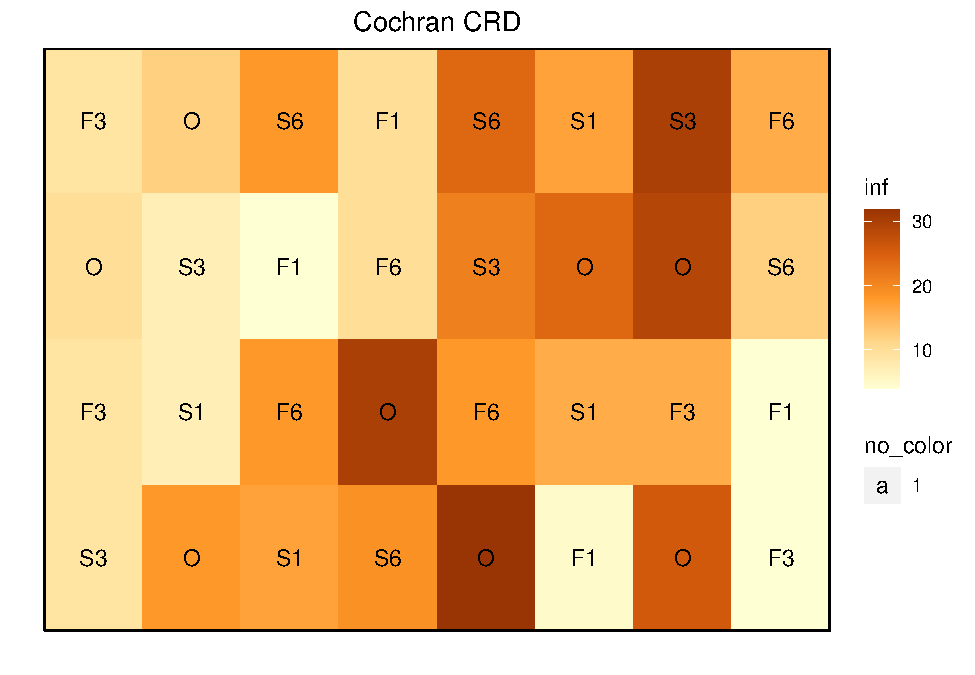
\includegraphics{Field-Trial-Spatial-Analysis-Guide_files/figure-latex/unnamed-chunk-60-1.pdf}

\begin{Shaded}
\begin{Highlighting}[]
\NormalTok{m\_crd }\OtherTok{\textless{}{-}} \FunctionTok{gls}\NormalTok{(inf }\SpecialCharTok{\textasciitilde{}}\NormalTok{ trt, }\AttributeTok{correlation =} \FunctionTok{corExp}\NormalTok{(}\AttributeTok{form =} \SpecialCharTok{\textasciitilde{}}\NormalTok{ row }\SpecialCharTok{+}\NormalTok{ col),}
             \AttributeTok{data =}\NormalTok{ cochran.crd)}
\end{Highlighting}
\end{Shaded}

\hypertarget{multi-way-factorials}{%
\subsection{Multi-way Factorials}\label{multi-way-factorials}}

Factorial experiments that are evaluating the effects of multiple crossed treatments are an extension of the linear mixed model (if your experimented uses RCBD), or the lienar model in the case of CRD.

The \emph{chinloy.fractionalfactorial} evaluates the effect of different fertilizer treatments (nitrogen, phosphorus, potassium, bagasse, and filter mud press) and concentrations on sugarcane yield. The levels of \{0,1,2\} for all variables indicate the relative concentrations of each fertilizer. Only 2-way interactions are being evaluated.

\begin{Shaded}
\begin{Highlighting}[]
\FunctionTok{data}\NormalTok{(chinloy.fractionalfactorial)}

\NormalTok{m\_factor }\OtherTok{\textless{}{-}} \FunctionTok{lme}\NormalTok{(yield }\SpecialCharTok{\textasciitilde{}}\NormalTok{ N }\SpecialCharTok{+}\NormalTok{ P }\SpecialCharTok{+}\NormalTok{ K }\SpecialCharTok{+}\NormalTok{ B }\SpecialCharTok{+}\NormalTok{ F }\SpecialCharTok{+}\NormalTok{ N}\SpecialCharTok{:}\NormalTok{P }\SpecialCharTok{+}\NormalTok{ N}\SpecialCharTok{:}\NormalTok{K }\SpecialCharTok{+}\NormalTok{ N}\SpecialCharTok{:}\NormalTok{B }\SpecialCharTok{+}\NormalTok{ N}\SpecialCharTok{:}\NormalTok{F, }
          \AttributeTok{random =} \SpecialCharTok{\textasciitilde{}} \DecValTok{1}\SpecialCharTok{|}\NormalTok{block, }
          \AttributeTok{correlation =} \FunctionTok{corMatern}\NormalTok{(}\AttributeTok{form =} \SpecialCharTok{\textasciitilde{}}\NormalTok{row }\SpecialCharTok{+}\NormalTok{ col), }
          \AttributeTok{data =}\NormalTok{ chinloy.fractionalfactorial)}
\end{Highlighting}
\end{Shaded}

\hypertarget{alpha-lattice}{%
\subsection{Alpha lattice}\label{alpha-lattice}}

The \emph{burgueno.alpha} data set uses an incomplete block alpha design with 16 treatment levels, 12 blocks and 3 reps.

\begin{Shaded}
\begin{Highlighting}[]
\FunctionTok{data}\NormalTok{(burgueno.alpha)}

\FunctionTok{ggdesplot}\NormalTok{(burgueno.alpha, yield }\SpecialCharTok{\textasciitilde{}}\NormalTok{ col}\SpecialCharTok{*}\NormalTok{row, }\AttributeTok{out1 =}\NormalTok{ block, }\AttributeTok{out2 =}\NormalTok{ rep, }
        \AttributeTok{text =}\NormalTok{ gen, }\AttributeTok{cex =} \DecValTok{1}\NormalTok{, }\AttributeTok{col.regions =}\NormalTok{ autumn, }
        \AttributeTok{main =} \StringTok{"Burgueno Alpha Lattice"}\NormalTok{)}
\end{Highlighting}
\end{Shaded}

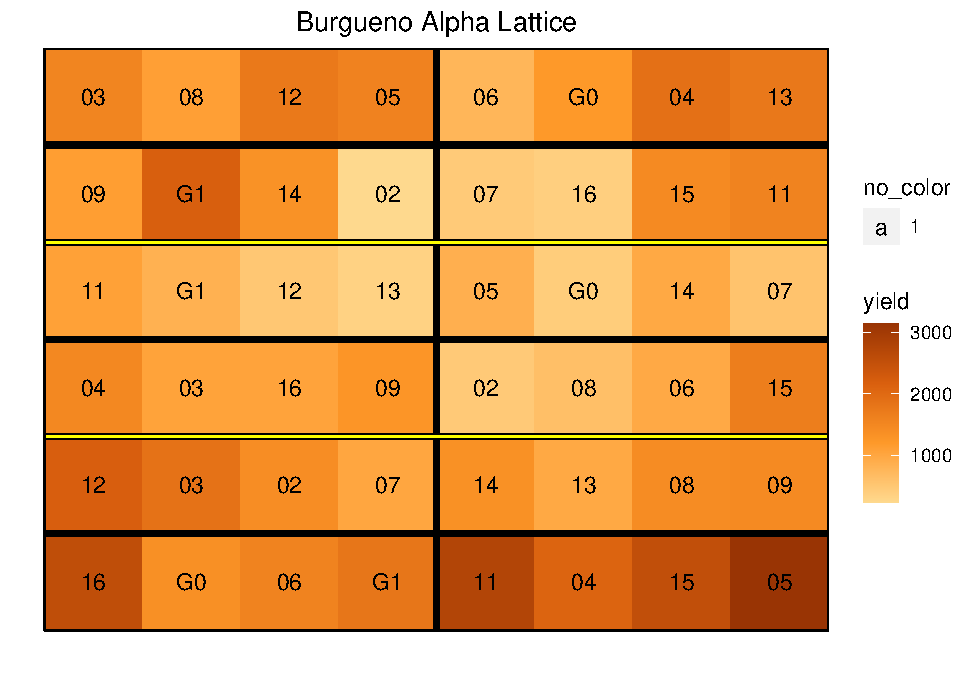
\includegraphics{Field-Trial-Spatial-Analysis-Guide_files/figure-latex/unnamed-chunk-62-1.pdf}

\begin{Shaded}
\begin{Highlighting}[]
\CommentTok{\# complicated asreml code in example}

\NormalTok{m\_alpha }\OtherTok{\textless{}{-}} \FunctionTok{lme}\NormalTok{(yield }\SpecialCharTok{\textasciitilde{}}\NormalTok{ gen,}
               \AttributeTok{random =} \SpecialCharTok{\textasciitilde{}} \DecValTok{1}\SpecialCharTok{|}\NormalTok{rep}\SpecialCharTok{/}\NormalTok{block,}
               \AttributeTok{data =}\NormalTok{ burgueno.alpha)}

\NormalTok{m\_alpha\_IBD  }\OtherTok{\textless{}{-}} \FunctionTok{remlf90}\NormalTok{(}\AttributeTok{fixed  =}\NormalTok{ yield }\SpecialCharTok{\textasciitilde{}}\NormalTok{ gen,}
                      \AttributeTok{random =} \SpecialCharTok{\textasciitilde{}}\NormalTok{ block,}
                      \AttributeTok{spatial =} \FunctionTok{list}\NormalTok{(}\AttributeTok{model =} \StringTok{\textquotesingle{}AR\textquotesingle{}}\NormalTok{, }
                                 \AttributeTok{coord =}\NormalTok{ burgueno.alpha[, }\FunctionTok{c}\NormalTok{(}\StringTok{\textquotesingle{}col\textquotesingle{}}\NormalTok{,}\StringTok{\textquotesingle{}row\textquotesingle{}}\NormalTok{)]), }
                      \AttributeTok{data =}\NormalTok{ burgueno.alpha)}
\end{Highlighting}
\end{Shaded}

\begin{verbatim}
Warning: 'as(<dsCMatrix>, "dgTMatrix")' is deprecated.
Use 'as(as(., "generalMatrix"), "TsparseMatrix")' instead.
See help("Deprecated") and help("Matrix-deprecated").

Warning: 'as(<dsCMatrix>, "dgTMatrix")' is deprecated.
Use 'as(as(., "generalMatrix"), "TsparseMatrix")' instead.
See help("Deprecated") and help("Matrix-deprecated").

Warning: 'as(<dsCMatrix>, "dgTMatrix")' is deprecated.
Use 'as(as(., "generalMatrix"), "TsparseMatrix")' instead.
See help("Deprecated") and help("Matrix-deprecated").

Warning: 'as(<dsCMatrix>, "dgTMatrix")' is deprecated.
Use 'as(as(., "generalMatrix"), "TsparseMatrix")' instead.
See help("Deprecated") and help("Matrix-deprecated").

Warning: 'as(<dsCMatrix>, "dgTMatrix")' is deprecated.
Use 'as(as(., "generalMatrix"), "TsparseMatrix")' instead.
See help("Deprecated") and help("Matrix-deprecated").

Warning: 'as(<dsCMatrix>, "dgTMatrix")' is deprecated.
Use 'as(as(., "generalMatrix"), "TsparseMatrix")' instead.
See help("Deprecated") and help("Matrix-deprecated").

Warning: 'as(<dsCMatrix>, "dgTMatrix")' is deprecated.
Use 'as(as(., "generalMatrix"), "TsparseMatrix")' instead.
See help("Deprecated") and help("Matrix-deprecated").

Warning: 'as(<dsCMatrix>, "dgTMatrix")' is deprecated.
Use 'as(as(., "generalMatrix"), "TsparseMatrix")' instead.
See help("Deprecated") and help("Matrix-deprecated").

Warning: 'as(<dsCMatrix>, "dgTMatrix")' is deprecated.
Use 'as(as(., "generalMatrix"), "TsparseMatrix")' instead.
See help("Deprecated") and help("Matrix-deprecated").

Warning: 'as(<dsCMatrix>, "dgTMatrix")' is deprecated.
Use 'as(as(., "generalMatrix"), "TsparseMatrix")' instead.
See help("Deprecated") and help("Matrix-deprecated").

Warning: 'as(<dsCMatrix>, "dgTMatrix")' is deprecated.
Use 'as(as(., "generalMatrix"), "TsparseMatrix")' instead.
See help("Deprecated") and help("Matrix-deprecated").

Warning: 'as(<dsCMatrix>, "dgTMatrix")' is deprecated.
Use 'as(as(., "generalMatrix"), "TsparseMatrix")' instead.
See help("Deprecated") and help("Matrix-deprecated").

Warning: 'as(<dsCMatrix>, "dgTMatrix")' is deprecated.
Use 'as(as(., "generalMatrix"), "TsparseMatrix")' instead.
See help("Deprecated") and help("Matrix-deprecated").

Warning: 'as(<dsCMatrix>, "dgTMatrix")' is deprecated.
Use 'as(as(., "generalMatrix"), "TsparseMatrix")' instead.
See help("Deprecated") and help("Matrix-deprecated").

Warning: 'as(<dsCMatrix>, "dgTMatrix")' is deprecated.
Use 'as(as(., "generalMatrix"), "TsparseMatrix")' instead.
See help("Deprecated") and help("Matrix-deprecated").

Warning: 'as(<dsCMatrix>, "dgTMatrix")' is deprecated.
Use 'as(as(., "generalMatrix"), "TsparseMatrix")' instead.
See help("Deprecated") and help("Matrix-deprecated").
\end{verbatim}

\begin{verbatim}
Warning in parse_results(file.path(tmpdir, "solutions"), effects, mf, reml.out,
: The algorithm did not converge
\end{verbatim}

\begin{verbatim}
Warning: 'as(<dsCMatrix>, "dgTMatrix")' is deprecated.
Use 'as(as(., "generalMatrix"), "TsparseMatrix")' instead.
See help("Deprecated") and help("Matrix-deprecated").

Warning: 'as(<dsCMatrix>, "dgTMatrix")' is deprecated.
Use 'as(as(., "generalMatrix"), "TsparseMatrix")' instead.
See help("Deprecated") and help("Matrix-deprecated").

Warning: 'as(<dsCMatrix>, "dgTMatrix")' is deprecated.
Use 'as(as(., "generalMatrix"), "TsparseMatrix")' instead.
See help("Deprecated") and help("Matrix-deprecated").

Warning: 'as(<dsCMatrix>, "dgTMatrix")' is deprecated.
Use 'as(as(., "generalMatrix"), "TsparseMatrix")' instead.
See help("Deprecated") and help("Matrix-deprecated").

Warning: 'as(<dsCMatrix>, "dgTMatrix")' is deprecated.
Use 'as(as(., "generalMatrix"), "TsparseMatrix")' instead.
See help("Deprecated") and help("Matrix-deprecated").

Warning: 'as(<dsCMatrix>, "dgTMatrix")' is deprecated.
Use 'as(as(., "generalMatrix"), "TsparseMatrix")' instead.
See help("Deprecated") and help("Matrix-deprecated").

Warning: 'as(<dsCMatrix>, "dgTMatrix")' is deprecated.
Use 'as(as(., "generalMatrix"), "TsparseMatrix")' instead.
See help("Deprecated") and help("Matrix-deprecated").

Warning: 'as(<dsCMatrix>, "dgTMatrix")' is deprecated.
Use 'as(as(., "generalMatrix"), "TsparseMatrix")' instead.
See help("Deprecated") and help("Matrix-deprecated").
\end{verbatim}

\begin{verbatim}
Warning in parse_results(file.path(tmpdir, "solutions"), effects, mf, reml.out,
: The algorithm did not converge
\end{verbatim}

\begin{verbatim}
Warning: 'as(<dsCMatrix>, "dgTMatrix")' is deprecated.
Use 'as(as(., "generalMatrix"), "TsparseMatrix")' instead.
See help("Deprecated") and help("Matrix-deprecated").

Warning: 'as(<dsCMatrix>, "dgTMatrix")' is deprecated.
Use 'as(as(., "generalMatrix"), "TsparseMatrix")' instead.
See help("Deprecated") and help("Matrix-deprecated").

Warning: 'as(<dsCMatrix>, "dgTMatrix")' is deprecated.
Use 'as(as(., "generalMatrix"), "TsparseMatrix")' instead.
See help("Deprecated") and help("Matrix-deprecated").

Warning: 'as(<dsCMatrix>, "dgTMatrix")' is deprecated.
Use 'as(as(., "generalMatrix"), "TsparseMatrix")' instead.
See help("Deprecated") and help("Matrix-deprecated").

Warning: 'as(<dsCMatrix>, "dgTMatrix")' is deprecated.
Use 'as(as(., "generalMatrix"), "TsparseMatrix")' instead.
See help("Deprecated") and help("Matrix-deprecated").

Warning: 'as(<dsCMatrix>, "dgTMatrix")' is deprecated.
Use 'as(as(., "generalMatrix"), "TsparseMatrix")' instead.
See help("Deprecated") and help("Matrix-deprecated").

Warning: 'as(<dsCMatrix>, "dgTMatrix")' is deprecated.
Use 'as(as(., "generalMatrix"), "TsparseMatrix")' instead.
See help("Deprecated") and help("Matrix-deprecated").

Warning: 'as(<dsCMatrix>, "dgTMatrix")' is deprecated.
Use 'as(as(., "generalMatrix"), "TsparseMatrix")' instead.
See help("Deprecated") and help("Matrix-deprecated").
\end{verbatim}

\hypertarget{latin-square}{%
\subsection{Latin square}\label{latin-square}}

Latin is a special example of a lattice experiment where each treatment occurs in each row and in each column. As a result, the row and column effects are used to model spatial effects.

The *cochran.latin** data set examines the effect of an ``operator'' (a person) on the difference between the true plot height and operator-measured height (of wheat plots).

\begin{Shaded}
\begin{Highlighting}[]
\FunctionTok{data}\NormalTok{(cochran.latin)}

\NormalTok{cochran.latin }\OtherTok{\textless{}{-}} \FunctionTok{transform}\NormalTok{(cochran.latin, }\AttributeTok{rowf =} \FunctionTok{as.factor}\NormalTok{(row), }\AttributeTok{colf =} \FunctionTok{as.factor}\NormalTok{(col))}

\FunctionTok{ggdesplot}\NormalTok{(cochran.latin, diff }\SpecialCharTok{\textasciitilde{}}\NormalTok{ col}\SpecialCharTok{*}\NormalTok{row, }
        \AttributeTok{text =}\NormalTok{ operator, }\AttributeTok{cex =} \DecValTok{1}\NormalTok{, }\AttributeTok{col.regions =}\NormalTok{ vir, }
        \AttributeTok{main =} \StringTok{"Cochran Latin Square"}\NormalTok{)}
\end{Highlighting}
\end{Shaded}

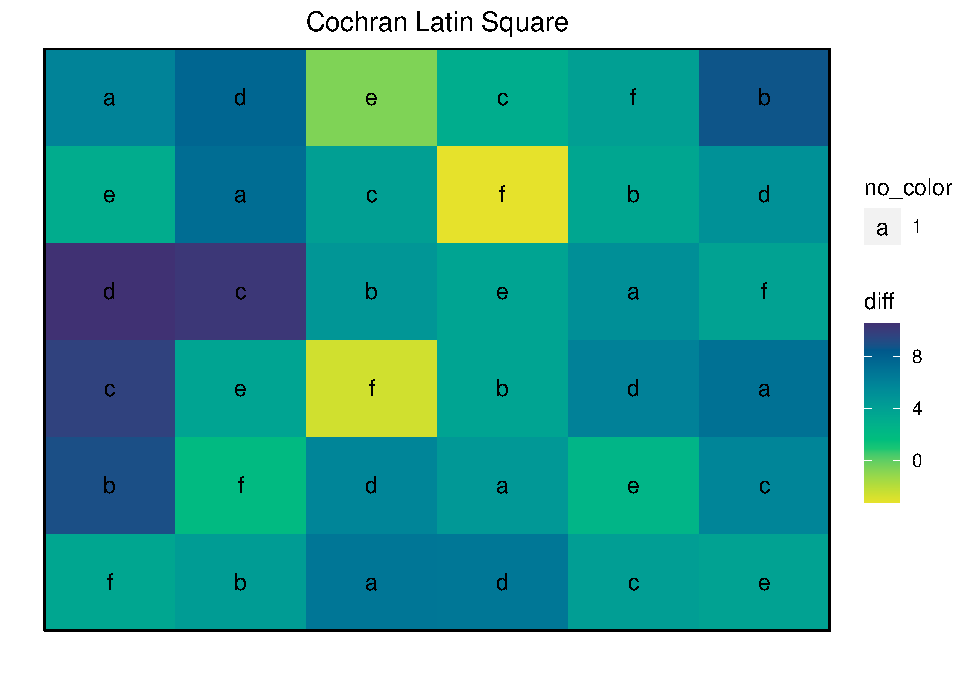
\includegraphics{Field-Trial-Spatial-Analysis-Guide_files/figure-latex/unnamed-chunk-63-1.pdf}

\begin{Shaded}
\begin{Highlighting}[]
\NormalTok{m\_latin }\OtherTok{\textless{}{-}} \FunctionTok{lmer}\NormalTok{(diff }\SpecialCharTok{\textasciitilde{}}\NormalTok{ operator }\SpecialCharTok{+}\NormalTok{ (}\DecValTok{1}\SpecialCharTok{|}\NormalTok{colf) }\SpecialCharTok{+}\NormalTok{ (}\DecValTok{1}\SpecialCharTok{|}\NormalTok{rowf),}
               \AttributeTok{data =}\NormalTok{ cochran.latin)}
\end{Highlighting}
\end{Shaded}

\hypertarget{split-plot}{%
\subsection{Split plot}\label{split-plot}}

The \emph{durban.splitplot} data set looks at the effect of fungicide on barley varieties. The main plot is fungicide (2 levels), and the sub plot is variety (70 levels). There are 4 blocks.

\begin{Shaded}
\begin{Highlighting}[]
\CommentTok{\# "bed" refers to the spatial position orthogonal to row (usually called \textquotesingle{}column\textquotesingle{})}
\FunctionTok{data}\NormalTok{(durban.splitplot)}

\FunctionTok{ggdesplot}\NormalTok{(durban.splitplot, yield}\SpecialCharTok{\textasciitilde{}}\NormalTok{bed}\SpecialCharTok{*}\NormalTok{row, }\AttributeTok{col.regions =}\NormalTok{ vir,}
          \AttributeTok{out1 =}\NormalTok{ block, }\AttributeTok{out2 =}\NormalTok{ fung, }\AttributeTok{num =}\NormalTok{ gen, }
          \AttributeTok{main =} \StringTok{"durban splitplot"}\NormalTok{)}
\end{Highlighting}
\end{Shaded}

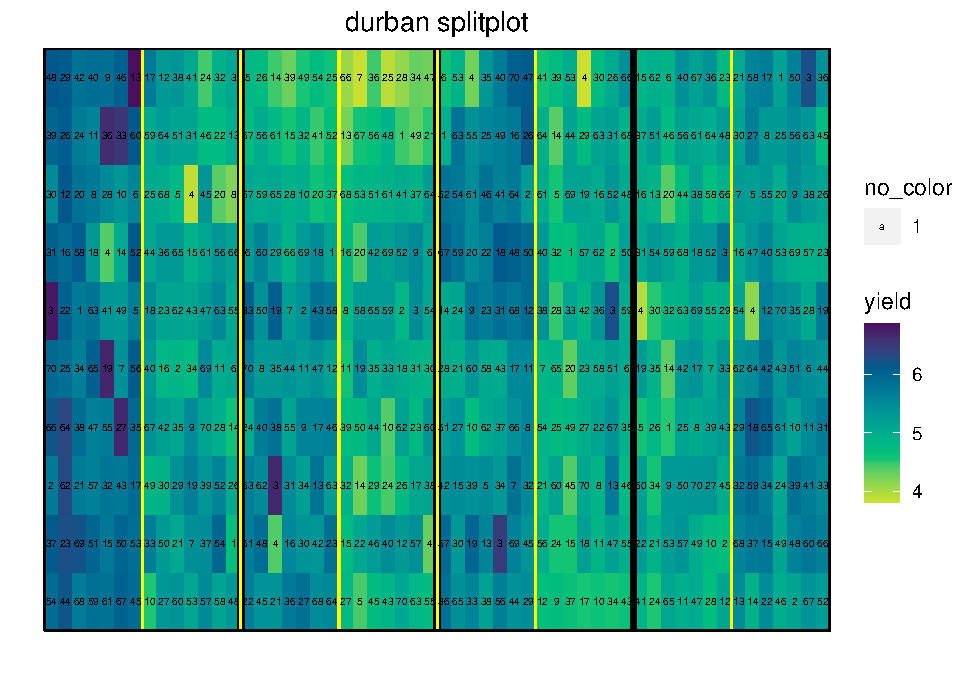
\includegraphics{Field-Trial-Spatial-Analysis-Guide_files/figure-latex/unnamed-chunk-64-1.pdf}

\begin{Shaded}
\begin{Highlighting}[]
\NormalTok{m\_sp }\OtherTok{\textless{}{-}} \FunctionTok{lme}\NormalTok{(yield }\SpecialCharTok{\textasciitilde{}}\NormalTok{ fung}\SpecialCharTok{*}\NormalTok{gen,}
            \AttributeTok{random =} \SpecialCharTok{\textasciitilde{}} \DecValTok{1}\SpecialCharTok{|}\NormalTok{block}\SpecialCharTok{/}\NormalTok{fung, }
            \AttributeTok{correlation =} \FunctionTok{corGaus}\NormalTok{(}\AttributeTok{form =} \SpecialCharTok{\textasciitilde{}}\NormalTok{ row }\SpecialCharTok{+}\NormalTok{ bed), }
            \AttributeTok{data =}\NormalTok{ durban.splitplot)}
\end{Highlighting}
\end{Shaded}

\hypertarget{split-split-plot}{%
\subsection{Split-split plot}\label{split-split-plot}}

The \emph{archbold.apple} data set of apple trees is examining the impact of spacing (the main plot), root stock (the split plot) and variety (the split-split plot) on fruit yield. There are 5 blocks.

\begin{Shaded}
\begin{Highlighting}[]
\FunctionTok{data}\NormalTok{(archbold.apple)}

\NormalTok{archbold.apple }\OtherTok{\textless{}{-}} \FunctionTok{transform}\NormalTok{(archbold.apple, }\AttributeTok{rep=}\FunctionTok{factor}\NormalTok{(rep), }\AttributeTok{spacing=}\FunctionTok{factor}\NormalTok{(spacing), }\AttributeTok{trt=}\FunctionTok{factor}\NormalTok{(trt),}
                 \AttributeTok{mainp =} \FunctionTok{factor}\NormalTok{(}\FunctionTok{paste}\NormalTok{(row, spacing, }\AttributeTok{sep=}\StringTok{""}\NormalTok{)),}
                 \AttributeTok{splitp =} \FunctionTok{factor}\NormalTok{(}\FunctionTok{paste}\NormalTok{(row, spacing, stock, }\AttributeTok{sep=}\StringTok{""}\NormalTok{)))}

\NormalTok{m\_ssp }\OtherTok{\textless{}{-}} \FunctionTok{lme}\NormalTok{(yield }\SpecialCharTok{\textasciitilde{}}\NormalTok{ spacing}\SpecialCharTok{*}\NormalTok{stock}\SpecialCharTok{*}\NormalTok{gen, }
             \AttributeTok{random =} \SpecialCharTok{\textasciitilde{}} \DecValTok{1}\SpecialCharTok{|}\NormalTok{rep}\SpecialCharTok{/}\NormalTok{mainp}\SpecialCharTok{/}\NormalTok{splitp, }
             \AttributeTok{correlation =} \FunctionTok{corExp}\NormalTok{(}\AttributeTok{form =} \SpecialCharTok{\textasciitilde{}}\NormalTok{ row }\SpecialCharTok{+}\NormalTok{ pos), }
             \AttributeTok{data =}\NormalTok{ archbold.apple, }\AttributeTok{na.action =}\NormalTok{ na.exclude)}
\end{Highlighting}
\end{Shaded}

\hypertarget{estimated-marginal-means}{%
\subsubsection{Estimated marginal means}\label{estimated-marginal-means}}

Emmeans can be extracted in the same way as previously described in \ref{rcbd-r}:

\begin{Shaded}
\begin{Highlighting}[]
\FunctionTok{library}\NormalTok{(emmeans)}
\NormalTok{preds }\OtherTok{\textless{}{-}} \FunctionTok{emmeans}\NormalTok{(m\_ssp, }\SpecialCharTok{\textasciitilde{}}\NormalTok{ gen }\SpecialCharTok{|}\NormalTok{ stock)}
\end{Highlighting}
\end{Shaded}

\begin{verbatim}
NOTE: Results may be misleading due to involvement in interactions
\end{verbatim}

\begin{Shaded}
\begin{Highlighting}[]
\FunctionTok{pairs}\NormalTok{(preds)}
\end{Highlighting}
\end{Shaded}

\begin{verbatim}
stock = M0007:
 contrast         estimate   SE df t.ratio p.value
 Golden - Redspur     22.7 14.3 24   1.589  0.1251

stock = MM106:
 contrast         estimate   SE df t.ratio p.value
 Golden - Redspur    -34.2 14.0 24  -2.434  0.0228

stock = MM111:
 contrast         estimate   SE df t.ratio p.value
 Golden - Redspur    -24.9 12.5 24  -1.985  0.0587

stock = Seedling:
 contrast         estimate   SE df t.ratio p.value
 Golden - Redspur     33.3 13.9 24   2.398  0.0246

Results are averaged over the levels of: spacing 
Degrees-of-freedom method: containment 
\end{verbatim}

\hypertarget{split-block}{%
\subsection{Split block}\label{split-block}}

also, over-dispersed count data

\begin{Shaded}
\begin{Highlighting}[]
\CommentTok{\# data(beall.webworms)  }
\CommentTok{\# under construction}
\end{Highlighting}
\end{Shaded}

\hypertarget{augmented-design}{%
\subsection{Augmented design}\label{augmented-design}}

\begin{Shaded}
\begin{Highlighting}[]
\CommentTok{\# lind \textless{}{-} read.csv("data/augmented\_lind.csv")}
\CommentTok{\# under construction}
\end{Highlighting}
\end{Shaded}

\hypertarget{model-extension-sas}{%
\chapter{Other Models - SAS}\label{model-extension-sas}}

\hypertarget{other-experimental-and-treatment-designs-1}{%
\section{Other Experimental and Treatment Designs}\label{other-experimental-and-treatment-designs-1}}

Spatial models can be extended to fit other experimental designs such as CRD, Lattice, and split plot or treatment designs such as factorials.

Below are minimal examples that omit several steps conducted in section \ref{rcbd-sas} (e.g.~fitting the empirical variogram) for brevity. Also, although spatial variance is incorporated into each example, we have not made an effort to ensure that each is the best fitting model for the data. The examples are intended to illustrate the correct syntax rather than the complete process of proper model fitting.

Unless indicated otherwise, these data are adapted from the R package agridat. Specific links to csv data files are given in the examples.

\hypertarget{completely-randomized-design-crd}{%
\subsection{Completely randomized design (CRD)}\label{completely-randomized-design-crd}}

Data: \href{https://raw.githubusercontent.com/IdahoAgStats/guide-to-field-trial-spatial-analysis/master/data/cochran_crd.csv}{cochran\_crd.csv}

This study investigated the effect of sulfur on controlling scab disease in potatoes and had seven treatments (trt) measuring the percent surface area infected (inf). Row and column indices are also given. The design was a completely randomized design with 8 control replications and 4 treatment replications.

Two possible methods of adjustment are shown: row column trend adjustment (as suggested in agridat), and a spline adjustment.

\begin{Shaded}
\begin{Highlighting}[]

\NormalTok{ods html close;}
\NormalTok{proc format;}
\NormalTok{invalue has\_NA}
\NormalTok{ \textquotesingle{}NA\textquotesingle{} = .;}
\NormalTok{run;}

\NormalTok{filename CRD url "https://raw.githubusercontent.com/IdahoAgStats/guide{-}to{-}field{-}trial{-}spatial{-}analysis/master/data/cochran\_crd.csv";}

\NormalTok{data CRD;}
\NormalTok{    infile CRD firstobs=2 delimiter=\textquotesingle{},\textquotesingle{};}
\NormalTok{    input inf trt$ row col;}
\NormalTok{    informat inf has\_NA.;}
\NormalTok{    if inf=. then delete;}
\NormalTok{run;}

\NormalTok{proc mixed data=crd;}
\NormalTok{    class trt;}
\NormalTok{    model inf=trt row col;}
\NormalTok{run;}

\NormalTok{proc glimmix data=crd;}
\NormalTok{    class trt;}
\NormalTok{    effect sp\_r = spline(row col);}
\NormalTok{    model inf=trt sp\_r;}
\NormalTok{    random row col/type=rsmooth;}
\NormalTok{run;}
 
\NormalTok{ods html; }
\end{Highlighting}
\end{Shaded}

\hypertarget{multi-way-factorials-1}{%
\subsection{Multi-way Factorials}\label{multi-way-factorials-1}}

Data: \href{https://raw.githubusercontent.com/IdahoAgStats/guide-to-field-trial-spatial-analysis/master/data/chinloy_fractionalfactorial.csv}{chinloy\_fractionalfactorial.csv}

Factorial experiments consider multiple treatments and their combinations. The study here evaluated the effect of 5 different fertilizer treatments (nitrogen, phosphorus, potassium, bagasse, and a filter mud press), each at various concentrations, on sugarcane yield. The levels of \{0,1,2\} indicate the relative concentrations of each fertilizer. Because all possible treatment combinations were too numerous, only a subset were used (fractional factorial) and only 2-way interactions with nitrogen are evaluated in the model. The treatments were laid out in a randomized complete block design (block).

A Gaussian spatial model is used below.

\begin{Shaded}
\begin{Highlighting}[]
\NormalTok{ods html close;}

\NormalTok{proc format;}
\NormalTok{invalue has\_NA}
\NormalTok{ \textquotesingle{}NA\textquotesingle{} = .;}
\NormalTok{run;}

\NormalTok{filename FACT url "https://raw.githubusercontent.com/IdahoAgStats/guide{-}to{-}field{-}trial{-}spatial{-}analysis/master/data/chinloy\_fractionalfactorial.csv";}

\NormalTok{data Factorial;}
\NormalTok{    infile FACT firstobs=2 delimiter=\textquotesingle{},\textquotesingle{};}
\NormalTok{    input yield block$ row col trt N P K B F;}
\NormalTok{    informat yield has\_NA.;}
\NormalTok{    if yield=. then delete;}
\NormalTok{run;}
 
\NormalTok{proc mixed data=Factorial maxiter=150;}
\NormalTok{    class block N P K B F;}
\NormalTok{    model yield = N P K B F N*P N*K N*B N*F/ ddfm=kr;}
\NormalTok{    random block;}
\NormalTok{    repeated/subject=intercept type=sp(gau) (row col) local;}
\NormalTok{    parms (6) (.25) (.21) (.1);}
\NormalTok{run;}

\NormalTok{ods html;}
\end{Highlighting}
\end{Shaded}

\hypertarget{alpha-lattice-1}{%
\subsection{Alpha lattice}\label{alpha-lattice-1}}

The \emph{burgueno.alpha} data set is set up as an incomplete block alpha design with 16 treatment levels (gen). There are 12 blocks, 2 each within 3 reps. The code below illustrates the layout of the reps and blocks. Two examples of spatial adjustment are shown: 1) assuming a Gaussian spatial adjustment, and 2) utilizing a spline adjustment.

\begin{Shaded}
\begin{Highlighting}[]
\NormalTok{proc format;}
\NormalTok{invalue has\_NA}
\NormalTok{ \textquotesingle{}NA\textquotesingle{} = .;}
\NormalTok{run;}

\NormalTok{filename ALPHA url "https://raw.githubusercontent.com/IdahoAgStats/guide{-}to{-}field{-}trial{-}spatial{-}analysis/master/data/burgueno\_alpha.csv";}

\NormalTok{data Lattice;}
\NormalTok{    infile ALPHA firstobs=2 delimiter=\textquotesingle{},\textquotesingle{};}
\NormalTok{    input rep$ block$ row col gen$ yield;}
\NormalTok{    informat yield has\_NA.;}
\NormalTok{    if yield=. then delete;}
\NormalTok{run;}

\NormalTok{proc sgplot data=Lattice;}
\NormalTok{    styleattrs datacolors=(cx990F26 cx99600F cx54990F);}
\NormalTok{    HEATMAPPARM y=row x=col COLORgroup=rep/ outline; }
\NormalTok{    refline 2.5 4.5/axis=y LINEATTRS=(color=black thickness=4) ;}
\NormalTok{title1 \textquotesingle{}Lattice: Layout of Reps\textquotesingle{};}

\NormalTok{run; }

\NormalTok{proc sgplot data=Lattice;}
\NormalTok{    styleattrs datacolors=(cx990F26 cxCC7A88 cxB33E52 cxE6B8BF}
\NormalTok{                           cx99600F cxCCAA7A cxB3823E cxE6D2B8 }
\NormalTok{                           cx54990F cxA3CC7A cx78B33E cxCFE6B8);}
\NormalTok{    HEATMAPPARM y=row x=col COLORgroup=block/ outline; }
\NormalTok{    refline 2.5 4.5/axis=y LINEATTRS=(color=black thickness=4) ;}
\NormalTok{    refline 4.5/axis=x LINEATTRS=(color=black thickness=4);}
\NormalTok{title1 \textquotesingle{}Lattice: Layout of Blocks\textquotesingle{};}
\NormalTok{run;}
\end{Highlighting}
\end{Shaded}

\begin{Shaded}
\begin{Highlighting}[]
\NormalTok{ods html close;}

\NormalTok{proc mixed data=Lattice ;}
\NormalTok{    class block rep gen;}
\NormalTok{    model yield = gen/ ddfm=kr;}
\NormalTok{    random rep block(rep);}
\NormalTok{    repeated/subject=intercept type=sp(gau) (row col) local;}
\NormalTok{    parms (4)(30711) (57790)(86861) (133229);}
\NormalTok{run;}

\NormalTok{proc glimmix data=Lattice ;}
\NormalTok{    class block rep gen;}
\NormalTok{    effect sp\_r = spline(row col);}
\NormalTok{    model yield = gen sp\_r/ ddfm=kr;}
\NormalTok{    random row col/type=rsmooth;}
\NormalTok{run;}

\NormalTok{ods html;}
\end{Highlighting}
\end{Shaded}

\hypertarget{latin-square-1}{%
\subsection{Latin square}\label{latin-square-1}}

Latin is a special example of a lattice experiment where each treatment occurs once in each row and in each column. As a result, the row and column effects are used to model spatial effects intrinsically.

The *cochran.latin** data set examines the effect of an 6 ``operators'' (persons) on the difference between the true plot height and operator-measured shoot height from 6 wheat plots. Each person measured the plots in a different order according to a Latin Square design. While this example is not strictly spatial in nature, it illustrates the setup for analysis.

\begin{Shaded}
\begin{Highlighting}[]
\NormalTok{ods html close;}

\NormalTok{proc format;}
\NormalTok{invalue has\_NA}
\NormalTok{ \textquotesingle{}NA\textquotesingle{} = .;}
\NormalTok{run;}

\NormalTok{filename LAT url "https://raw.githubusercontent.com/IdahoAgStats/guide{-}to{-}field{-}trial{-}spatial{-}analysis/master/data/cochran\_latin.csv";}

\NormalTok{data Latin;}
\NormalTok{    infile LAT firstobs=2 delimiter=\textquotesingle{},\textquotesingle{};}
\NormalTok{    input row col operator$ diff;}
\NormalTok{    informat diff has\_NA.;}
\NormalTok{    if diff=. then delete;}
\NormalTok{run;}

\NormalTok{proc mixed data=latin;}
\NormalTok{    class row col operator;}
\NormalTok{    model diff = operator;}
\NormalTok{    random row col;}
\NormalTok{run;}

\NormalTok{ods html;}
\end{Highlighting}
\end{Shaded}

\hypertarget{split-plot-1}{%
\subsection{Split plot}\label{split-plot-1}}

A split plot is a factorial treatment design with a restriction on the randomization of the factors. In this example, the \emph{durban.splitplot} data looks at the effect of two factors: fungicide and barley varieties. The study is set up with 4 blocks. Within each block, 2 fungicides are randomized as whole or main plots. Within each fungicide treatment, 70 barley varieties are then randomized separately as subplots. The resulting analysis then breaks out separate error terms for the whole plots and the subplots. The plots are arranged into 10 rows x 56 columns (`beds'). Spatial adjustment can then be introduced on top of this structure, if needed. The examples below illustrate a spherical spatial model adjustment and a spline adjustment.

\begin{Shaded}
\begin{Highlighting}[]
\NormalTok{ods html close;}

\NormalTok{proc format;}
\NormalTok{invalue has\_NA}
\NormalTok{ \textquotesingle{}NA\textquotesingle{} = .;}
\NormalTok{run;}

\NormalTok{filename SPLIT url "https://raw.githubusercontent.com/IdahoAgStats/guide{-}to{-}field{-}trial{-}spatial{-}analysis/master/data/durban\_splitplot.csv";}

\NormalTok{data splitplot;}
\NormalTok{    infile SPLIT firstobs=2 delimiter=\textquotesingle{},\textquotesingle{};}
\NormalTok{    input yield block$ gen$ fung$ row bed;}
\NormalTok{    informat yield has\_NA.;}
\NormalTok{    if yield=. then delete;}
\NormalTok{run;}

\NormalTok{proc mixed data=splitplot;}
\NormalTok{    class block gen fung row bed;}
\NormalTok{    model yield = fung gen fung*gen/outp=residuals;}
\NormalTok{    random block block*fung;}
\NormalTok{    repeated/subject=intercept type=sp(sph) (row bed) local;}
\NormalTok{    parms (7)(0.03)(0.03)(0.03) (0.01);}
\NormalTok{run;}

\NormalTok{proc glimmix data=splitplot;}
\NormalTok{    class block gen fung;}
\NormalTok{    effect sp\_r = spline(row bed);}
\NormalTok{    model yield = fung gen fung*gen sp\_r;}
\NormalTok{    random block block*fung;}
\NormalTok{    random row bed/type=rsmooth;}
\NormalTok{run;}

\NormalTok{ods html;}
\end{Highlighting}
\end{Shaded}

\hypertarget{split-split-plot-1}{%
\subsection{Split-split plot}\label{split-split-plot-1}}

Like the Split-Plot above, the Split-Split-Plot is a factorial design, this time with an additional restriction on the randomization. The \emph{archbold.apple} data used here describes the yield of apple trees under the impact of tree spacing (the whole or main plot), tree root stock (the split plot), and tree variety (the split-split plot). That is, 3 tree spacings are randomized in each block. Within those spacings, 4 root stocks are randomized separately, and then within each of those 2 varieties (`gen') are randomized. There are 5 blocks (`rep') and separate error terms for spacing, root stock, and variety are broken out in the analysis. In addition, we have row and column (`pos') information for the plots. This example uses a spline spatial adjustment.

\begin{Shaded}
\begin{Highlighting}[]
\NormalTok{ods html close;}

\NormalTok{proc format;}
\NormalTok{invalue has\_NA}
\NormalTok{ \textquotesingle{}NA\textquotesingle{} = .;}
\NormalTok{run;}

\NormalTok{filename SPLIT url "https://raw.githubusercontent.com/IdahoAgStats/guide{-}to{-}field{-}trial{-}spatial{-}analysis/master/data/archbold\_apple.csv";}

\NormalTok{data sp\_sp\_plot;}
\NormalTok{    infile SPLIT firstobs=2 delimiter=\textquotesingle{},\textquotesingle{};}
\NormalTok{    input rep$ row pos spacing$ stock$ gen$ yield trt;}
\NormalTok{    informat yield has\_NA.;}
\NormalTok{    if yield=. then delete;}
\NormalTok{run;}

\NormalTok{proc glimmix data=sp\_sp\_plot;}
\NormalTok{    class rep spacing stock gen;}
\NormalTok{    effect sp\_r = spline(row pos);}
\NormalTok{    model yield = spacing stock spacing*stock gen gen*spacing gen*stock gen*spacing*stock sp\_r;}
\NormalTok{    random rep rep*spacing rep*stock*spacing;}
\NormalTok{    random row pos/type=rsmooth;}
\NormalTok{run;}
 
\NormalTok{ ods html;}
\end{Highlighting}
\end{Shaded}

\hypertarget{split-block-or-strip-plot}{%
\subsection{Split block or Strip plot}\label{split-block-or-strip-plot}}

This study (\emph{little.splitblock}) investigated the effects of nitrogen rates (4 levels) and harvest dates (5 dates) on sugarbeet yields using 4 blocks. Similar to a Latin square, the split block design has two main factors defined in rows and columns. Within each block the rows and columns, each representing one of the factors, are independently randomized. The effect of this in the analysis of variance is to break out separate error terms and DF for each main effect as well as their interaction. In this example the spline spatial adjustment is demonstrated.

\begin{Shaded}
\begin{Highlighting}[]
\NormalTok{ods html close;}

\NormalTok{proc format;}
\NormalTok{invalue has\_NA}
\NormalTok{ \textquotesingle{}NA\textquotesingle{} = .;}
\NormalTok{run;}

\NormalTok{filename SPLITB url "https://raw.githubusercontent.com/IdahoAgStats/guide{-}to{-}field{-}trial{-}spatial{-}analysis/master/data/little\_splitblock.csv";}

\NormalTok{data sb;}
\NormalTok{    infile SPLITB firstobs=2 delimiter=\textquotesingle{},\textquotesingle{};}
\NormalTok{    input row col yield harvest nitro block$;}
\NormalTok{    informat yield has\_NA.;}
\NormalTok{    if yield=. then delete;}
\NormalTok{run;}

\NormalTok{proc glimmix data=sb;}
\NormalTok{    class harvest nitro block;}
\NormalTok{    effect sp\_r = spline(row col);}
\NormalTok{    model yield = harvest nitro harvest*nitro sp\_r;}
\NormalTok{    random block harvest*block nitro*block harvest*nitro*block;}
\NormalTok{    random row col/type=rsmooth;}
\NormalTok{run;}
 
\NormalTok{ods html;}
\end{Highlighting}
\end{Shaded}

\hypertarget{augmented-design-1}{%
\subsection{Augmented design}\label{augmented-design-1}}

The augmented experimental design occurs most commonly, if not exclusively, in plant breeding studies. It can be useful when the number of treatments is very large and the primary goal of the study is to rank or select genotypes that perform to a specified level. The number of treatments and/or limited materials often preclude complete replication of all treatments. To adjust for this, only a select set of genotypes, usually of known performance, are replicated in the design. The error estimated from these select genotypes is then utilized in the analysis to evaluate the remaining genotypes. \citet{Burgueno2018} have a very good discussion of this design and analysis of it. The example below uses their `P2' model and the reader is referred to \citet{Burgueno2018} for more details.

The data used here refer to a wheat genotype evaluation study carried out near Lind Washington. The study looked at 922 lines (`name'), of which, 8 were replicated known varieties. The P2 model, mentioned above, compares the averages of replicated lines to unreplicated lines. The data steps and procedures used below define these groups in an indicator variable named d2. The response variable, `yieldg', is converted to kilograms (`yieldkg') to facilitate computations and avoid numeric overflow errors due to large values.

\begin{Shaded}
\begin{Highlighting}[]
\NormalTok{filename AUG url "https://raw.githubusercontent.com/IdahoAgStats/guide{-}to{-}field{-}trial{-}spatial{-}analysis/master/data/augmented\_lind.csv";}

\NormalTok{PROC IMPORT OUT= WORK.augmented}
\NormalTok{     DATAFILE= AUG}
\NormalTok{     DBMS=CSV REPLACE;}
\NormalTok{     GETNAMES=YES;}
\NormalTok{     DATAROW=2; }
\NormalTok{RUN;}

\NormalTok{data augmented;}
\NormalTok{    set augmented;}
\NormalTok{    if yieldg = 999999 or yieldg=. then delete; /* Remove missing values */}
\NormalTok{    prow=prow*11.7; /*convert row and column indices to feet */}
\NormalTok{    pcol=pcol*5.5;}
\NormalTok{run;}

\NormalTok{proc freq noprint data=augmented;}
\NormalTok{    tables name/out=controls;}
\NormalTok{run;}

\NormalTok{data controls;}
\NormalTok{    set controls;}
\NormalTok{    if count \textgreater{}1;}
\NormalTok{run;}

\NormalTok{proc sort data=controls;}
\NormalTok{    by name;}
\NormalTok{run;}
     
\NormalTok{proc sort data=augmented;}
\NormalTok{    by name;}
\NormalTok{run;}

\NormalTok{data augmented;}
\NormalTok{    merge augmented controls;}
\NormalTok{    by name;}
\NormalTok{    if count=. then d2=2; /* Unreplicated */}
\NormalTok{    else d2=1;            /* Replicated */}
\NormalTok{    yieldkg=yieldg/1000;}
\NormalTok{run;}
\end{Highlighting}
\end{Shaded}

Following the steps described earlier, we first fit a base model, yieldkg = d2, to obtain residuals. We cannot use a base model of \texttt{yieldkg\ =\ name} because all the unreplicated lines will produce residual values of 0.

The residuals are then plotted in a heat map. This map shows evidence of spatial patterns and variability across the field.

\begin{Shaded}
\begin{Highlighting}[]
\NormalTok{PROC mixed data=augmented;}
\NormalTok{    class name d2;}
\NormalTok{    model yieldkg = d2/noint outp=residuals ddf=229 229;}
\NormalTok{    lsmeans d2;}
\NormalTok{    *lsmeans name(d2)/slice = d2;}
\NormalTok{run;}

\NormalTok{proc sgplot data=residuals;}
\NormalTok{    HEATMAPPARM y=pRow x=pCol COLORRESPONSE=resid/ colormodel=(cx014458 cx1E8C6E cxE1FE01); }
\NormalTok{title1 \textquotesingle{}Field Map\textquotesingle{};}
\NormalTok{run;}
\end{Highlighting}
\end{Shaded}

Model Information

Data Set

WORK.AUGMENTED

Dependent Variable

yieldkg

Covariance Structure

Diagonal

Estimation Method

REML

Residual Variance Method

Profile

Fixed Effects SE Method

Model-Based

Degrees of Freedom Method

Residual

Class Level Information

Class

Levels

Values

name

922

13X0828-0-0-1 13X0828-0-0-102 13X0828-0-0-105 13X0828-0-0-108 13X0828-0-0-109 13X0828-0-0-110 13X0828-0-0-15 13X0828-0-0-17 13X0828-0-0-18 13X0828-0-0-2 13X0828-0-0-24 13X0828-0-0-27 13X0828-0-0-31 13X0828-0-0-33 13X0828-0-0-36 13X0828-0-0-37 13X0828-0-0-40 13X0828-0-0-41 13X0828-0-0-42 13X0828-0-0-48 13X0828-0-0-49 13X0828-0-0-5 13X0828-0-0-52 13X0828-0-0-55 13X0828-0-0-6 13X0828-0-0-61 13X0828-0-0-62 13X0828-0-0-63 13X0828-0-0-66 13X0828-0-0-68 13X0828-0-0-7 13X0828-0-0-80 13X0828-0-0-81 13X0828-0-0-83 13X0828-0-0-9 13X0828-0-0-90 13X0828-0-0-91 13X0828-0-0-92 13X0828-0-0-94 13X0828-0-0-95 13X0828-0-0-97 13X0828-0-0-99 14X1001-0-0-1 14X1001-0-0-105 14X1001-0-0-106 14X1001-0-0-109 14X1001-0-0-11 14X1001-0-0-115 14X1001-0-0-116 14X1001-0-0-119 14X1001-0-0-12 14X1001-0-0-121 14X1001-0-0-122 14X1001-0-0-127 14X1001-0-0-128 14X1001-0-0-13 14X1001-0-0-130 14X1001-0-0-132 14X1001-0-0-134 14X1001-0-0-140 14X1001-0-0-141 14X1001-0-0-144 14X1001-0-0-146 14X1001-0-0-150 14X1001-0-0-156 14X1001-0-0-157 14X1001-0-0-158 14X1001-0-0-16 14X1001-0-0-160 14X1001-0-0-162 14X1001-0-0-164 14X1001-0-0-166 14X1001-0-0-167 14X1001-0-0-168 14X1001-0-0-169 14X1001-0-0-17 14X1001-0-0-174 14X1001-0-0-175 14X1001-0-0-176 14X1001-0-0-177 14X1001-0-0-178 14X1001-0-0-179 14X1001-0-0-181 14X1001-0-0-183 14X1001-0-0-185 14X1001-0-0-188 14X1001-0-0-193 14X1001-0-0-196 14X1001-0-0-197 14X1001-0-0-199 14X1001-0-0-20 14X1001-0-0-200 14X1001-0-0-203 14X1001-0-0-204 14X1001-0-0-205 14X1001-0-0-206 14X1001-0-0-207 14X1001-0-0-208 14X1001-0-0-209 14X1001-0-0-210 14X1001-0-0-211 14X1001-0-0-212 14X1001-0-0-213 14X1001-0-0-214 14X1001-0-0-219 14X1001-0-0-22 14X1001-0-0-223 14X1001-0-0-224 14X1001-0-0-225 14X1001-0-0-24 14X1001-0-0-25 14X1001-0-0-31 14X1001-0-0-33 14X1001-0-0-36 14X1001-0-0-38 14X1001-0-0-4 14X1001-0-0-41 14X1001-0-0-42 14X1001-0-0-43 14X1001-0-0-46 14X1001-0-0-47 14X1001-0-0-48 14X1001-0-0-49 14X1001-0-0-56 14X1001-0-0-57 14X1001-0-0-6 14X1001-0-0-60 14X1001-0-0-61 14X1001-0-0-64 14X1001-0-0-67 14X1001-0-0-68 14X1001-0-0-69 14X1001-0-0-77 14X1001-0-0-8 14X1001-0-0-81 14X1001-0-0-82 14X1001-0-0-87 14X1001-0-0-89 14X1001-0-0-92 14X1001-0-0-93 14X1001-0-0-97 14X1001-0-0-99 14X1003-0-0-1 14X1003-0-0-10 14X1003-0-0-102 14X1003-0-0-105 14X1003-0-0-106 14X1003-0-0-108 14X1003-0-0-110 14X1003-0-0-115 14X1003-0-0-121 14X1003-0-0-122 14X1003-0-0-124 14X1003-0-0-125 14X1003-0-0-127 14X1003-0-0-13 14X1003-0-0-130 14X1003-0-0-133 14X1003-0-0-140 14X1003-0-0-141 14X1003-0-0-146 14X1003-0-0-147 14X1003-0-0-149 14X1003-0-0-16 14X1003-0-0-167 14X1003-0-0-172 14X1003-0-0-175 14X1003-0-0-176 14X1003-0-0-177 14X1003-0-0-178 14X1003-0-0-18 14X1003-0-0-180 14X1003-0-0-181 14X1003-0-0-182 14X1003-0-0-185 14X1003-0-0-186 14X1003-0-0-190 14X1003-0-0-194 14X1003-0-0-195 14X1003-0-0-196 14X1003-0-0-198 14X1003-0-0-2 14X1003-0-0-20 14X1003-0-0-204 14X1003-0-0-21 14X1003-0-0-24 14X1003-0-0-27 14X1003-0-0-28 14X1003-0-0-30 14X1003-0-0-38 14X1003-0-0-41 14X1003-0-0-42 14X1003-0-0-44 14X1003-0-0-46 14X1003-0-0-47 14X1003-0-0-48 14X1003-0-0-49 14X1003-0-0-5 14X1003-0-0-50 14X1003-0-0-51 14X1003-0-0-52 14X1003-0-0-53 14X1003-0-0-54 14X1003-0-0-55 14X1003-0-0-56 14X1003-0-0-6 14X1003-0-0-60 14X1003-0-0-65 14X1003-0-0-66 14X1003-0-0-67 14X1003-0-0-68 14X1003-0-0-70 14X1003-0-0-71 14X1003-0-0-72 14X1003-0-0-73 14X1003-0-0-77 14X1003-0-0-8 14X1003-0-0-83 14X1003-0-0-86 14X1003-0-0-88 14X1003-0-0-92 14X1007-0-0-100 14X1007-0-0-101 14X1007-0-0-104 14X1007-0-0-109 14X1007-0-0-11 14X1007-0-0-111 14X1007-0-0-114 14X1007-0-0-115 14X1007-0-0-120 14X1007-0-0-122 14X1007-0-0-13 14X1007-0-0-16 14X1007-0-0-17 14X1007-0-0-20 14X1007-0-0-21 14X1007-0-0-25 14X1007-0-0-27 14X1007-0-0-29 14X1007-0-0-3 14X1007-0-0-31 14X1007-0-0-33 14X1007-0-0-37 14X1007-0-0-41 14X1007-0-0-47 14X1007-0-0-5 14X1007-0-0-50 14X1007-0-0-53 14X1007-0-0-54 14X1007-0-0-55 14X1007-0-0-59 14X1007-0-0-6 14X1007-0-0-61 14X1007-0-0-65 14X1007-0-0-68 14X1007-0-0-71 14X1007-0-0-72 14X1007-0-0-74 14X1007-0-0-77 14X1007-0-0-79 14X1007-0-0-86 14X1007-0-0-88 14X1007-0-0-9 14X1007-0-0-90 14X1007-0-0-91 14X1007-0-0-92 14X1007-0-0-94 14X1007-0-0-96 14X1007-0-0-98 14X1008-0-0-1 14X1008-0-0-10 14X1008-0-0-11 14X1008-0-0-14 14X1008-0-0-17 14X1008-0-0-2 14X1008-0-0-21 14X1008-0-0-22 14X1008-0-0-26 14X1008-0-0-28 14X1008-0-0-32 14X1008-0-0-33 14X1008-0-0-34 14X1008-0-0-4 14X1008-0-0-40 14X1008-0-0-42 14X1008-0-0-45 14X1008-0-0-46 14X1008-0-0-47 14X1008-0-0-48 14X1008-0-0-49 14X1008-0-0-5 14X1008-0-0-50 14X1008-0-0-54 14X1008-0-0-6 14X1008-0-0-61 14X1008-0-0-65 14X1008-0-0-7 14X1008-0-0-77 14X1008-0-0-78 14X1008-0-0-8 14X1008-0-0-82 14X1008-0-0-83 14X1008-0-0-85 14X1008-0-0-9 14X1022-0-0-12 14X1022-0-0-16 14X1022-0-0-2 14X1022-0-0-39 14X1022-0-0-43 14X1022-0-0-46 14X1022-0-0-49 14X1022-0-0-52 14X1022-0-0-53 14X1022-0-0-56 14X1022-0-0-59 14X1022-0-0-60 14X1022-0-0-61 14X1022-0-0-64 14X1022-0-0-66 14X1022-0-0-68 14X1022-0-0-70 14X1022-0-0-72 14X1022-0-0-76 14X1022-0-0-78 14X1023-0-0-18 14X1023-0-0-30 14X1023-0-0-33 14X1023-0-0-38 14X1023-0-0-39 14X1023-0-0-4 14X1023-0-0-45 14X1023-0-0-48 14X1023-0-0-49 14X1023-0-0-59 14X1023-0-0-70 14X1023-0-0-71 14X1023-0-0-73 14X1023-0-0-74 14X1023-0-0-75 14X1023-0-0-76 14X1023-0-0-78 14X1023-0-0-79 14X1023-0-0-80 14X1023-0-0-82 14X1023-0-0-85 14X1023-0-0-89 14X1023-0-0-90 14X1023-0-0-91 14X1027-0-0-104 14X1027-0-0-107 14X1027-0-0-11 14X1027-0-0-110 14X1027-0-0-112 14X1027-0-0-117 14X1027-0-0-121 14X1027-0-0-122 14X1027-0-0-123 14X1027-0-0-126 14X1027-0-0-128 14X1027-0-0-17 14X1027-0-0-22 14X1027-0-0-23 14X1027-0-0-25 14X1027-0-0-36 14X1027-0-0-37 14X1027-0-0-39 14X1027-0-0-4 14X1027-0-0-40 14X1027-0-0-43 14X1027-0-0-44 14X1027-0-0-45 14X1027-0-0-59 14X1027-0-0-62 14X1027-0-0-70 14X1027-0-0-77 14X1027-0-0-8 14X1027-0-0-82 14X1027-0-0-85 14X1027-0-0-92 14X1027-0-0-94 14X1030-0-0-1 14X1030-0-0-111 14X1030-0-0-112 14X1030-0-0-113 14X1030-0-0-120 14X1030-0-0-123 14X1030-0-0-128 14X1030-0-0-13 14X1030-0-0-131 14X1030-0-0-135 14X1030-0-0-14 14X1030-0-0-141 14X1030-0-0-145 14X1030-0-0-149 14X1030-0-0-16 14X1030-0-0-160 14X1030-0-0-161 14X1030-0-0-164 14X1030-0-0-168 14X1030-0-0-17 14X1030-0-0-176 14X1030-0-0-177 14X1030-0-0-18 14X1030-0-0-185 14X1030-0-0-188 14X1030-0-0-2 14X1030-0-0-215 14X1030-0-0-216 14X1030-0-0-220 14X1030-0-0-222 14X1030-0-0-226 14X1030-0-0-228 14X1030-0-0-25 14X1030-0-0-29 14X1030-0-0-36 14X1030-0-0-40 14X1030-0-0-54 14X1030-0-0-55 14X1030-0-0-68 14X1030-0-0-71 14X1030-0-0-72 14X1030-0-0-76 14X1030-0-0-77 14X1030-0-0-78 14X1030-0-0-80 14X1030-0-0-81 14X1030-0-0-84 14X1030-0-0-88 14X1030-0-0-93 14X1030-0-0-97 14X1031-0-0-105 14X1031-0-0-110 14X1031-0-0-112 14X1031-0-0-113 14X1031-0-0-114 14X1031-0-0-117 14X1031-0-0-120 14X1031-0-0-121 14X1031-0-0-125 14X1031-0-0-134 14X1031-0-0-136 14X1031-0-0-14 14X1031-0-0-141 14X1031-0-0-143 14X1031-0-0-147 14X1031-0-0-149 14X1031-0-0-16 14X1031-0-0-160 14X1031-0-0-161 14X1031-0-0-18 14X1031-0-0-2 14X1031-0-0-20 14X1031-0-0-21 14X1031-0-0-22 14X1031-0-0-23 14X1031-0-0-24 14X1031-0-0-28 14X1031-0-0-29 14X1031-0-0-3 14X1031-0-0-30 14X1031-0-0-32 14X1031-0-0-34 14X1031-0-0-35 14X1031-0-0-36 14X1031-0-0-4 14X1031-0-0-51 14X1031-0-0-52 14X1031-0-0-59 14X1031-0-0-6 14X1031-0-0-60 14X1031-0-0-64 14X1031-0-0-90 14X1031-0-0-93 14X1031-0-0-94 14X1031-0-0-96 14X1053-0-0-10 14X1053-0-0-103 14X1053-0-0-106 14X1053-0-0-107 14X1053-0-0-109 14X1053-0-0-110 14X1053-0-0-111 14X1053-0-0-118 14X1053-0-0-120 14X1053-0-0-124 14X1053-0-0-128 14X1053-0-0-13 14X1053-0-0-130 14X1053-0-0-131 14X1053-0-0-132 14X1053-0-0-133 14X1053-0-0-136 14X1053-0-0-137 14X1053-0-0-138 14X1053-0-0-139 14X1053-0-0-14 14X1053-0-0-142 14X1053-0-0-143 14X1053-0-0-146 14X1053-0-0-147 14X1053-0-0-149 14X1053-0-0-15 14X1053-0-0-151 14X1053-0-0-153 14X1053-0-0-154 14X1053-0-0-155 14X1053-0-0-157 14X1053-0-0-158 14X1053-0-0-162 14X1053-0-0-164 14X1053-0-0-166 14X1053-0-0-167 14X1053-0-0-168 14X1053-0-0-169 14X1053-0-0-170 14X1053-0-0-172 14X1053-0-0-174 14X1053-0-0-179 14X1053-0-0-180 14X1053-0-0-182 14X1053-0-0-19 14X1053-0-0-20 14X1053-0-0-23 14X1053-0-0-28 14X1053-0-0-29 14X1053-0-0-31 14X1053-0-0-33 14X1053-0-0-37 14X1053-0-0-4 14X1053-0-0-47 14X1053-0-0-5 14X1053-0-0-51 14X1053-0-0-52 14X1053-0-0-54 14X1053-0-0-55 14X1053-0-0-56 14X1053-0-0-58 14X1053-0-0-59 14X1053-0-0-6 14X1053-0-0-61 14X1053-0-0-63 14X1053-0-0-65 14X1053-0-0-66 14X1053-0-0-7 14X1053-0-0-71 14X1053-0-0-73 14X1053-0-0-74 14X1053-0-0-75 14X1053-0-0-76 14X1053-0-0-77 14X1053-0-0-78 14X1053-0-0-80 14X1053-0-0-81 14X1053-0-0-82 14X1053-0-0-87 14X1053-0-0-89 14X1053-0-0-9 14X1053-0-0-91 14X1053-0-0-92 14X1053-0-0-93 14X1053-0-0-97 14X1053-0-0-98 14X1054-0-0-1 14X1054-0-0-10 14X1054-0-0-14 14X1054-0-0-18 14X1054-0-0-2 14X1054-0-0-27 14X1054-0-0-28 14X1054-0-0-3 14X1054-0-0-31 14X1054-0-0-32 14X1054-0-0-34 14X1054-0-0-46 14X1054-0-0-5 14X1054-0-0-55 14X1054-0-0-6 14X1054-0-0-60 14X1054-0-0-61 14X1054-0-0-62 14X1054-0-0-64 14X1054-0-0-65 14X1054-0-0-9 14X1082-0-0-10 14X1082-0-0-12 14X1082-0-0-19 14X1082-0-0-20 14X1082-0-0-21 14X1082-0-0-22 14X1082-0-0-25 14X1082-0-0-27 14X1082-0-0-34 14X1082-0-0-7 14X1083-0-0-10 14X1083-0-0-100 14X1083-0-0-103 14X1083-0-0-104 14X1083-0-0-108 14X1083-0-0-112 14X1083-0-0-118 14X1083-0-0-12 14X1083-0-0-120 14X1083-0-0-129 14X1083-0-0-130 14X1083-0-0-134 14X1083-0-0-14 14X1083-0-0-140 14X1083-0-0-142 14X1083-0-0-146 14X1083-0-0-15 14X1083-0-0-157 14X1083-0-0-161 14X1083-0-0-162 14X1083-0-0-166 14X1083-0-0-167 14X1083-0-0-168 14X1083-0-0-174 14X1083-0-0-18 14X1083-0-0-183 14X1083-0-0-188 14X1083-0-0-191 14X1083-0-0-192 14X1083-0-0-197 14X1083-0-0-205 14X1083-0-0-213 14X1083-0-0-218 14X1083-0-0-221 14X1083-0-0-223 14X1083-0-0-230 14X1083-0-0-231 14X1083-0-0-234 14X1083-0-0-235 14X1083-0-0-238 14X1083-0-0-24 14X1083-0-0-243 14X1083-0-0-245 14X1083-0-0-251 14X1083-0-0-254 14X1083-0-0-256 14X1083-0-0-26 14X1083-0-0-260 14X1083-0-0-268 14X1083-0-0-3 14X1083-0-0-30 14X1083-0-0-33 14X1083-0-0-4 14X1083-0-0-46 14X1083-0-0-54 14X1083-0-0-59 14X1083-0-0-63 14X1083-0-0-65 14X1083-0-0-67 14X1083-0-0-71 14X1083-0-0-72 14X1083-0-0-76 14X1083-0-0-8 14X1083-0-0-86 14X1083-0-0-88 14X1083-0-0-9 14X1083-0-0-91 14X1083-0-0-93 14X1083-0-0-96 14X1083-0-0-99 14X1085-0-0-10 14X1085-0-0-11 14X1085-0-0-27 14X1085-0-0-34 14X1085-0-0-36 14X1085-0-0-56 14X1085-0-0-58 14X1085-0-0-59 14X1085-0-0-68 14X1085-0-0-71 14X1085-0-0-8 14X1085-0-0-83 14X1085-0-0-90 14X1085-0-0-93 14X1085-0-0-96 14X1098-0-0-10 14X1098-0-0-106 14X1098-0-0-109 14X1098-0-0-18 14X1098-0-0-30 14X1098-0-0-31 14X1098-0-0-34 14X1098-0-0-38 14X1098-0-0-39 14X1098-0-0-4 14X1098-0-0-41 14X1098-0-0-46 14X1098-0-0-48 14X1098-0-0-53 14X1098-0-0-54 14X1098-0-0-57 14X1098-0-0-7 14X1098-0-0-70 14X1098-0-0-72 14X1098-0-0-73 14X1098-0-0-79 14X1098-0-0-8 14X1098-0-0-81 14X1098-0-0-83 14X1098-0-0-94 14X1098-0-0-95 14X1098-0-0-96 14X1098-0-0-98 14X1103-0-0-104 14X1103-0-0-105 14X1103-0-0-106 14X1103-0-0-114 14X1103-0-0-115 14X1103-0-0-116 14X1103-0-0-117 14X1103-0-0-12 14X1103-0-0-120 14X1103-0-0-122 14X1103-0-0-124 14X1103-0-0-130 14X1103-0-0-131 14X1103-0-0-135 14X1103-0-0-136 14X1103-0-0-138 14X1103-0-0-141 14X1103-0-0-143 14X1103-0-0-146 14X1103-0-0-147 14X1103-0-0-148 14X1103-0-0-150 14X1103-0-0-155 14X1103-0-0-157 14X1103-0-0-159 14X1103-0-0-16 14X1103-0-0-162 14X1103-0-0-18 14X1103-0-0-27 14X1103-0-0-3 14X1103-0-0-31 14X1103-0-0-33 14X1103-0-0-37 14X1103-0-0-41 14X1103-0-0-42 14X1103-0-0-50 14X1103-0-0-51 14X1103-0-0-56 14X1103-0-0-58 14X1103-0-0-6 14X1103-0-0-63 14X1103-0-0-64 14X1103-0-0-68 14X1103-0-0-75 14X1103-0-0-76 14X1103-0-0-77 14X1103-0-0-79 14X1103-0-0-8 14X1103-0-0-80 14X1103-0-0-81 14X1103-0-0-83 14X1103-0-0-91 14X1103-0-0-96 14X1114-0-0-1 14X1114-0-0-101 14X1114-0-0-104 14X1114-0-0-105 14X1114-0-0-18 14X1114-0-0-23 14X1114-0-0-25 14X1114-0-0-26 14X1114-0-0-32 14X1114-0-0-36 14X1114-0-0-37 14X1114-0-0-4 14X1114-0-0-45 14X1114-0-0-48 14X1114-0-0-54 14X1114-0-0-60 14X1114-0-0-62 14X1114-0-0-64 14X1114-0-0-7 14X1114-0-0-73 14X1114-0-0-75 14X1114-0-0-79 14X1114-0-0-80 14X1114-0-0-84 14X1114-0-0-85 14X1114-0-0-90 14X1114-0-0-91 14X1114-0-0-92 14X1114-0-0-93 14X1114-0-0-97 14X1115-0-0-11 14X1115-0-0-14 14X1115-0-0-17 14X1115-0-0-2 14X1115-0-0-20 14X1115-0-0-21 14X1115-0-0-22 14X1115-0-0-25 14X1115-0-0-26 14X1115-0-0-28 14X1115-0-0-29 14X1115-0-0-31 14X1115-0-0-37 14X1115-0-0-41 14X1115-0-0-45 14X1115-0-0-48 14X1115-0-0-49 14X1115-0-0-5 14X1115-0-0-50 14X1115-0-0-51 14X1115-0-0-52 14X1115-0-0-53 14X1115-0-0-55 14X1115-0-0-56 14X1115-0-0-58 14X1115-0-0-6 14X1115-0-0-60 14X1115-0-0-62 14X1115-0-0-64 14X1115-0-0-66 14X1115-0-0-68 14X1115-0-0-69 14X1115-0-0-7 14X1115-0-0-73 14X1115-0-0-74 14X1115-0-0-77 14X1117-0-0-104 14X1117-0-0-114 14X1117-0-0-117 14X1117-0-0-12 14X1117-0-0-14 14X1117-0-0-23 14X1117-0-0-24 14X1117-0-0-26 14X1117-0-0-29 14X1117-0-0-3 14X1117-0-0-35 14X1117-0-0-36 14X1117-0-0-37 14X1117-0-0-38 14X1117-0-0-4 14X1117-0-0-43 14X1117-0-0-45 14X1117-0-0-46 14X1117-0-0-49 14X1117-0-0-50 14X1117-0-0-55 14X1117-0-0-6 14X1117-0-0-61 14X1117-0-0-64 14X1117-0-0-67 14X1117-0-0-69 14X1117-0-0-70 14X1117-0-0-72 14X1117-0-0-73 14X1117-0-0-74 14X1117-0-0-79 14X1117-0-0-8 14X1117-0-0-82 14X1117-0-0-83 14X1117-0-0-84 14X1117-0-0-85 14X1117-0-0-89 14X1117-0-0-9 14X1117-0-0-90 14X1117-0-0-92 14X1117-0-0-94 14X1117-0-0-96 14X1117-0-0-98 14X1117-0-0-99 14X1118-0-0-11 14X1118-0-0-119 14X1118-0-0-139 14X1118-0-0-14 14X1118-0-0-142 14X1118-0-0-15 14X1118-0-0-17 14X1118-0-0-173 14X1118-0-0-174 14X1118-0-0-178 14X1118-0-0-18 14X1118-0-0-188 14X1118-0-0-190 14X1118-0-0-194 14X1118-0-0-196 14X1118-0-0-198 14X1118-0-0-199 14X1118-0-0-20 14X1118-0-0-204 14X1118-0-0-208 14X1118-0-0-21 14X1118-0-0-22 14X1118-0-0-226 14X1118-0-0-23 14X1118-0-0-24 14X1118-0-0-26 14X1118-0-0-28 14X1118-0-0-32 14X1118-0-0-34 14X1118-0-0-35 14X1118-0-0-36 14X1118-0-0-37 14X1118-0-0-42 14X1118-0-0-43 14X1118-0-0-48 14X1118-0-0-50 14X1118-0-0-51 14X1118-0-0-52 14X1118-0-0-6 14X1118-0-0-64 14X1118-0-0-72 14X1118-0-0-92 14X1118-0-0-95 14X1118-0-0-99 ARS Crescent BRUEHL Bobtail Jasper LCS-HULK Otto Pritchett SY Banks SY Command

d2

2

1 2

Dimensions

Covariance Parameters

1

Columns in X

2

Columns in Z

0

Subjects

1

Max Obs per Subject

1151

Number of Observations

Number of Observations Read

1151

Number of Observations Used

1151

Number of Observations Not Used

0

Covariance Parameter Estimates

Cov Parm

Estimate

Residual

0.1200

Fit Statistics

-2 Res Log Likelihood

836.8

AIC (Smaller is Better)

838.8

AICC (Smaller is Better)

838.8

BIC (Smaller is Better)

843.8

Type 3 Tests of Fixed Effects

Effect

Num DF

Den DF

F Value

Pr \textgreater{} F

d2

2

229

20749.8

\textless.0001

Least Squares Means

Effect

d2

Estimate

StandardError

DF

t Value

Pr \textgreater{} \textbar t\textbar{}

d2

1

2.2018

0.02245

229

98.06

\textless.0001

d2

2

2.0471

0.01146

229

178.56

\textless.0001

The spatial variability evident in the residuals is then modeled as before. Only one model, power, is applicable to this data.

\begin{Shaded}
\begin{Highlighting}[]
\NormalTok{/*}
\NormalTok{proc variogram data=residuals plots=pairs(thr=50) ;}
\NormalTok{   compute novariogram nhclasses=60;}
\NormalTok{   coordinates xc=prow yc=pcol;}
\NormalTok{   var resid;}
\NormalTok{run;}

\NormalTok{proc variogram data=residuals plots(only)=(semivar);}
\NormalTok{   compute lagd=6.6 maxlags=20;}
\NormalTok{   coordinates xc=prow yc=pcol;}
\NormalTok{   var resid;}
\NormalTok{run;}

\NormalTok{*/}
\NormalTok{proc variogram data=residuals plots(only)=(fitplot);}
\NormalTok{   where yieldkg \^{}= .;}
\NormalTok{   coordinates xc=pcol yc=pRow;}
\NormalTok{   compute lagd=6.6 maxlags=25;}
\NormalTok{   model form=auto(mlist=(gau, exp, pow, sph) nest=1);}
\NormalTok{  var resid;}
\NormalTok{run;}
\end{Highlighting}
\end{Shaded}

Dependent Variable: Resid

Number of Observations Read

1151

Number of Observations Used

1151

Dependent Variable: Resid

Empirical Semivariogram

LagClass

PairCount

AverageDistance

Semivariance

0

0

.

.

1

1132

5.5

0.074

2

6442

13.4

0.091

3

4244

19.7

0.094

4

10058

25.8

0.101

5

11656

33.7

0.105

6

10288

39.4

0.105

7

12614

46.2

0.106

8

14102

51.9

0.110

9

20050

59.4

0.109

10

12140

65.9

0.114

11

21580

72.2

0.113

12

16310

79.2

0.115

13

21474

85.3

0.117

14

21548

92.8

0.117

15

20140

99.1

0.120

16

21671

106.1

0.118

17

18706

112.2

0.123

18

25052

118.9

0.122

19

18018

125.8

0.126

20

23362

131.9

0.126

21

19610

138.9

0.127

22

19241

144.7

0.131

23

22594

151.6

0.132

24

19995

158.3

0.136

25

18681

164.9

0.132

Dependent Variable: Resid

Angle: Omnidirectional

Semivariogram Model Fitting

Model

Selection from 4 form combinations

Fit Summary

Class

Model

WeightedSSE

AIC

Notes

1

Pow

55.66695

26.01277

Exp

70.00313

31.74160

Sph

77.47353

34.27651

Questionable fit

Gau

119.27905

45.06475

Semivariogram ModelFitting

Name

Power

Label

Pow

Model Information

Parameter

InitialValue

Nugget

0.0628

Slope

0.000443

Expon

0.5000

Optimization Information

Optimization Technique

Dual Quasi-Newton

Parameters in Optimization

3

Lower Boundaries

3

Upper Boundaries

1

Starting Values From

PROC

Parameter Estimates

Parameter

Estimate

ApproxStd Error

DF

t Value

ApproxPr \textgreater{} \textbar t\textbar{}

Gradient

Nugget

0.07429

0.000554

22

134.20

\textless.0001

-0.10262

Slope

0.005178

0

22

.

.

-0.74912

Expon

0.4748

0.002680

22

177.15

\textless.0001

-0.01655

Dependent Variable: Resid

Using the variogram model parameters estimated above, an adjusted model is then fit to the P2 hypothesis of \citet{Burgueno2018}. The residuals from this model show little, if any, spatial variability remains after adjustment.

\emph{Note: the lsmeans statement is commented out in this example to avoid a large amount of output.}

\begin{Shaded}
\begin{Highlighting}[]
\NormalTok{PROC mixed data=augmented;}
\NormalTok{    class name d2;}
\NormalTok{    model yieldkg = d2 name(d2)/outp=adjresiduals ddf=229 229;}
\NormalTok{    lsmeans d2;}
\NormalTok{    repeated/subject=intercept type=sp(pow)(prow pcol) local;}
\NormalTok{    ods output SolutionR =parms;}
\NormalTok{    parms (0.074) (0.0051)(0.475)  ;}
\NormalTok{    *lsmeans name(d2)/slice = d2;}
\NormalTok{run;}

\NormalTok{proc sgplot data=adjresiduals;}
\NormalTok{    HEATMAPPARM y=pRow x=pCol COLORRESPONSE=resid/ colormodel=(cx014458 cx1E8C6E cxE1FE01); }
\NormalTok{title1 \textquotesingle{}Field Map\textquotesingle{};}
\NormalTok{run;}
\end{Highlighting}
\end{Shaded}

Model Information

Data Set

WORK.AUGMENTED

Dependent Variable

yieldkg

Covariance Structure

Spatial Power

Subject Effect

Intercept

Estimation Method

REML

Residual Variance Method

Profile

Fixed Effects SE Method

Model-Based

Degrees of Freedom Method

Between-Within

Class Level Information

Class

Levels

Values

name

922

13X0828-0-0-1 13X0828-0-0-102 13X0828-0-0-105 13X0828-0-0-108 13X0828-0-0-109 13X0828-0-0-110 13X0828-0-0-15 13X0828-0-0-17 13X0828-0-0-18 13X0828-0-0-2 13X0828-0-0-24 13X0828-0-0-27 13X0828-0-0-31 13X0828-0-0-33 13X0828-0-0-36 13X0828-0-0-37 13X0828-0-0-40 13X0828-0-0-41 13X0828-0-0-42 13X0828-0-0-48 13X0828-0-0-49 13X0828-0-0-5 13X0828-0-0-52 13X0828-0-0-55 13X0828-0-0-6 13X0828-0-0-61 13X0828-0-0-62 13X0828-0-0-63 13X0828-0-0-66 13X0828-0-0-68 13X0828-0-0-7 13X0828-0-0-80 13X0828-0-0-81 13X0828-0-0-83 13X0828-0-0-9 13X0828-0-0-90 13X0828-0-0-91 13X0828-0-0-92 13X0828-0-0-94 13X0828-0-0-95 13X0828-0-0-97 13X0828-0-0-99 14X1001-0-0-1 14X1001-0-0-105 14X1001-0-0-106 14X1001-0-0-109 14X1001-0-0-11 14X1001-0-0-115 14X1001-0-0-116 14X1001-0-0-119 14X1001-0-0-12 14X1001-0-0-121 14X1001-0-0-122 14X1001-0-0-127 14X1001-0-0-128 14X1001-0-0-13 14X1001-0-0-130 14X1001-0-0-132 14X1001-0-0-134 14X1001-0-0-140 14X1001-0-0-141 14X1001-0-0-144 14X1001-0-0-146 14X1001-0-0-150 14X1001-0-0-156 14X1001-0-0-157 14X1001-0-0-158 14X1001-0-0-16 14X1001-0-0-160 14X1001-0-0-162 14X1001-0-0-164 14X1001-0-0-166 14X1001-0-0-167 14X1001-0-0-168 14X1001-0-0-169 14X1001-0-0-17 14X1001-0-0-174 14X1001-0-0-175 14X1001-0-0-176 14X1001-0-0-177 14X1001-0-0-178 14X1001-0-0-179 14X1001-0-0-181 14X1001-0-0-183 14X1001-0-0-185 14X1001-0-0-188 14X1001-0-0-193 14X1001-0-0-196 14X1001-0-0-197 14X1001-0-0-199 14X1001-0-0-20 14X1001-0-0-200 14X1001-0-0-203 14X1001-0-0-204 14X1001-0-0-205 14X1001-0-0-206 14X1001-0-0-207 14X1001-0-0-208 14X1001-0-0-209 14X1001-0-0-210 14X1001-0-0-211 14X1001-0-0-212 14X1001-0-0-213 14X1001-0-0-214 14X1001-0-0-219 14X1001-0-0-22 14X1001-0-0-223 14X1001-0-0-224 14X1001-0-0-225 14X1001-0-0-24 14X1001-0-0-25 14X1001-0-0-31 14X1001-0-0-33 14X1001-0-0-36 14X1001-0-0-38 14X1001-0-0-4 14X1001-0-0-41 14X1001-0-0-42 14X1001-0-0-43 14X1001-0-0-46 14X1001-0-0-47 14X1001-0-0-48 14X1001-0-0-49 14X1001-0-0-56 14X1001-0-0-57 14X1001-0-0-6 14X1001-0-0-60 14X1001-0-0-61 14X1001-0-0-64 14X1001-0-0-67 14X1001-0-0-68 14X1001-0-0-69 14X1001-0-0-77 14X1001-0-0-8 14X1001-0-0-81 14X1001-0-0-82 14X1001-0-0-87 14X1001-0-0-89 14X1001-0-0-92 14X1001-0-0-93 14X1001-0-0-97 14X1001-0-0-99 14X1003-0-0-1 14X1003-0-0-10 14X1003-0-0-102 14X1003-0-0-105 14X1003-0-0-106 14X1003-0-0-108 14X1003-0-0-110 14X1003-0-0-115 14X1003-0-0-121 14X1003-0-0-122 14X1003-0-0-124 14X1003-0-0-125 14X1003-0-0-127 14X1003-0-0-13 14X1003-0-0-130 14X1003-0-0-133 14X1003-0-0-140 14X1003-0-0-141 14X1003-0-0-146 14X1003-0-0-147 14X1003-0-0-149 14X1003-0-0-16 14X1003-0-0-167 14X1003-0-0-172 14X1003-0-0-175 14X1003-0-0-176 14X1003-0-0-177 14X1003-0-0-178 14X1003-0-0-18 14X1003-0-0-180 14X1003-0-0-181 14X1003-0-0-182 14X1003-0-0-185 14X1003-0-0-186 14X1003-0-0-190 14X1003-0-0-194 14X1003-0-0-195 14X1003-0-0-196 14X1003-0-0-198 14X1003-0-0-2 14X1003-0-0-20 14X1003-0-0-204 14X1003-0-0-21 14X1003-0-0-24 14X1003-0-0-27 14X1003-0-0-28 14X1003-0-0-30 14X1003-0-0-38 14X1003-0-0-41 14X1003-0-0-42 14X1003-0-0-44 14X1003-0-0-46 14X1003-0-0-47 14X1003-0-0-48 14X1003-0-0-49 14X1003-0-0-5 14X1003-0-0-50 14X1003-0-0-51 14X1003-0-0-52 14X1003-0-0-53 14X1003-0-0-54 14X1003-0-0-55 14X1003-0-0-56 14X1003-0-0-6 14X1003-0-0-60 14X1003-0-0-65 14X1003-0-0-66 14X1003-0-0-67 14X1003-0-0-68 14X1003-0-0-70 14X1003-0-0-71 14X1003-0-0-72 14X1003-0-0-73 14X1003-0-0-77 14X1003-0-0-8 14X1003-0-0-83 14X1003-0-0-86 14X1003-0-0-88 14X1003-0-0-92 14X1007-0-0-100 14X1007-0-0-101 14X1007-0-0-104 14X1007-0-0-109 14X1007-0-0-11 14X1007-0-0-111 14X1007-0-0-114 14X1007-0-0-115 14X1007-0-0-120 14X1007-0-0-122 14X1007-0-0-13 14X1007-0-0-16 14X1007-0-0-17 14X1007-0-0-20 14X1007-0-0-21 14X1007-0-0-25 14X1007-0-0-27 14X1007-0-0-29 14X1007-0-0-3 14X1007-0-0-31 14X1007-0-0-33 14X1007-0-0-37 14X1007-0-0-41 14X1007-0-0-47 14X1007-0-0-5 14X1007-0-0-50 14X1007-0-0-53 14X1007-0-0-54 14X1007-0-0-55 14X1007-0-0-59 14X1007-0-0-6 14X1007-0-0-61 14X1007-0-0-65 14X1007-0-0-68 14X1007-0-0-71 14X1007-0-0-72 14X1007-0-0-74 14X1007-0-0-77 14X1007-0-0-79 14X1007-0-0-86 14X1007-0-0-88 14X1007-0-0-9 14X1007-0-0-90 14X1007-0-0-91 14X1007-0-0-92 14X1007-0-0-94 14X1007-0-0-96 14X1007-0-0-98 14X1008-0-0-1 14X1008-0-0-10 14X1008-0-0-11 14X1008-0-0-14 14X1008-0-0-17 14X1008-0-0-2 14X1008-0-0-21 14X1008-0-0-22 14X1008-0-0-26 14X1008-0-0-28 14X1008-0-0-32 14X1008-0-0-33 14X1008-0-0-34 14X1008-0-0-4 14X1008-0-0-40 14X1008-0-0-42 14X1008-0-0-45 14X1008-0-0-46 14X1008-0-0-47 14X1008-0-0-48 14X1008-0-0-49 14X1008-0-0-5 14X1008-0-0-50 14X1008-0-0-54 14X1008-0-0-6 14X1008-0-0-61 14X1008-0-0-65 14X1008-0-0-7 14X1008-0-0-77 14X1008-0-0-78 14X1008-0-0-8 14X1008-0-0-82 14X1008-0-0-83 14X1008-0-0-85 14X1008-0-0-9 14X1022-0-0-12 14X1022-0-0-16 14X1022-0-0-2 14X1022-0-0-39 14X1022-0-0-43 14X1022-0-0-46 14X1022-0-0-49 14X1022-0-0-52 14X1022-0-0-53 14X1022-0-0-56 14X1022-0-0-59 14X1022-0-0-60 14X1022-0-0-61 14X1022-0-0-64 14X1022-0-0-66 14X1022-0-0-68 14X1022-0-0-70 14X1022-0-0-72 14X1022-0-0-76 14X1022-0-0-78 14X1023-0-0-18 14X1023-0-0-30 14X1023-0-0-33 14X1023-0-0-38 14X1023-0-0-39 14X1023-0-0-4 14X1023-0-0-45 14X1023-0-0-48 14X1023-0-0-49 14X1023-0-0-59 14X1023-0-0-70 14X1023-0-0-71 14X1023-0-0-73 14X1023-0-0-74 14X1023-0-0-75 14X1023-0-0-76 14X1023-0-0-78 14X1023-0-0-79 14X1023-0-0-80 14X1023-0-0-82 14X1023-0-0-85 14X1023-0-0-89 14X1023-0-0-90 14X1023-0-0-91 14X1027-0-0-104 14X1027-0-0-107 14X1027-0-0-11 14X1027-0-0-110 14X1027-0-0-112 14X1027-0-0-117 14X1027-0-0-121 14X1027-0-0-122 14X1027-0-0-123 14X1027-0-0-126 14X1027-0-0-128 14X1027-0-0-17 14X1027-0-0-22 14X1027-0-0-23 14X1027-0-0-25 14X1027-0-0-36 14X1027-0-0-37 14X1027-0-0-39 14X1027-0-0-4 14X1027-0-0-40 14X1027-0-0-43 14X1027-0-0-44 14X1027-0-0-45 14X1027-0-0-59 14X1027-0-0-62 14X1027-0-0-70 14X1027-0-0-77 14X1027-0-0-8 14X1027-0-0-82 14X1027-0-0-85 14X1027-0-0-92 14X1027-0-0-94 14X1030-0-0-1 14X1030-0-0-111 14X1030-0-0-112 14X1030-0-0-113 14X1030-0-0-120 14X1030-0-0-123 14X1030-0-0-128 14X1030-0-0-13 14X1030-0-0-131 14X1030-0-0-135 14X1030-0-0-14 14X1030-0-0-141 14X1030-0-0-145 14X1030-0-0-149 14X1030-0-0-16 14X1030-0-0-160 14X1030-0-0-161 14X1030-0-0-164 14X1030-0-0-168 14X1030-0-0-17 14X1030-0-0-176 14X1030-0-0-177 14X1030-0-0-18 14X1030-0-0-185 14X1030-0-0-188 14X1030-0-0-2 14X1030-0-0-215 14X1030-0-0-216 14X1030-0-0-220 14X1030-0-0-222 14X1030-0-0-226 14X1030-0-0-228 14X1030-0-0-25 14X1030-0-0-29 14X1030-0-0-36 14X1030-0-0-40 14X1030-0-0-54 14X1030-0-0-55 14X1030-0-0-68 14X1030-0-0-71 14X1030-0-0-72 14X1030-0-0-76 14X1030-0-0-77 14X1030-0-0-78 14X1030-0-0-80 14X1030-0-0-81 14X1030-0-0-84 14X1030-0-0-88 14X1030-0-0-93 14X1030-0-0-97 14X1031-0-0-105 14X1031-0-0-110 14X1031-0-0-112 14X1031-0-0-113 14X1031-0-0-114 14X1031-0-0-117 14X1031-0-0-120 14X1031-0-0-121 14X1031-0-0-125 14X1031-0-0-134 14X1031-0-0-136 14X1031-0-0-14 14X1031-0-0-141 14X1031-0-0-143 14X1031-0-0-147 14X1031-0-0-149 14X1031-0-0-16 14X1031-0-0-160 14X1031-0-0-161 14X1031-0-0-18 14X1031-0-0-2 14X1031-0-0-20 14X1031-0-0-21 14X1031-0-0-22 14X1031-0-0-23 14X1031-0-0-24 14X1031-0-0-28 14X1031-0-0-29 14X1031-0-0-3 14X1031-0-0-30 14X1031-0-0-32 14X1031-0-0-34 14X1031-0-0-35 14X1031-0-0-36 14X1031-0-0-4 14X1031-0-0-51 14X1031-0-0-52 14X1031-0-0-59 14X1031-0-0-6 14X1031-0-0-60 14X1031-0-0-64 14X1031-0-0-90 14X1031-0-0-93 14X1031-0-0-94 14X1031-0-0-96 14X1053-0-0-10 14X1053-0-0-103 14X1053-0-0-106 14X1053-0-0-107 14X1053-0-0-109 14X1053-0-0-110 14X1053-0-0-111 14X1053-0-0-118 14X1053-0-0-120 14X1053-0-0-124 14X1053-0-0-128 14X1053-0-0-13 14X1053-0-0-130 14X1053-0-0-131 14X1053-0-0-132 14X1053-0-0-133 14X1053-0-0-136 14X1053-0-0-137 14X1053-0-0-138 14X1053-0-0-139 14X1053-0-0-14 14X1053-0-0-142 14X1053-0-0-143 14X1053-0-0-146 14X1053-0-0-147 14X1053-0-0-149 14X1053-0-0-15 14X1053-0-0-151 14X1053-0-0-153 14X1053-0-0-154 14X1053-0-0-155 14X1053-0-0-157 14X1053-0-0-158 14X1053-0-0-162 14X1053-0-0-164 14X1053-0-0-166 14X1053-0-0-167 14X1053-0-0-168 14X1053-0-0-169 14X1053-0-0-170 14X1053-0-0-172 14X1053-0-0-174 14X1053-0-0-179 14X1053-0-0-180 14X1053-0-0-182 14X1053-0-0-19 14X1053-0-0-20 14X1053-0-0-23 14X1053-0-0-28 14X1053-0-0-29 14X1053-0-0-31 14X1053-0-0-33 14X1053-0-0-37 14X1053-0-0-4 14X1053-0-0-47 14X1053-0-0-5 14X1053-0-0-51 14X1053-0-0-52 14X1053-0-0-54 14X1053-0-0-55 14X1053-0-0-56 14X1053-0-0-58 14X1053-0-0-59 14X1053-0-0-6 14X1053-0-0-61 14X1053-0-0-63 14X1053-0-0-65 14X1053-0-0-66 14X1053-0-0-7 14X1053-0-0-71 14X1053-0-0-73 14X1053-0-0-74 14X1053-0-0-75 14X1053-0-0-76 14X1053-0-0-77 14X1053-0-0-78 14X1053-0-0-80 14X1053-0-0-81 14X1053-0-0-82 14X1053-0-0-87 14X1053-0-0-89 14X1053-0-0-9 14X1053-0-0-91 14X1053-0-0-92 14X1053-0-0-93 14X1053-0-0-97 14X1053-0-0-98 14X1054-0-0-1 14X1054-0-0-10 14X1054-0-0-14 14X1054-0-0-18 14X1054-0-0-2 14X1054-0-0-27 14X1054-0-0-28 14X1054-0-0-3 14X1054-0-0-31 14X1054-0-0-32 14X1054-0-0-34 14X1054-0-0-46 14X1054-0-0-5 14X1054-0-0-55 14X1054-0-0-6 14X1054-0-0-60 14X1054-0-0-61 14X1054-0-0-62 14X1054-0-0-64 14X1054-0-0-65 14X1054-0-0-9 14X1082-0-0-10 14X1082-0-0-12 14X1082-0-0-19 14X1082-0-0-20 14X1082-0-0-21 14X1082-0-0-22 14X1082-0-0-25 14X1082-0-0-27 14X1082-0-0-34 14X1082-0-0-7 14X1083-0-0-10 14X1083-0-0-100 14X1083-0-0-103 14X1083-0-0-104 14X1083-0-0-108 14X1083-0-0-112 14X1083-0-0-118 14X1083-0-0-12 14X1083-0-0-120 14X1083-0-0-129 14X1083-0-0-130 14X1083-0-0-134 14X1083-0-0-14 14X1083-0-0-140 14X1083-0-0-142 14X1083-0-0-146 14X1083-0-0-15 14X1083-0-0-157 14X1083-0-0-161 14X1083-0-0-162 14X1083-0-0-166 14X1083-0-0-167 14X1083-0-0-168 14X1083-0-0-174 14X1083-0-0-18 14X1083-0-0-183 14X1083-0-0-188 14X1083-0-0-191 14X1083-0-0-192 14X1083-0-0-197 14X1083-0-0-205 14X1083-0-0-213 14X1083-0-0-218 14X1083-0-0-221 14X1083-0-0-223 14X1083-0-0-230 14X1083-0-0-231 14X1083-0-0-234 14X1083-0-0-235 14X1083-0-0-238 14X1083-0-0-24 14X1083-0-0-243 14X1083-0-0-245 14X1083-0-0-251 14X1083-0-0-254 14X1083-0-0-256 14X1083-0-0-26 14X1083-0-0-260 14X1083-0-0-268 14X1083-0-0-3 14X1083-0-0-30 14X1083-0-0-33 14X1083-0-0-4 14X1083-0-0-46 14X1083-0-0-54 14X1083-0-0-59 14X1083-0-0-63 14X1083-0-0-65 14X1083-0-0-67 14X1083-0-0-71 14X1083-0-0-72 14X1083-0-0-76 14X1083-0-0-8 14X1083-0-0-86 14X1083-0-0-88 14X1083-0-0-9 14X1083-0-0-91 14X1083-0-0-93 14X1083-0-0-96 14X1083-0-0-99 14X1085-0-0-10 14X1085-0-0-11 14X1085-0-0-27 14X1085-0-0-34 14X1085-0-0-36 14X1085-0-0-56 14X1085-0-0-58 14X1085-0-0-59 14X1085-0-0-68 14X1085-0-0-71 14X1085-0-0-8 14X1085-0-0-83 14X1085-0-0-90 14X1085-0-0-93 14X1085-0-0-96 14X1098-0-0-10 14X1098-0-0-106 14X1098-0-0-109 14X1098-0-0-18 14X1098-0-0-30 14X1098-0-0-31 14X1098-0-0-34 14X1098-0-0-38 14X1098-0-0-39 14X1098-0-0-4 14X1098-0-0-41 14X1098-0-0-46 14X1098-0-0-48 14X1098-0-0-53 14X1098-0-0-54 14X1098-0-0-57 14X1098-0-0-7 14X1098-0-0-70 14X1098-0-0-72 14X1098-0-0-73 14X1098-0-0-79 14X1098-0-0-8 14X1098-0-0-81 14X1098-0-0-83 14X1098-0-0-94 14X1098-0-0-95 14X1098-0-0-96 14X1098-0-0-98 14X1103-0-0-104 14X1103-0-0-105 14X1103-0-0-106 14X1103-0-0-114 14X1103-0-0-115 14X1103-0-0-116 14X1103-0-0-117 14X1103-0-0-12 14X1103-0-0-120 14X1103-0-0-122 14X1103-0-0-124 14X1103-0-0-130 14X1103-0-0-131 14X1103-0-0-135 14X1103-0-0-136 14X1103-0-0-138 14X1103-0-0-141 14X1103-0-0-143 14X1103-0-0-146 14X1103-0-0-147 14X1103-0-0-148 14X1103-0-0-150 14X1103-0-0-155 14X1103-0-0-157 14X1103-0-0-159 14X1103-0-0-16 14X1103-0-0-162 14X1103-0-0-18 14X1103-0-0-27 14X1103-0-0-3 14X1103-0-0-31 14X1103-0-0-33 14X1103-0-0-37 14X1103-0-0-41 14X1103-0-0-42 14X1103-0-0-50 14X1103-0-0-51 14X1103-0-0-56 14X1103-0-0-58 14X1103-0-0-6 14X1103-0-0-63 14X1103-0-0-64 14X1103-0-0-68 14X1103-0-0-75 14X1103-0-0-76 14X1103-0-0-77 14X1103-0-0-79 14X1103-0-0-8 14X1103-0-0-80 14X1103-0-0-81 14X1103-0-0-83 14X1103-0-0-91 14X1103-0-0-96 14X1114-0-0-1 14X1114-0-0-101 14X1114-0-0-104 14X1114-0-0-105 14X1114-0-0-18 14X1114-0-0-23 14X1114-0-0-25 14X1114-0-0-26 14X1114-0-0-32 14X1114-0-0-36 14X1114-0-0-37 14X1114-0-0-4 14X1114-0-0-45 14X1114-0-0-48 14X1114-0-0-54 14X1114-0-0-60 14X1114-0-0-62 14X1114-0-0-64 14X1114-0-0-7 14X1114-0-0-73 14X1114-0-0-75 14X1114-0-0-79 14X1114-0-0-80 14X1114-0-0-84 14X1114-0-0-85 14X1114-0-0-90 14X1114-0-0-91 14X1114-0-0-92 14X1114-0-0-93 14X1114-0-0-97 14X1115-0-0-11 14X1115-0-0-14 14X1115-0-0-17 14X1115-0-0-2 14X1115-0-0-20 14X1115-0-0-21 14X1115-0-0-22 14X1115-0-0-25 14X1115-0-0-26 14X1115-0-0-28 14X1115-0-0-29 14X1115-0-0-31 14X1115-0-0-37 14X1115-0-0-41 14X1115-0-0-45 14X1115-0-0-48 14X1115-0-0-49 14X1115-0-0-5 14X1115-0-0-50 14X1115-0-0-51 14X1115-0-0-52 14X1115-0-0-53 14X1115-0-0-55 14X1115-0-0-56 14X1115-0-0-58 14X1115-0-0-6 14X1115-0-0-60 14X1115-0-0-62 14X1115-0-0-64 14X1115-0-0-66 14X1115-0-0-68 14X1115-0-0-69 14X1115-0-0-7 14X1115-0-0-73 14X1115-0-0-74 14X1115-0-0-77 14X1117-0-0-104 14X1117-0-0-114 14X1117-0-0-117 14X1117-0-0-12 14X1117-0-0-14 14X1117-0-0-23 14X1117-0-0-24 14X1117-0-0-26 14X1117-0-0-29 14X1117-0-0-3 14X1117-0-0-35 14X1117-0-0-36 14X1117-0-0-37 14X1117-0-0-38 14X1117-0-0-4 14X1117-0-0-43 14X1117-0-0-45 14X1117-0-0-46 14X1117-0-0-49 14X1117-0-0-50 14X1117-0-0-55 14X1117-0-0-6 14X1117-0-0-61 14X1117-0-0-64 14X1117-0-0-67 14X1117-0-0-69 14X1117-0-0-70 14X1117-0-0-72 14X1117-0-0-73 14X1117-0-0-74 14X1117-0-0-79 14X1117-0-0-8 14X1117-0-0-82 14X1117-0-0-83 14X1117-0-0-84 14X1117-0-0-85 14X1117-0-0-89 14X1117-0-0-9 14X1117-0-0-90 14X1117-0-0-92 14X1117-0-0-94 14X1117-0-0-96 14X1117-0-0-98 14X1117-0-0-99 14X1118-0-0-11 14X1118-0-0-119 14X1118-0-0-139 14X1118-0-0-14 14X1118-0-0-142 14X1118-0-0-15 14X1118-0-0-17 14X1118-0-0-173 14X1118-0-0-174 14X1118-0-0-178 14X1118-0-0-18 14X1118-0-0-188 14X1118-0-0-190 14X1118-0-0-194 14X1118-0-0-196 14X1118-0-0-198 14X1118-0-0-199 14X1118-0-0-20 14X1118-0-0-204 14X1118-0-0-208 14X1118-0-0-21 14X1118-0-0-22 14X1118-0-0-226 14X1118-0-0-23 14X1118-0-0-24 14X1118-0-0-26 14X1118-0-0-28 14X1118-0-0-32 14X1118-0-0-34 14X1118-0-0-35 14X1118-0-0-36 14X1118-0-0-37 14X1118-0-0-42 14X1118-0-0-43 14X1118-0-0-48 14X1118-0-0-50 14X1118-0-0-51 14X1118-0-0-52 14X1118-0-0-6 14X1118-0-0-64 14X1118-0-0-72 14X1118-0-0-92 14X1118-0-0-95 14X1118-0-0-99 ARS Crescent BRUEHL Bobtail Jasper LCS-HULK Otto Pritchett SY Banks SY Command

d2

2

1 2

Dimensions

Covariance Parameters

3

Columns in X

925

Columns in Z

0

Subjects

1

Max Obs per Subject

1151

Number of Observations

Number of Observations Read

1151

Number of Observations Used

1151

Number of Observations Not Used

0

Parameter Search

CovP1

CovP2

CovP3

Variance

Res Log Like

-2 Res Log Like

0.07400

0.005100

0.4750

0.07973

-65.8701

131.7401

Iteration History

Iteration

Evaluations

-2 Res Log Like

Criterion

1

1

131.74010908

0.00000000

Convergence criteria met but final Hessian is not positive definite.

Covariance Parameter Estimates

Cov Parm

Subject

Estimate

Variance

Intercept

0.01242

SP(POW)

Intercept

0.005100

Residual

0.07973

Fit Statistics

-2 Res Log Likelihood

131.7

AIC (Smaller is Better)

137.7

AICC (Smaller is Better)

137.8

BIC (Smaller is Better)

148.0

PARMS Model Likelihood Ratio Test

DF

Chi-Square

Pr \textgreater{} ChiSq

2

0.00

1.0000

Type 3 Tests of Fixed Effects

Effect

Num DF

Den DF

F Value

Pr \textgreater{} F

d2

1

229

38.04

\textless.0001

name(d2)

920

229

1.38

0.0016

Least Squares Means

Effect

d2

Estimate

StandardError

DF

t Value

Pr \textgreater{} \textbar t\textbar{}

d2

1

2.2005

0.02276

229

96.68

\textless.0001

d2

2

2.0471

0.01005

229

203.77

\textless.0001

\hypertarget{the-end}{%
\chapter{Conclusion}\label{the-end}}

\hypertarget{other-packages}{%
\section{Other packages}\label{other-packages}}

There are several other packages for exploring and modeling spatial variability in field trials.
é

\begin{longtable}[]{@{}
  >{\raggedright\arraybackslash}p{(\columnwidth - 2\tabcolsep) * \real{0.5000}}
  >{\raggedright\arraybackslash}p{(\columnwidth - 2\tabcolsep) * \real{0.5000}}@{}}
\toprule\noalign{}
\begin{minipage}[b]{\linewidth}\raggedright
package
\end{minipage} & \begin{minipage}[b]{\linewidth}\raggedright
usage
\end{minipage} \\
\midrule\noalign{}
\endhead
\bottomrule\noalign{}
\endlastfoot
\href{https://www.r-inla.org}{inla} & Bayesian modelling with options for spatial covariance structure \\
\href{https://github.com/cran/McSpatial}{Mcspatial} & nonparametric spatial analysis, (no longer on CRAN) \\
\href{https://CRAN.R-project.org/package=ngspatial}{ngspatial} & spatial models with a focus on generalized linear models \\
\href{https://CRAN.R-project.org/package=sommer}{sommer} & mixed models, including an AR1xAr1 model \\
\href{https://r-spatial.github.io/spatialreg/}{spatialreg} & spatial functions for areal data \\
\href{https://github.com/lrcastro/spANOVA}{spANOVA} & spatial lag models for field trials \\
\end{longtable}

The package \textbf{sommer} implements a version of the AR1xAR1 covariance structure. However, it does not estimate the parameter \(\rho\). The user must specify the \(\rho\) and that value is not optimized in the restricted maximum likelihood estimation. There may be another way to implement the AR1xAR1 spatial model using the package \textbf{TMB}. Both SAS and the proprietary software \href{https://asreml.kb.vsni.co.uk/}{asreml} can implement a mixed model with this covariance structure.

A \href{https://raw.githubusercontent.com/f-rousset/spaMM-ref/master/vignettePlus/MixedModels_useR2021.pdf}{spAMM tutorial} is available for exploring this package more.

\hypertarget{final-recommendations}{%
\section{Final recommendations}\label{final-recommendations}}

Spatial analysis is a big topic, but I think it is worth the effort to learn and implement in analysis of field trials. This guide provides some minimal recipes for how to incorporate spatial information into field trial statistical analysis.

There is no denying that work is needed to develop scripts that automate this process so researchers can routinely incorporate spatial covariance into field trial analysis. Many current R tools are unwieldy to use and have insufficient options to support variety trial analysis.

Until this situation is improved, it is probably wisest to focus on using spatial models that are well-supported at this time. Any of the options implemented in the \textbf{nlme} package (or that work with that package) are decent choices with excellent support for extracting least-squares means, running ANOVA, and standard model diagnostics. Furthermore, \textbf{nlme} supports generalized linear models. \textbf{INLA} is established is supported by a large and growing user base, and \textbf{breedR} is likewise well established.

Although these options may appear overwhelming, investigating spatial correlation in a field trial and controlling for it if necessary using any of the methods previously described is recommended over doing nothing.

\hypertarget{flotsam-jetsam}{%
\chapter{Flotsam \& Jetsam}\label{flotsam-jetsam}}

\hypertarget{r-session-info}{%
\section{R Session Info}\label{r-session-info}}

\begin{Shaded}
\begin{Highlighting}[]
\FunctionTok{sessionInfo}\NormalTok{()}
\end{Highlighting}
\end{Shaded}

\begin{verbatim}
R version 4.3.0 (2023-04-21 ucrt)
Platform: x86_64-w64-mingw32/x64 (64-bit)
Running under: Windows 10 x64 (build 19045)

Matrix products: default


locale:
[1] LC_COLLATE=English_United States.utf8 
[2] LC_CTYPE=English_United States.utf8   
[3] LC_MONETARY=English_United States.utf8
[4] LC_NUMERIC=C                          
[5] LC_TIME=English_United States.utf8    

time zone: America/Los_Angeles
tzcode source: internal

attached base packages:
[1] stats     graphics  grDevices datasets  utils     methods   base     

other attached packages:
 [1] SASmarkdown_0.8.2 psych_2.3.6       breedR_0.12-5     SpATS_1.0-18     
 [5] lmerTest_3.1-3    lme4_1.1-34       Matrix_1.5-4      spaMM_4.3.20     
 [9] emmeans_1.8.8     gstat_2.1-1       sp_2.0-0          purrr_1.0.2      
[13] spdep_1.2-8       sf_1.0-14         spData_2.3.0      nlme_3.1-162     
[17] desplot_1.10      tidyr_1.3.0       dplyr_1.1.2       agridat_1.21     
[21] ggplot2_3.4.3    

loaded via a namespace (and not attached):
 [1] tidyselect_1.2.0    farver_2.1.1        fastmap_1.1.1      
 [4] dotCall64_1.0-2     digest_0.6.33       estimability_1.4.1 
 [7] lifecycle_1.0.3     magrittr_2.0.3      compiler_4.3.0     
[10] rlang_1.1.1         tools_4.3.0         utf8_1.2.3         
[13] yaml_2.3.7          data.table_1.14.8   knitr_1.43         
[16] FNN_1.1.3.2         labeling_0.4.2      mnormt_2.1.1       
[19] classInt_0.4-9      plyr_1.8.8          KernSmooth_2.23-20 
[22] registry_0.5-1      withr_2.5.0         numDeriv_2016.8-1.1
[25] grid_4.3.0          fansi_1.0.4         xts_0.13.1         
[28] xtable_1.8-4        e1071_1.7-13        colorspace_2.1-0   
[31] scales_1.2.1        MASS_7.3-60         cli_3.6.1          
[34] mvtnorm_1.2-2       rmarkdown_2.24      crayon_1.5.2       
[37] intervals_0.15.4    generics_0.1.3      rstudioapi_0.15.0  
[40] reshape2_1.4.4      minqa_1.2.5         DBI_1.1.3          
[43] pbapply_1.7-2       proxy_0.4-27        stringr_1.5.0      
[46] splines_4.3.0       parallel_4.3.0      s2_1.1.4           
[49] vctrs_0.6.3         boot_1.3-28.1       slam_0.1-50        
[52] bookdown_0.35       units_0.8-3         glue_1.6.2         
[55] ROI_1.0-1           spam_2.9-1          nloptr_2.0.3       
[58] stringi_1.7.12      gtable_0.3.4        deldir_1.0-9       
[61] munsell_0.5.0       tibble_3.2.1        pillar_1.9.0       
[64] htmltools_0.5.6     R6_2.5.1            wk_0.7.3           
[67] evaluate_0.21       lattice_0.21-8      highr_0.10         
[70] backports_1.4.1     renv_0.14.0         class_7.3-21       
[73] Rcpp_1.0.11         checkmate_2.2.0     spacetime_1.3-0    
[76] xfun_0.40           zoo_1.8-12          pkgconfig_2.0.3    
\end{verbatim}

\hypertarget{references}{%
\section{References}\label{references}}

  \bibliography{book.bib,packages.bib,extra.bib}

\end{document}
